% Transit Code Manual
%
% Please note this document will be automatically compiled and hosted online
% after each commit to master. Because of this, renaming or moving the
% document should be done carefully. To see the compiled document, go to
% http://planets.ucf.edu/bart-docs/transit_code_manual.pdf

\documentclass[letterpaper,12pt]{article}
%\usepackage{margin}
\usepackage{graphicx}
\usepackage{enumitem}

\usepackage{amssymb, amsmath}
%\usepackage{fancyvrb}
%\usepackage{fixltx2e}

\usepackage[usenames,dvipsnames]{xcolor}
%\usepackage{xcolor}

\usepackage{listings}
%\usepackage{pxfonts}
%\usepackage[tiny,compact]{titlesec}
%\usepackage{bera}
%\usepackage{alltt}
%\renewcommand{\ttdefault}{txtt}

% To use boldface verbatim:
%\lstset{basicstyle=\ttfamily,
%        escapeinside={||},
%        mathescape=true}

\lstset{
    language={[LaTeX]TeX},
    basicstyle=\tt\color{red},
    escapeinside={||},
}

%\bibliographystyle{jupiter}
\bibliographystyle{aa}
%\bibliographystyle{apj}
%\bibliographystyle{icarus}

\def\bibAnnoteFile#1{}
\usepackage{natbib}
\bibpunct[, ]{(}{)}{,}{a}{}{,}
\usepackage{astjnlabbrev-jh}
\usepackage{bibentry}
\setlength\bibsep{0pt}
\usepackage{commath}
\usepackage{rotating}


% :::: jhmacs2.tex :::::

\typeout{Joe Harrington's personal setup, Wed Jun 17 10:53:17 EDT 1998}
% :::::: pato.tex ::::::
% Joetex character unreservations.
% This file frees most of TeX's reserved characters, and provides
% several alternatives for their functions.

% Tue Mar 29 22:23:03 EST 1994

% utility
\catcode`@=11

% comments are first....

\long\def\comment#1{}
\def\com{}
%\def\commenton{\catcode`\%=14}
%\def\commentoff{\catcode`\%=12}

\comment{$}
\let\mathshift=$
\def\mathstart{\begingroup $}
\def\mathstop{$ \endgroup}
\def\math#1{$#1$}
\def\mathshifton{\catcode`\$=3}
\def\mathshiftoff{\catcode`\$=12}

\def\greek#1{\math{#1}}

\let\oldbackslash=\backslash
\def\backslash{\ifmmode\oldbackslash\else$\oldbackslash$\fi}

\comment{alignment tab}
\let\atab=&
\def\atabon{\catcode`\&=4}
\def\ataboff{\catcode`\&=12}

\comment{super- and subscripts -- treat as a unit. \sp and \sb already
exist in plain TeX math mode, but not in regular text.  In fact,
superscripting and subscripting are automatic only in math mode (see
TeXbook p. 134.  Elsewhere, they either need to be simulated or faked
in math mode.  Use math mode or \msb and \msb when dealing with
numbers or they get too big (compare 10\sb{2} to \math{10\sb{2}}).}
\let\oldmsp=\sp
\let\oldmsb=\sb
\def\sp#1{\ifmmode
	   \oldmsp{#1}%
	 \else\strut\raise.85ex\hbox{\scriptsize #1}\fi}
\def\sb#1{\ifmmode
	   \oldmsb{#1}%
	 \else\strut\raise-.54ex\hbox{\scriptsize #1}\fi}
\newbox\@sp
\newbox\@sb
\def\sbp#1#2{\ifmmode%
	   \oldmsb{#1}\oldmsp{#2}%
	 \else
	   \setbox\@sb=\hbox{\sb{#1}}%
	   \setbox\@sp=\hbox{\sp{#2}}%
	   \rlap{\copy\@sb}\copy\@sp
	   \ifdim \wd\@sb >\wd\@sp
	     \hskip -\wd\@sp \hskip \wd\@sb
	   \fi
	\fi}
\def\msp#1{\ifmmode
	   \oldmsp{#1}
	 \else \math{\oldmsp{#1}}\fi}
\def\msb#1{\ifmmode
	   \oldmsb{#1}
	 \else \math{\oldmsb{#1}}\fi}
\def\supon{\catcode`\^=7}
\def\supoff{\catcode`\^=12}
\def\subon{\catcode`\_=8}
\def\suboff{\catcode`\_=12}
\def\supsubon{\supon \subon}
\def\supsuboff{\supoff \suboff}


\comment{active character -- seems pointless to have a function to
replace the single-character-to-replace-a-function.  If you want ~ as
an active character, reenable it.}
\def\actcharon{\catcode`\~=13}
\def\actcharoff{\catcode`\~=12}


\comment{parameter -- just turn on and off when needed.  Doing the
following:

\let\defplain=\def
\defplain\def{\paramon\afterassignment\paramoff\defplain}

barfs in \long\def.

Putting \paramon \paramoff in \begin{table} and \end{table} might be
good... amgreene mentionned something about \halign, too.

}

\def\paramon{\catcode`\#=6}
\def\paramoff{\catcode`\#=12}

\comment{brackets -- now these produce the Spanish inverted
punctuation.  \spanishoff will return them to their normal English
function of being angle brackets.}

\let\spanishexcl=<
\let\spanishques=>
\let\oldlt=<
\let\oldgt=>
\def\spanishexclon{\catcode`\<=12}
\def\spanishexcloff{\catcode`\<=13
		\def <{\ifmmode\oldlt\else$\oldlt$\fi}}
\def\spanishqueson{\catcode`\>=12}
\def\spanishquesoff{\catcode`\>=13
		\def >{\ifmmode\oldgt\else$\oldgt$\fi}}

\def\spanishon{\spanishexclon \spanishqueson}
\def\spanishoff{\spanishexcloff \spanishquesoff}

\comment{ now fix some things this will break}

\comment{ ref
\let\oldref=\ref
\def\ref#1{\reservedcharson\oldref{#1}\reservedcharsoff}
}

\comment{ bibliography }
\let\oldcite=\cite
\def\cite#1{\reservedcharson\oldcite{#1}\reservedcharsoff}

\let\oldbibliography=\bibliography
\def\bibliography#1{\reservedcharson\oldbibliography{#1}\reservedcharsoff}

\comment{ And now to turn us totally on and off... }

\def\reservedcharson{ \mathshifton   \actcharon   \paramon}
\def\reservedcharsoff{\mathshiftoff  \actcharoff  \paramoff}

\comment{ this doesn't seem to work right for definitions...}
\def\nojoe#1{\reservedcharson#1\reservedcharsoff}

\catcode`@=12
\reservedcharson

% ::::::::::::::::::::::

\comment{joe.tex sets up \comment and character reservation stuff.
  Remember to turn on reserved characters before including other
  peoples' files, and before defining anything.}

\reservedcharson

\def\atachar{\catcode`@=11}
\def\atnotachar{\catcode`@=12}

\atachar

\comment{My macros.}
\comment{technical stuff}

\let\oldpm=\pm
\def\pm{\ifmmode\oldpm\else\math{\oldpm}\fi}
\def\by{\ifmmode\times\else\math{\times}\fi}
\newcommand\lt{\ifmmode<\else\math{<}\fi}
\newcommand\gt{\ifmmode>\else\math{>}\fi}
\let\oldsim=\sim
\def\sim{\ifmmode\oldsim\else\math{\oldsim}\fi}
\let\oldapprox=\approx
\def\approx{\ifmmode\oldapprox\else\math{\oldapprox}\fi}

\def\ttt#1{10\sp{#1}}
\def\tttt#1{\by\ttt{#1}}
\def\bttt#1{10\sp{{\bfseries #1}}}
\def\btttt#1{{\by\bttt{#1}}}

\comment{\input{greek.tex}}
\DeclareSymbolFont{UPM}{U}{eur}{m}{n}
\DeclareMathSymbol{\umu}{0}{UPM}{"16}
\let\oldumu=\umu
\renewcommand\umu{\ifmmode\oldumu\else\math{\oldumu}\fi}
\newcommand\micro{\umu}
\comment{\font\greek = psyr
\def\micro{{\greek m}}}
\comment{\def\micron{\math{\mu}m}}
\def\micron{\micro m}
\let\microns \micron
\def\microsec{\micro s}

\def\angstrom{\AA}
\let\angstroms \angstrom

\def\degree{\ifmmode\sp\circ\else\math{\sp{\circ}}\fi}
\let\degrees \degree
\def\decdegree{\ifmmode\rlap{.}\sp{\circ}\else\rlap{.}\math{\sp{\circ}}\fi}
\def\arcmin{\ifmmode\sp{'}\else\math{\sp{'}}\fi}
\def\decarcmin{\ifmmode\rlap{.}\sp{'}\else\rlap{.}\math{\sp{'}}\fi}
\def\arcsec{\ifmmode\sp{''}\else\math{\sp{''}}\fi}
\def\decarcsec{\ifmmode\rlap{.}\sp{''}\else\rlap{.}\math{\sp{''}}\fi}

\def\prim{\ifmmode\sp{\prime}\else\math{\sp{prime}}\fi}

\def\h{\sp{h}}
\def\m{\sp{m}}
\def\s{\sp{s}}
\def\decs{\rlap{.}\sp{s}}

\def\smfrac#1#2{\math{#1\over#2}}

\def\bm#1{{\mbox{\boldmath\math{#1}}}}

\comment{writing}

\comment{
\def\ie{{\em i.e.,}\ }
\def\eg{{\em e.g.,}\ }
}
\def\etal{{\em et al.}}

\comment{for aligning tables (\i was a dotless i, \ii is for ``naive'')}
\let\oi=\i
\def\ii{\"\oi}
\newbox{\wdbox}
\def\c{\setbox\wdbox=\hbox{,}\hspace{\wd\wdbox}}
\def\i{\setbox\wdbox=\hbox{i}\hspace{\wd\wdbox}}
\def\n{\hspace{0.5em}}
\def\m{\hspace{1em}}
\def\d{\phantom{$-$}}

\comment{good for addresses}
\def\tablebox#1{\begin{tabular}[t]{@{}l@{}}#1\end{tabular}}

\comment{notes}
\comment{\font\tinytt = cmtt8}
\def\marnote#1{\marginpar{\raggedright\tiny\ttfamily\baselineskip=9pt #1}}
\def\herenote#1{{\bfseries #1}\typeout{======================> note on page \arabic{page} <====================}}
\def\fillin{\herenote{fill in}}
\def\fillref{\herenote{ref}}

\comment{Page setup like I like it.}

\comment{ % margin settings -- change over to jhmar?
% \input{simplemargins.sty}
% \comment{paper isn't really 8.5x11 inches}
% \setlength{\smpageheight}{7.96875in}
% \setlength{\smpageheight}{10.96875in}
% \setallmargins{3.0cm}
}

\comment{% paragraphs
% \setlength{\parskip}{\baselineskip}
% \setlength{\parindent}{0em}
}

\comment{figs/tables}
\setcounter{totalnumber}{400}

\def\nocaption{\refstepcounter\@captype \@dblarg{\@nocaption\@captype}}

\long\def\@nocaption#1[#2]#3{\addcontentsline{\csname
  ext@#1\endcsname}{#1}{\protect\numberline{\csname 
  the#1\endcsname}{\ignorespaces #2}}{\ignorespaces #3}}

\comment{Date and time format}
\def\today{\number\day\space \ifcase\month\or
  January\or February\or March\or April\or May\or June\or
  July\or August\or September\or October\or November\or December\fi
  \space\number\year}

\newcount\@timect
\newcount\@hourct
\newcount\@minct
\def\now{\@timect=\time \divide\@timect by 60
	 \@hourct=\@timect \multiply\@hourct by 60
	 \@minct=\time \advance\@minct by -\@hourct
	 \number\@timect:\ifnum \@minct < 10 0\fi\number\@minct}

\comment{optional file inclusion}
\def\inclopt#1#2{\if#2y#1,\fi}
\def\texfopt#1#2{\if#2y#1\else null\fi}
\def\psfopt#1#2{\if#2y#1\else/dev/null\fi}

\comment{page styling}
\def\clearblankdoublepage{\clearpage\if@twoside \ifodd\c@page\else
    {\pagestyle{empty}\hbox{}\newpage\if@twocolumn\hbox{}\newpage\fi}\fi\fi}

\def\threehfbox#1#2#3{\hbox to \textwidth{\com
	\rlap{#1}\com
	\rlap{\hbox to \textwidth{\hfil #2 \hfil}}\com
	{\hfil #3}}}

\atnotachar
\reservedcharsoff

% ::::::::::::::::::::::


\def\vs{{\em vs.}}
\def\p{\phantom{(0)}}

\setcounter{secnumdepth}{3}
\actcharon
\renewcommand{\textfraction}{0.1}
\comment{\paramon\def\herenote#1{}\paramoff}
\renewcommand{\thepage}{\arabic{page}}
\reservedcharson
\comment{Must have ONLY ONE of these...}
\newcommand\jhauth[1]{{#1}}
\newcommand\jhstud[1]{{#1}}
\comment{
\newcommand\jhauth[1]{{\bfseries #1}}
\newcommand\jhstud[1]{{\em #1}}
}
% :::::::::::: My Additions ::::::::::::::
\newcommand\Spitzer{{\em Spitzer}}
\newcommand\SST{{\em Spitzer Space Telescope}}
\newcommand\chisq{$\chi^2$}
\newcommand\PT{$P$--$T$}
\newcommand\itbf[1]{\textit{\textbf{#1}}}
\newcommand\bftt[1]{\texttt{\textbf{#1}}}
\newcommand\function[1]{\noindent\texttt{\begin{tabular}{@{}l@{}l}#1\end{tabular}}\newline}
\newcommand\bfv[1]{|\textbf{#1}|}
\newcommand\ttred[1]{\textcolor{red}{\ttfamily #1}}
\newcommand\ttblue[1]{\textcolor{blue}{\ttfamily #1}}
\definecolor{gray}{gray}{0.6}
\newcommand\tgray[1]{\textcolor{gray}{#1}}

\newcommand\der{{\rm d}}
\newcommand\tno{$\sp{-1}$}
\newcommand\tnt{$\sp{-2}$}
\newcommand*\Eval[3]{\left.#1\right\rvert_{#2}^{#3}}
\newcommand\findme[1]{\herenote{(FINDME: #1)}}
%:::::::::::::::::::::::::::::::::::::::::
% Next six lines adjust spacing above/below captions and Sections etc
% Adjust as needed
% Python style for highlighting
\DeclareFixedFont{\ttnm}{T1}{txtt}{m}{n}{9.8}  % for normal

\newcommand\plainstyle{\lstset{
language=Python,
basicstyle = \ttnm,
keywordstyle  = \ttnm,      %
emph        = {MyClass, __init__},     % Custom highlighting
emphstyle   = \ttnm\color{black},    % Custom  highlighting style
stringstyle = \color{black},         % Strings highlighting style
commentstyle=\color{black},         % Comment highlighting style
frame       = tb,                      % Any extra options here
showstringspaces = false
}}

% Plain environment:
\lstnewenvironment{plain}[1][]{\plainstyle\lstset{#1}}{}

\newcommand\plaininline[1]{{\plainstyle\lstinline!#1!}}

\comment{
% \setlength{\abovecaptionskip}{0pt}
% \setlength{\belowcaptionskip}{0pt}
% \setlength{\textfloatsep}{8pt}
% \titlespacing{\section}{0pt}{5pt}{*0}
% \titlespacing{\subsection}{0pt}{5pt}{*0}
% \titlespacing{\subsubsection}{0pt}{5pt}{*0}
}

\reservedcharsoff
\actcharon
\mathshifton

\usepackage{epsfig}
\textwidth=6.5in
\textheight=9.5in
\topmargin=-0.75in
\oddsidemargin=0.0in
\evensidemargin=0.0in

\pagestyle{myheadings}
\markright{Transit}
\pagenumbering{arabic}
\graphicspath{fig}
\begin{document}

\begin{titlepage}
\begin{center}

\textsc{\LARGE University of Central Florida}\\[1.5cm]

% Title
\rule{\linewidth}{0.5mm} \\[0.4cm]
{ \huge \bfseries Transit Code Manual \\[0.4cm] }
\rule{\linewidth}{0.5mm} \\[1.0cm]

\textsc{\Large A Radiative-Transfer Code for Planetary Atmospheres}\\[1.5cm]

% Author and supervisor
\noindent
\begin{minipage}{0.4\textwidth}
\begin{flushleft} \large
\emph{Authors:}\\
Ryan     \textsc{Challener} \\
Patricio \textsc{Cubillos}\\
Jasmina  \textsc{Blecic}  \\
\end{flushleft}
\end{minipage}%
\begin{minipage}{0.4\textwidth}
\begin{flushright} \large
\emph{Supervisor:} \\
Dr.~Joseph \textsc{Harrington}\\ \vspace{1.2cm}
\end{flushright}
\end{minipage}

\vfill

% Bottom of the page
{\large \today}

\end{center}
\end{titlepage}


\section{Introduction}
\label{sec:intro}
This document is intended to provide the \texttt{transit} user with the information necessary to modify the code for their own uses. It describes all headers, custom variable types, structures, and functions used within the \texttt{transit} program. We also include information about which functions allocate, fill in, and free data arrays. 

The \texttt{transit} program is structure-oriented. All the variables used by \texttt{transit} are held in structures, as listed in Section \ref{structures}. These structures are passed around to functions which allocate, fill out, and free the variables within the structures. In Section \ref{structures} all arrays within the program are cross-referenced with the functions that alter them.

The functions of {\tt transit} are split into two chunks: initialization and calculation. The initialization functions set up the variables and structures that are needed to make the radiative transfer calculations. This includes parsing the configuration file, making sampling arrays, reading the input files (line transition information, collision-induced absorption), and creating the opacity grid. The calculation functions make the extinction and optical depth calculations, for both transit and eclipse geometry, and create the output files. Figure \ref{fig:codediagram} shows the function structure of {\tt transit}.

\begin{figure}
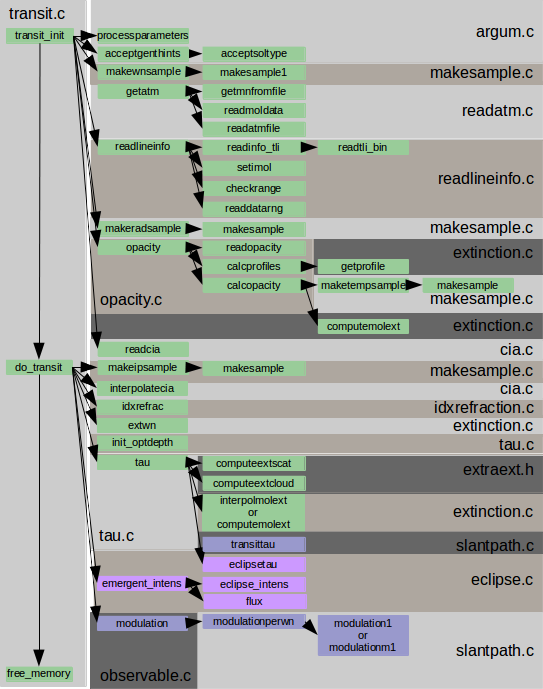
\includegraphics{fig/transit_diagram}
\label{fig:codediagram}
\caption{{\tt transit} function structure. The boxes contain function names, and arrows point from a function to the function it calls. Functions are called from left to right, then top to bottom. For example, at the beginning, transit\_init calls processparameters, then transit\_init calls acceptgenhints, then acceptgenhints calls acceptsoltype, and so on. Boxes are color-coded as follows:  purple functions are used for eclipse geometry, blue functions are used for transit geomtry, and green functions are used in both. The shaded backgrounds indicate where each function can be found.}
\end{figure}

In Section \ref{sec:headers} we describe all the headers included in {\tt transit}. Section \ref{sec:variables} gives all the custom variable types and their purpose. Then in Section \ref{sec:constants} we list all the defined constants in {\tt transit}. Section \ref{structures} lists both the structures and structure types used, and makes note of which function alters each array. In Section \ref{sec:functions} we list all source files and functions, and provide a list of the variables which are altered by each function along with a walkthrough of each major function. Finally, Section \ref{sec:equations} lists some equations that are important to the calculations made in {\tt transit}.
\pagebreak
\section{List of Headers used by \texttt{transit}}
This section lists all headers included in the {\tt transit} program. Those which are unique to {\tt transit} can be found in the transit/include/ directory. The file transit.h contains the lines which include the rest of the headers.
\label{sec:headers}
\begin{table}[ht]
\centering
\caption{Headers}
\label{table:headers}
\begin{tabular}{ll}
\hline
\hline
Name            & Description \\
\hline
transit.h       &  Radius and wavelength indices \\
stdarg.h        &  Record indices \\
math.h          &  Partition-function data \\
errno.h         &  Line-transition data  \\
sys/types.h     &  Partial result  \\
sys/stat.h      &  Atmospheric data  \\
sts/time.h      &  Cross-section data  \\
unistd.h        &  Collision-induced absorption data  \\
sampling.h      &  Voigt profile data type \\
profile.h       &  Precise Voigt profile data type \\
iomisc.h        &  Declares miscellaneous input/output functions \\
xmalloc.h       &  Redefines \ttblue{malloc, realloc, calloc} \\
strings.h       &  Defines several string manipulation functions \\
stdlib.h        &  Defines many general purpose functions \\
stdio.h         &  Defines many general input/output functions \\
alloca.h        &  Defines \ttblue{alloca}, which allocates temporary memory \\
flags\_tr.h     &  Defines {\tt transit} flags \\
constants\_tr.h &  Defines {\tt transit} constants (see Table \ref{table:constants}) \\
types\_tr.h     &  Defines {\tt transit} custom variable types (see Table \ref{table:types}) \\
\hline
\end{tabular}
\end{table}

\pagebreak	
\section{List of Custom Variable Types in \texttt{transit} DONE}
\label{sec:variables}
Table \ref{table:types} lists the user-defined data types used in
Transit.  These declarations are located in
transit/transit/include/types\_tr.h.

\begin{table}[ht]
\centering
\caption{Custom Variable Types}
\label{table:types}
\begin{tabular}{lll}
\hline
\hline
Name         & Type   & Description \\
\hline
PREC\_NSAMP  & int    &  Radius and wavelength indices \\
PREC\_NREC   & long   &  Record indices \\
PREC\_ZREC   & double &  Partition-function data \\
PREC\_LNDATA & double &  Line-transition data  \\
PREC\_RES    & double &  Partial result  \\
PREC\_ATM    & double &  Atmospheric data  \\
PREC\_CS     & double &  Cross-section data  \\
PREC\_VOIGT  & float  &  Voigt profile data type \\
PREC\_VOIGTP & double &  Precise Voigt profile data type \\
\hline
\end{tabular}
\end{table}
\pagebreak

\section{List of Constants in \texttt{transit} DONE}
\label{sec:constants}
Table \ref{table:constants} lists the user-defined constants used in \texttt{transit}. The definitions can be found in transit/transit/include/constants\_tr.h.
\begin{table}[ht]
\centering
\caption{Constants}
\label{table:constants}
\begin{tabular}{lll}
\hline
\hline
Name         & Value                                       & Description \\
\hline
RHOSTP       & 1.29e-3 g cm\sp{-3}                         &  Density at STP \\
PI           & 3.141592653589793                           &  Pi \\
DEGREES      & PI/180.0                                    &  Radians per degree \\
GGRAV        & 6.673e-8 erg cm g\sp{2}                     &  Gravitational constant  \\
HOUR         & 3600.0 s                                    &  Seconds per hour   \\
AU           & 14959786896040.492 cm                       &  Centimeters per AU  \\
ANGSTROM     & 1e-8 cm                                     &  Centimeters per angstrom  \\
SUNMASS      & 1.9891e33 g                                 &  Mass of the sun  \\
SUNRADIUS    & 6.95508e10 cm                               &  Radius of the sun \\
AMU          & 1.66053886e-24 g                            &  Grams per atomic mass unit \\
LO           & 2.686763e19 cm\sp{-3}                       &  Loschmidt constant \\
EC           & 4.8032068e-10 statC                         &  Electron charge \\
LS           & 2.99792458e10 cm s\sp{-1}                   &  Light speed \\
ME           & 9.1093897e-28 g                             &  Mass of an electron \\
KB           & 1.380658e-16 erg K\sp{-1}                   &  Boltzmann constant \\
H            & 6.6260755e-27 erg s                         &  Planck constant \\
HC           & H*LS erg cm                                 &  Planck constant $\times$ speed of light \\
SIGCTE       & (PI*EC\sp{2})/(LS\sp{2}*ME*AMU) cm g\sp{-1} &  Cross-section constant \\
EXPCTE       & (H*LS)/KB cm K                              &  Exponent constant \\
ONEOSQRT2PI  & 0.3989422804                                &  1/sqrt(2pi) \\
SQRTLN2      & 0.83255461115769775635                      &  sqrt(ln(2)) \\
MAXNAMELEN   & 20                                          &  Maximum length of name strings \\
\hline
\end{tabular}
\end{table}
\pagebreak
\section{List of Structures in the \texttt{transit} Files}
\label{structures}
\subsection{Structure Types}

Sampling properties of impact parameter, wavenumber, etc.
\begin{plain}                            
typedef struct {    
  PREC_NREC n;      /* Number of elements                                   */
  PREC_RES d;       /* Spacing                                              */
  PREC_RES i;       /* Initial value                                        */
  PREC_RES f;       /* Final value                                          */
  int o;            /* Oversampling                                         */
  PREC_RES *v;      /* Values of the sampling                               */
    /* ALLOCATED:	getatm						    */
    /* ALLOCATED:	readatmfile					    */
    /* FILLED OUT:	readatmfile					    */
    /* FILLED OUT:	radpress					    */
    /* FREED: 		freemem_samp					    */
  double fct;       /* v units factor to cgs                                */
} prop_samp;
\end{plain}

\noindent \newline
Isotopes' variable information.
\begin{plain}
typedef struct {    
  unsigned int n;   /* Arrays' length                                       */
  double *z;        /* Partition function [radius or temp]                  */
    /* ALLOCATED:	readtli_bin					    */
    /* FILLED OUT:	readtli_bin					    */
    /* FREED: 		free_isov						    */ 
} prop_isov;
\end{plain}
\noindent \newline
Isotopes' fixed information.
\begin{plain}
typedef struct {    
  int d;            /*  Database to which they belong */
  char *n;          /*  Isotope name                  */
  PREC_ZREC m;      /*  Isotope mass                  */
} prop_isof;
\end{plain}
\noindent \newline
Molecule properties.
\begin{plain}
typedef struct{   
  int n;           /*  Number of elements      */
  PREC_ATM *d;     /*  Density   [n]           */
    /* ALLOCATED:	getatm						    */
    /* ALLOCATED:	readatmfile					    */
    /* FILLED OUT:	makeradsample					    */
    /* FREED: 		free_mol					    */ 
  PREC_ATM *q;     /*  Abundance [n]           */
    /* ALLOCATED:	getatm						    */
    /* ALLOCATED:	readatmfile					    */
    /* FILLED OUT:	makeradsample					    */
    /* FREED: 		free\_mol					    */ 
} prop_mol;
\end{plain}
\noindent \newline
Atmosphere properties.
\begin{plain}
typedef struct {    
  double *mm;       /*  Mean molecular mass [rad]        */
    /* ALLOCATED:	getatm						    */
    /* ALLOCATED:	readatmfile					    */
    /* FILLED OUT:	makeradsample					    */
    /* FREED: 		free_atm					    */ 
  PREC_ATM *p;      /*  Pressure    [rad]                */
    /* ALLOCATED:	getatm						    */
    /* ALLOCATED:	readatmfile					    */
    /* FILLED OUT:	makeradsample					    */
    /* FREED: 		free_atm					    */ 
  PREC_ATM *t;      /*  Temperature [rad]                */
    /* ALLOCATED:	getatm						    */
    /* ALLOCATED:	readatmfile					    */
    /* FILLED OUT:	makeradsample					    */
    /* FREED: 		free_atm					    */ 
  PREC_ATM pfct;    /*  p units factor to cgs (dyne/cm2) */
  PREC_ATM tfct;    /*  t units factor to cgs (Kelvin)   */
} prop_atm;
\end{plain}
\noindent \newline
Database properties.
\begin{plain}
typedef struct {    
  char *n;          /*  Database name                                        */
  char *molname;    /*  Molecule name                                        */
  unsigned int i;   /*  Number of isotopes                                   */
  int s;            /*  Cumulative first isotope's index                     */
} prop_db;
\end{plain}

\noindent \newline
Database temperatures.
\begin{plain}
typedef struct {    
  unsigned int t;   /* Number of temperatures				    */
  double *T;        /* Temperatures                                         */
    /* ALLOCATED:	readtli_bin					    */
    /* FILLED OUT:	readtli_bin					    */
    /* FREED: 		free_dbnoext					    */
} prop_dbnoext;
\end{plain}

\noindent \newline
Ray solution parameters and integrator functions.
\begin{plain}
typedef struct {
  const char *name;          /* Ray solution name                           */
  const char *file;          /* Ray solution source file                    */
  const short monospace;     /* Request equispaced inpact parameter?        */
  PREC_RES (*optdepth)       /* Extinction-coefficient integrator function  */
       (struct transit *tr,
        PREC_RES b,              /* Height of ray path                      */
        PREC_RES *ex);           /* Extinction array [rad]                  */
  PREC_RES (*spectrum)       /* Optical-depth integrator function           */
        (struct transit *tr,
         PREC_RES *tau,          /* Optical depth                           */
         PREC_RES w,             /* Wavenumber value                        */
         long last,              /* index where tau exceeded toomuch        */
         PREC_RES toomuch,       /* Cutoff optical depth                    */
         prop_samp *r);          /* Impact parameter or layers' radius      */
} ray_solution;	transit.h:
\end{plain}


\subsection{Structures}

Proportional-abundance isotopic parameters.
\begin{plain}
struct atm_isoprop{
  double f;            /* Fractional abundance                        */
  double m;            /* Isotope mass                                */
  int eq;              /* Isotope index from transit.ds.isotopes      */
  char n[maxeisoname]; /* Isotope name                                */
  char t[maxeisoname]; /* Molecule name                               */
};
\end{plain}

\noindent \newline
Line transition parameters
\begin{plain}
struct line_transition{
  PREC_LNDATA *wl;       /* Wavelength                                      */
    /* ALLOCATED:	readdatarng					    */
    /* FILLED OUT:	readdatarng					    */
    /* FREED: 		freemem_linetranstion				    */ 
  PREC_LNDATA *elow;     /* Lower-state energy                              */
    /* ALLOCATED:	readdatarng					    */
    /* FILLED OUT:	readdatarng					    */
    /* FREED: 		freemem_linetranstion				    */ 
  PREC_LNDATA *gf;       /* gf value                                        */
    /* ALLOCATED:	readdatarng					    */
    /* FILLED OUT:	readdatarng					    */
    /* FREED: 		freemem_linetransition				    */ 
  short *isoid;          /* Isotope ID (Assumed to be in range)             */
    /* ALLOCATED:	readdatarng					    */
    /* FILLED OUT:	readdatarng					    */
    /* FREED: 		freemem_linetransition				    */ 
  double wfct;           /* wl units factor to cgs                          */
  double efct;           /* elow units factor to cgs                        */
};
\end{plain}

\noindent \newline
Line information parameters
\begin{plain}
struct lineinfo{
  struct line_transition lt; /* Line transitions                            */
  unsigned short tli_ver;    /* TLI version                                 */
  unsigned short lr_ver;     /* lineread version                            */
  unsigned short lr_rev;     /* lineread revision                           */
  double wi, wf;             /* Initial and final wavelength in database    */
  long endinfo;              /* Position at the end of the info part
                                of the info file                            */
  int ni;                    /* Number of isotopes                          */
  int ndb;                   /* Number of databases                         */
  prop_isov *isov;           /* Variable isotope information (w/temp) [iso] */
    /* ALLOCATED:	readtli_bin					    */
    /* FILLED OUT:	readtli_bin					    */
    /* FREED: 		freemem_lineinfo				    */ 
  prop_dbnoext *db;          /* Temperature info from databases [DB]        */
    /* ALLOCATED:	readtli_bin					    */
    /* FILLED OUT:	readtli_bin					    */
    /* FREED: 		freemem_lineinfo				    */ 
  PREC_NREC n_l;             /* Number of lines in database                 */
};
\end{plain}

\noindent \newline
Atmospheric data file parameters.
\begin{plain}
struct atm_data{
  int n_aiso;            /* Number of molecules in atmosphere file          */
  prop_samp rads;        /* Radius sampling                                 */
  prop_atm atm;          /* Atmospheric properties                          */
  prop_mol *molec;       /* Molecular information [n_aiso]                  */
    /* ALLOCATED:	getatm						    */
    /* FILLED OUT:	getmoldata, getmnfromfile			    */
    /* FREED: 		free_mol					    */ 
  double *mm;            /* Mean molecular mass [rad]                       */
    /* ALLOCATED:	getatm						    */
    /* ALLOCATED:       readatmfile                                         */
    /* FILLED OUT:	getmoldata					    */
    /* FREED: 		freemem_atmosphere				    */ 
  char *info;            /* Optional atmosphere file information or label   */
  _Bool mass;            /* Abundances in isov by mass (1) of by number (0) */
  int begline;           /* Line of first radius dependent info             */
  long begpos;           /* Position of first radius dependent info         */
};
\end{plain}

\noindent \newline
Extinction array and extinction parameters.
\begin{plain}
struct extinction{
  PREC_RES **e;      /* Extinction value [rad][wav]                         */
    /* ALLOCATED:	extwn						    */
    /* FILLED OUT:      computemolext, interpolmolext			    */
    /* FREED: 		freemem_extinction				    */ 
  int vf;            /* Number of fine-bins of the Voigt function           */
  float ta;          /* Number of alphas that have to be contained in
                        the profile                                         */
  _Bool *computed;   /* Whether the extinction at the given radius was
                        computed [rad]                                      */
    /* ALLOCATED:	extwn						    */
    /* FILLED OUT:      computemolext, interpolmolext			    */
    /* FREED: 		freemem_extinction				    */
  double ethresh;    /* Lower extinction-coefficient threshold              */
};
\end{plain}

\noindent \newline
Opacity array and opacity parameters.
\begin{plain}
struct opacity{
  PREC_RES ****o;         /* Opacity grid [temp][iso][rad][wav]             */
    /* ALLOCATED:	calcopacity, readopacity			    */
    /* FILLED OUT:      computemolext					    */
    /* FREED: 		freemem_opacity					    */ 
  PREC_VOIGT ***profile;  /* Voigt profiles [nDop][nLor][2*profsize+1]      */
    /* ALLOCATED:	calcprofiles, getprofile			    */
    /* FILLED OUT:	getprofile					    */
    /* FREED: 		freemem_opacity					    */ 
  PREC_NREC **profsize;   /* Half-size of Voigt profiles [nDop][nLor]       */
    /* ALLOCATED:	calcprofiles					    */
    /* FILLED OUT:	getprofile					    */
    /* FREED: 		freemem_opacity					    */ 
  double *aDop,           /* Sample of Doppler widths [nDop]                */
    /* ALLOCATED:	calcprofiles					    */
    /* FILLED OUT:	calcopacity					    */
    /* FREED: 		freemem_opacity					    */ 
         *aLor;           /* Sample of Lorentz widths [nLor]                */
    /* ALLOCATED:	calcprofiles					    */
    /* FILLED OUT:	calcopacity					    */
    /* FREED: 		freemem_opacity					    */ 
  PREC_RES *temp,         /* Opacity-grid temperature array                 */
    /* ALLOCATED:	calcopacity					    */
    /* FILLED OUT:	calcopacity					    */
    /* FREED: 		freemem_opacity					    */ 
           *press,        /* Opacity-grid pressure array                    */
    /* ALLOCATED:	calcopacity					    */
    /* FILLED OUT:	calcopacity					    */
    /* FREED: 		freemem_opacity					    */ 
           *wns;          /* Opacity-grid wavenumber array                  */
    /* ALLOCATED:	calcopacity					    */
    /* FILLED OUT:	calcopacity					    */
    /* FREED: 		freemem_opacity					    */ 
  PREC_ATM **ziso;        /* Partition function per isotope [niso][Ntemp]   */
    /* ALLOCATED:	calcopacity					    */
    /* FILLED OUT:	calcopacity					    */
    /* FREED: 		freemem_opacity					    */ 
  int *molID;             /* Opacity-grid molecule ID array                 */
    /* ALLOCATED:	calcopacity					    */
    /* FILLED OUT:	calcopacity					    */
    /* FREED: 		freemem_opacity					    */ 
  long Nwave, Ntemp, Nlayer, Nmol, /* Number of elements in opacity grid    */
      nDop, nLor;         /* Number of Doppler and Lorentz-width samples    */
};
\end{plain}

\noindent \newline
Index of refraction array.
\begin{plain}
struct idxref{
  PREC_RES *n;   /* Index of refraction [rad]                               */
    /* ALLOCATED:	idxrefrac					    */
    /* FILLED OUT:	idxrefrac					    */
    /* FREED: 		freemem_idxrefrac				    */ 
};
\end{plain}

\noindent \newline
Save file information.
\begin{plain}
#if 0
struct savefiles {
  char *ext;         /* saves extinction            */
  char *tau;  	     /* after tau() savefile        */
  char *modulation;  /* after modulation() savefile */
};
#endif
\end{plain}

\noindent \newline
Optical depth array and related information.
\begin{plain}
struct optdepth{
  PREC_RES **t;     /* Optical depth [wn][ip]                               */
    /* ALLOCATED:       init_optdepth					    */
    /* FILLED OUT:      tau						    */
    /* FREED:           freemem_tau					    */
  long *last;       /*  Level index where the optical depth reached toomuch
                       (counting from the top of the atmosphere) [wn]       */
    /* ALLOCATED:       init_optdepth                                       */
    /* FILLED OUT:      tau						    */
    /* FREED:           freemem_tau					    */
  double toomuch;   /* Optical depth values greater than this won't be
                       calculated: the extinction is assumed to be zero.    */
};
\end{plain}

\noindent
Intensity array.
\begin{plain}
struct grid{
  PREC_RES **a;      /* Intensity grid, 2D, [an][wnn]                       */
    /* ALLOCATED:	init_optdepth					    */
    /* FILLED OUT:	eclipse_intens					    */
    /* FREED: 		freemem_intensityGrid				    */ 
};
\end{plain}

\noindent
Information about the geometry of the transit or eclipse.
\begin{plain}
struct geometry{
  float smaxis;       /* Semimajor axis                                     */
  double smaxisfct;   /* 'smaxis' times this gives cgs units.               */
  double time;        /* this value is 0 when in the middle of the eclipse  */
  double timefct;     /* 'time' times this gives cgs units                  */
  float incl;         /* inclination of the planetary orbit with respect
                         to the observer, 90 degrees is edge on             */
  float inclfct;      /* Units to convert inclination to radians            */
  double ecc;         /* eccentricty                                        */
  double eccfct;      /* eccentricity's units                               */
  double lnode;       /* longitude of the ascending node                    */
  double lnodefct;    /* longitude of the ascending node units              */
  double aper;        /* argument of the pericenter                         */
  double aperfct;     /* argument of the pericenter units                   */

  double starmass;    /* Mass of the star                                   */
  double starmassfct; /* 'starmass' times this gives cgs units.             */

  double starrad;     /* Star's radius                                      */
  double starradfct;  /* 'starrad' times this gives cgs units.              */

  double x, y;        /*  Coordinates of the center of the planet with
                         respect to the star. 'fct' to convert to cgs is
                         found in rads.fct. These fields are not hinted.    */

  _Bool transpplanet; /* If true, set maximum optical depth to toomuch      */
};
\end{plain}

\noindent
Isotope information.
\begin{plain}
struct isotopes{
  prop_isof *isof;    /* Fixed isotope information      [n_i]               */
    /* ALLOCATED:	readtli_bin					    */
    /* FILLED OUT:	readtli_bin					    */
    /* FREED: 		freemem_isotopes				    */ 
  prop_isov *isov;    /* Variable isotope information   [n_i]               */
    /* ALLOCATED:	readtli_bin			                    */
    /* FILLED OUT:	readdatarng					    */
    /* FREED: 		freemem_isotopes				    */ 
  double *isoratio;   /* Isotopic abundance ratio       [n_i]               */
    /* ALLOCATED:	readtli_bin      				    */
    /* FILLED OUT:	readtli_bin					    */
    /* FREED: 		freemem_isotopes				    */ 
  int *imol;          /* Molecule index for this isotope[n_i]               */
    /* ALLOCATED:	readlineinfo					    */
    /* FILLED OUT:	setimol						    */
    /* FREED: 		freemem_isotopes				    */ 
  prop_db *db;        /* Database's info [n_db]                             */
    /* ALLOCATED:	readtli_bin					    */
    /* FILLED OUT:	readtli_bin					    */
    /* FREED: 		freemem_isotopes				    */ 
  int n_db,           /* Number of databases                                */
      n_i,            /* Number of isotopes                                 */
      nmol;           /* Number of different molecules having a line list   */
};
\end{plain}

\noindent
Molecule information.
\begin{plain}
struct molecules{
  int nmol;           /* Number of molecules                                */
  prop_mol *molec;    /* Molecular properties                               */
    /* ALLOCATED:	getatm						    */
    /* FILLED OUT:	makeradsample					    */
    /* FREED: 		free_mol					    */ 
  char **name;        /* Molecules' names                                   */
    /* ALLOCATED:	getmnfromfile					    */
    /* FILLED OUT:	getmnfromfile					    */
    /* FREED: 		freemem_molecules				    */ 
  PREC_ZREC *mass;    /* Molecules' masses                                  */
    /* ALLOCATED:	getatm						    */
    /* FILLED OUT:	getmoldata					    */
    /* FREED: 		freemem_molecules				    */ 
  PREC_ZREC *radius;  /* Molecules' radii                                   */
    /* ALLOCATED:	getatm						    */
    /* FILLED OUT:	getmoldata					    */
    /* FREED: 		freemem_molecules				    */ 
  int *ID;            /* Molecule universal ID                              */
    /* ALLOCATED:	getatm						    */
    /* FILLED OUT:	getmoldata					    */
    /* FREED: 		FINDME: this isn't freed!			    */ 
};
\end{plain}

\noindent
Flux
\begin{plain}
struct outputray{
  PREC_RES *o;     /* Output as seen before interaction with telescope      */
    /* ALLOCATED:	flux, modulation				    */
    /* FILLED OUT:	flux, modulation1, moldulationm1		    */
    /* FREED: 		freemem_outputray				    */ 
};
\end{plain}

\noindent
Cloud extinction information.
\begin{plain}
struct extcloud{
  double cloudext;     /* Maximum opacity in [cm-1]                          */
  double cloudtop;     /* Radius at which clouds start                       */
  double cloudbot;     /* Radius at which clouds has it maximum thickness
                          'cloudext'.                                        */
};
\end{plain}

\noindent
Scattering extinction information.
\begin{plain}
struct extscat{
  double prm;
};
\end{plain}

\noindent
Saved extinction grid name.
\begin{plain}
struct saves{
  char *ext;   /* Extinction grid                                           */
};
\end{plain}

\noindent
Stores requested extinction, optical depth, or CIA detailed information.
\begin{plain}
struct detailfld{
  int n;         /* Number of requested wavenumber samples */
  PREC_RES *ref; /* Array of wavenumbers requested         */
    /* ALLOCATED:	processparameters				    */
    /* FILLED OUT:	acceptgenhints					    */
    /* FREED: 		freemem_detailfld				    */ 
  char file[80]; /* Output filename                        */
  char name[30]; /* Name of field                          */
};
\end{plain}

\noindent
Detailed output for extinction, optical depth, or CIA.
\begin{plain}
struct detailout{
  struct detailfld ext, tau, cia;
};
\end{plain}

\noindent
Cross-section extinction information.
\begin{plain}
struct cross{
  int nfiles;       /* Number of CS files                                  */
  PREC_CS **e;     /* Extinction from all CS sources [wn][temp]           */
    /* ALLOCATED:	readcs						    */
    /* FILLED OUT:      interpolatecs					    */
    /* FREED:           freemem_cs					    */ 
  PREC_CS ***cs;  /* Tabulated CS extinction      [nfiles][nwave][ntemp] */
    /* ALLOCATED:	readcs						    */
    /* FILLED OUT:	readcs						    */
    /* FREED:           freemem_cs					    */ 
  PREC_CS **wn;    /* Tabulated wavenumber  arrays  [nfiles][nwave]        */
    /* ALLOCATED:	readcs						    */
    /* FILLED OUT:	readcs						    */
    /* FREED:           freemem_cs					    */ 
  PREC_CS **temp;  /* Tabulated temperature arrays  [nfiles][ntemp]        */
    /* ALLOCATED:	readcs						    */
    /* FILLED OUT:	readcs						    */
    /* FREED:           freemem_cs					    */ 
  int *nwave;       /* Number of wavenumber samples  [nfiles]               */
    /* ALLOCATED:	readcs						    */
    /* FILLED OUT:	readcs						    */
    /* FREED:           freemem_cs					    */ 
  int *ntemp;       /* Number of temperature samples [nfiles]               */
    /* ALLOCATED:	readcs						    */
    /* FILLED OUT:	readcs						    */
    /* FREED:           freemem_cs					    */ 
  int *mol1, *mol2; /* Pairs of molecule's ID        [nfiles]               */
    /* ALLOCATED:	readcs						    */
    /* FILLED OUT:	readcs						    */
    /* FREED:           freemem_cs					    */ 
};
\end{plain}

\noindent
Structure containing all user-given information that is passed to the transit structure upon approval.
\begin{plain}                                                 */
struct transithint{  
  char *f_atm,          /* Atmosphere filename                              */
       *f_line,         /* TLI filename                                     */
       *f_opa,          /* Opacity filename                                 */
       *f_out,          /* Output (main) filename                           */
       *f_toomuch,      /* Output toomuch filename                          */
       *f_outsample,    /* Output sample filename                           */
       *f_molfile;      /* Known molecular info filename                    */
  PREC_NREC ot;         /* Radius index at which to print output from tau   */
  prop_samp rads, ips,  /* Sampling properties of radius, impact parameter, */
       wavs, wns, temp;   /* wavelength, wavenumber, and temperature        */
  char *angles;         /* String with incident angles (for eclipse)        */
  char *qmol, *qscale;  /* String with species scale factors                */
  float allowrq;        /* How much less than one is accepted, and no warning
                           is issued if abundances don't ad up to that      */
  float timesalpha;     /* Number of alphas that have to be contained in a
                           calculated profile, one side only                */
  int voigtfine;        /* Fine-binning for Voigt function in kapwl(), if
                           accepted it goes to tr.ds.op.vf                   */
  int nDop, nLor;       /* Number of broadening width samples                */
  float dmin, dmax, lmin, lmax; /* Broadening-width samples boundaries       */
  int verbnoise;        /* Noisiest verbose level in a non debugging run     */ 
  _Bool mass;           /* Whether the abundances read by getatm are by
                           mass or number                                    */
  _Bool opabreak;       /* Break after opacity calculation flag              */
  long fl;              /* flags                                             */
  _Bool userefraction;  /* Whether to use variable refraction                */
  double p0, r0;        /* Pressure and radius reference level               */
  double gsurf;         /* Surface gravity                                   */

  double toomuch;       /* Optical depth values greater than this won't be
                           calculated: the extinction is assumed to be zero  */
  int taulevel;         /* Tau integration level of precision                */
  int modlevel;         /* Modulation integration level of precision         */
  char *solname;        /* Name of the type of solution                      */
  struct geometry sg;   /* System geometry                                   */
  struct saves save;    /* Saves indicator of program stats                  */

  struct extcloud cl;
  struct detailout det;

  double ethresh;       /* Lower extinction-coefficient threshold            */
  char **csfile;
  int ncross;
};
\end{plain}

\noindent
Main data structure. 
\begin{plain}
struct transit{  
  char *f_atm,       /* Atmosphere filename                                 */
       *f_line,      /* TLI filename                                        */
       *f_opa,       /* Opacity filename                                    */
       *f_out,       /* Output (main) filename                              */
       *f_toomuch,   /* Output toomuch filename                             */
       *f_outsample, /* Output sample filename                              */
       *f_molfile;   /* Known molecular info filename                       */
  PREC_NREC ot;      /* Radius index at which to print output from tau      */

  FILE *fp_atm, *fp_opa, *fp_out, *fp_line; /* Pointers to files            */
  float allowrq;    /* How much less than one is accepted, so that no warning
                       is issued if abundances don't ad up to that          */
  PREC_RES telres;  /* Telescope resolution                                 */
  long int angleIndex; /* Index of the current angle                        */
  prop_samp rads,      /* Sampling properties of radius,                    */
    /* ALLOCATED:	makesample, makesample1				    */
    /* FILLED OUT:	makeradsample					    */
    /* FREED: 		freemem_samp					    */
            ips,       /* impact parameter,                                 */
    /* ALLOCATED:	makesample, makesample1				    */
    /* FILLED OUT:	makeipsample					    */
    /* FREED: 		freemem_samp					    */
            owns,      /* oversampled wavenumber,                           */
    /* ALLOCATED:	makesample, makesample1				    */
    /* FILLED OUT:	makewnsample					    */
    /* FREED: 		freemem_samp					    */
            wavs,      /* wavelength,                                       */
    /* ALLOCATED:	makesample, makesample1				    */
    /* FILLED OUT:	FINDME						    */
    /* FREED: 		freemem_samp					    */
            wns,       /* wavenumber,                                       */
    /* ALLOCATED:	makesample, makesample1				    */
    /* FILLED OUT:	makewnsample					    */
    /* FREED: 		freemem_samp					    */
            temps;     /* temperature                                       */
    /* ALLOCATED:	makesample, makesample1				    */
    /* FILLED OUT:	maketempsample					    */
    /* FREED: 		freemem_samp					    */
  prop_atm atm;      /* Sampled atmospheric data                            */
  _Bool opabreak;    /* Break after opacity calculation                     */
  int ndivs,         /* Number of exact divisors of the oversampling factor */
     *odivs;         /* Exact divisors of the oversampling factor           */
    /* ALLOCATED:	makewnsample					    */
    /* FILLED OUT:	makewnsample					    */
    /* FREED: 		FINDME: not freed?				    */ 
  int voigtfine;     /* Number of fine-bins of the Voigt function           */
  float timesalpha;  /* Broadening profile width in number of Doppler or
                        Lorentz half width                                  */
  double p0, r0;     /* Pressure and radius reference level                 */
  double gsurf;      /* Surface gravity                                     */
  int ann;           /* Number of angles                                    */
  double *angles;    /* Array of incident angles for eclipse geometry       */
    /* ALLOCATED:	acceptgenhints					    */
    /* FILLED OUT:	acceptgenhints					    */
    /* FREED: 		FINDME						    */ 
  int nqmol;         /* Number of species scale factors                     */
  double *qscale;    /* Species scale factors                               */
    /* ALLOCATED:	acceptgenhints					    */
    /* FILLED OUT:	acceptgenhints					    */
    /* FREED: 		FINDME						    */ 
  int *qmol;         /* Species with scale factors                          */
    /* ALLOCATED:	acceptgenhints					    */
    /* FILLED OUT:	acceptgenhints					    */
    /* FREED: 		FINDME						    */ 
  int taulevel;      /* Tau integration level of precision                  */
  int modlevel;      /* Modulation integration level of precision           */

  long fl;           /* flags                                               */
  long interpflag;   /* Interpolation flag                                  */
  long pi;           /* progress indicator                                  */

  ray_solution *sol; /* Transit solution type                               */
  PREC_RES *outpret; /* Output dependent on wavelength only as it travels
                        to Earth before telescope                           */
    /* ALLOCATED:	FINDME						    */
    /* FILLED OUT:	FINDME						    */
    /* FREED: 		freemem_transit					    */ 

  struct saves save; /* Saves indicator of program stats                    */

  struct {           /* Data structures pointers, this is data that is not
                        required for the final computation                  */
    struct transithint *th;
    struct lineinfo    *li;
    struct atm_data    *at;
    struct extinction  *ex;
    struct opacity     *op;
    struct grid        *intens;
    struct optdepth    *tau;
    struct idxref      *ir;
    struct geometry    *sg;
#if 0
    struct savefiles   *sf;
#endif
    struct isotopes    *iso;
    struct molecules   *mol;
    struct outputray   *out;
    struct extcloud    *cl;
    struct extscat     *sc;
    struct detailout   *det;
    struct cross       *cross;
  }ds;
};
\end{plain}

\newpage
\section{List of Functions in the \texttt{transit} Files}
\label{sec:functions}
In this section we list all functions, sorted by source file, give a brief description of what they do, list all variables that they alter, and provide a walkthrough for each. A modified variable is written in \ttred{red}, a function is written in \ttblue{blue}, and an unmodified variable is written in {\tt typewriter}. Unless impractical, each subsection has a diagram which indicates the function structure of that source file.

\subsection{transit.c}
This file contains the main {\tt transit} driver functions. The \ttblue{main} function calls \ttblue{transit\_init} and \ttblue{do\_transit}, the driver functions which do the initialization and calculation. Then \ttblue{main} calls \ttblue{free\_memory} which frees the remaining memory. This structure is shown in Figure \ref{fig:transitc}.

\begin{figure}
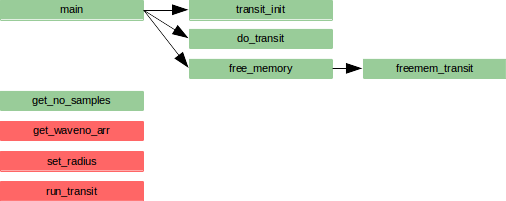
\includegraphics{fig/transitc}
\caption{Function structure of transit.c. The boxes contain function names, and arrows point from a function to the function it calls. Functions are called from left to right, then top to bottom. Boxes are color-coded as follows:  purple functions are used for eclipse geometry, blue functions are used for transit geometry, green functions are used in both, and red functions are unused at this time.}
\label{fig:transitc}
\end{figure}

\subsubsection{List of Functions Defined in transit.c}
\function{
void transit\_init(int argc, char **argv)}
\tgray{This function initializes the structures used in \tt{transit}.} \newline

\function{
int get\_no\_samples(void)}
\tgray{Returns the size of the wavenumber sampling array.} \newline

\function{
void get\_waveno\_arr(double *waveno\_arr, int waveno)}
\tgray{Fills the given array with the wavenumber sampling values.} \newline

\function{
void set\_radius(double refradius)}
\tgray{Set the reference radius in the transit structure}.\newline

\function{
void run\_transit(double *re\_input, int transitint, double *transit\_out, \\ int transit\_out\_size)}
\tgray{Driver function that loads the atmospheric file and runs transit.} \newline

\function{
void do\_transit(double *transit\_out)}
\tgray{Driver function that calls all the functions to do calculations and then free the created arrays.} \newline

\function{
void free\_memory(void)}
\tgray{Driver function that calls functions which free the rest of memory using in {\tt transit}.} \newline

\function{
int main(int argc, char **argv)}
\tgray{Main driver function which calls functions to initialize, run, and then free {\tt transit}.} \newline

\function{
void freemem\_transit(struct transit *tr)} 
\tgray{Free the transit structure} \newline

\subsubsection{transit\_init}
\paragraph{Walkthrough}
\begin{enumerate}[leftmargin=10pt, noitemsep, parsep=0pt, topsep=0ex]
\item[-] Initialize the transit structure to 0.
\item[-] Call \ttblue{processparameters} from argum.c to process the command line arguments and store them in the hint structure.
\item[-] Call \ttblue{acceptgenhints} from argum.c to accept general hints from the hint structure.
\item[-] Call \ttblue{printintro} from argum.c to print the introductory message.
\item[-] Call \ttblue{makewnsample} from makesample.c to create the wavenumber sampling.
\item[-] Call \ttblue{getatm} from readatm.c to read the atmospheric file.
\item[-] Call \ttblue{readlineinfo} from readlineinfo.c to read the TLI file.
\item[-] Call \ttblue{makeradsample} from makesample.c to create the radius sampling.
\item[-] Call \ttblue{opacity} from opacity.c to calculate the opacity grid.
\item[-] Call \ttblue{readcs} from crosssec.c to read CS file(s).
\item[-] Set boolean to indicate that {\tt transit} has been initiated.
\end{enumerate}

\subsubsection{get\_no\_samples}
\paragraph{Walkthough}
\begin{enumerate}[leftmargin=10pt, noitemsep, parsep=0pt, topsep=0ex]
\item[-] Return the size of the wavenumber array
\end{enumerate}

\subsubsection{get\_waveno\_arr}
\paragraph{Walkthrough}
\begin{enumerate}[leftmargin=10pt, noitemsep, parsep=0pt, topsep=0ex]
\item[-] If \ttblue{transit\_init} has been run, fill out the given array with the wavenumber sampling values.
\item[-] Otherwise, indicate that \ttblue{transit\_init} has not been run and fill the given array with -1.
\end{enumerate}

\subsubsection{set\_radius}
\paragraph{Variables Modified}
\begin{enumerate}[leftmargin=10pt, noitemsep, parsep=0pt, topsep=0ex]
\item[-] Set \ttred{tr.r0} to the reference radius.
\end{enumerate}

\paragraph{Walkthrough}
\begin{enumerate}[leftmargin=10pt, noitemsep, parsep=0pt, topsep=0ex]
\item[-] Set the reference radius in the transit structure.
\end{enumerate}

\subsubsection{run\_transit}
\paragraph{Walkthrough}
\begin{enumerate}[leftmargin=10pt, noitemsep, parsep=0pt, topsep=0ex]
\item[-] Call \ttblue{realoadatm} from readatm.c to reload the atmospheric data.
\item[-] Call \ttblue{do\_transit} to run calculations.
\end{enumerate}
\subsubsection{do\_transit}
\paragraph{Variables Modified}
\begin{enumerate}[leftmargin=10pt, noitemsep, parsep=0pt, topsep=0ex]
\item[-] Fill in \ttred{tr.angleIndex}.
\item[-] Free \ttred{tr.save.ext}.
\end{enumerate}

\paragraph{Walkthrough}
\begin{enumerate}[leftmargin=10pt, noitemsep, parsep=0pt, topsep=0ex]
\item[-] If \ttblue{transit\_init} has been run:
\begin{enumerate}[leftmargin=10pt, noitemsep, parsep=0pt, topsep=0ex]
\item[-] Call \ttblue{makeipsample} from makesample.c to create the impact parameter sampling.
\item[-] Call \ttblue{interpcs} from crosssec.c to interpolate the cross-section grid.
\item[-] Call \ttblue{idxrefrac} from idxrefraction.c to compute the index of refraction.
\item[-] Call \ttblue{extwn} from extinction.c to calculate the extinction coefficient.
\item[-] Call \ttblue{init\_optdepth} to initialize optical depth structures.
\item[-] If using eclipse geometry:
\begin{enumerate}[leftmargin=10pt, noitemsep, parsep=0pt, topsep=0ex]
\item[-] Call \ttblue{tau} from tau.c to calculate optical depth as a function of radius.
\item[-] Loop over each angle.
\begin{enumerate}[leftmargin=10pt, noitemsep, parsep=0pt, topsep=0ex]
\item[-] Fill in angle indices.
\item[-] Call to \ttblue{emergent\_intens} from eclipse.c to calculate emergent intensity over the entire wavenumber range.
\end{enumerate}
\item[-] Call to \ttblue{flux} from eclipse.c to calculate the flux spectrum.
\item[-] Call to \ttblue{freemem\_intensityGrid} to free the intensity grid.
\end{enumerate}
\item[-] If using transit geometry:
\begin{enumerate}[leftmargin=10pt, noitemsep, parsep=0pt, topsep=0ex]
\item[-] Call to \ttblue{tau} to calculate optical depth as a fnction of radius.
\item[-] Call to \ttblue{modulation} to calculate transit modulation at each wavenumber.
\end{enumerate}
\item[-] Free the saved extinction grid.
\item[-] Call to \ttblue{freemem\_samp, freemem\_idexrefrac, freemem\_extinction, freemem\_tau, freemem\_outputray} to free the impact parameter sampling, index of refraction, extinction, optical depth, and output.
\item[-] Increment the number of iterations.
\end{enumerate}
\item[-] Otherwise warn that \ttblue{transit\_init} has not been run.
\end{enumerate}

\subsubsection{free\_memory}
\paragraph{Walkthrough}
\begin{enumerate}[leftmargin=10pt, noitemsep, parsep=0pt, topsep=0ex]
\item[-] Call to \ttblue{freemem\_molecules} to free molecular information.
\item[-] Call to \ttblue{freemem\_atmosphere} to free atmospheric data.
\item[-] If no opacity file was given (it was created), then call to \ttblue{freemem\_linetransition} to free the line transition data.
\item[-] Call to \ttblue{freemem\_lineinfo} to free line transition information.
\item[-] Call to \ttblue{freemem\_cs} to free cross-section data.
\item[-] Call to \ttblue{freemem\_transit} to free the transit structure.
\item[-] Reset transit initiation boolean to 0.
\end{enumerate}

\subsubsection{main}
\paragraph{Walkthrough}
\begin{enumerate}[leftmargin=10pt, noitemsep, parsep=0pt, topsep=0ex]
\item[-] Call to \ttblue{transit\_init} from transit.c to initialize the transit structures.
\item[-] Call to \ttblue{get\_no\_samples} from transit.c to get the number of wavenumber samples.
\item[-] Call to \ttblue{do\_transit} from transit.c to run the main calculations.
\item[-] Call to \ttblue{free\_memory} to free all remaining allocated memory.
\item[-] Return success.
\end{enumerate}

\subsection{transitstd.c:}
This file contains a number of standard functions. As they are largely unrelated, and called when necessary throughout the code, there is no relative structure to the functions in this file. Figure \ref{fig:transitstdc} shows the function structure of transitstd.c.

\begin{figure}
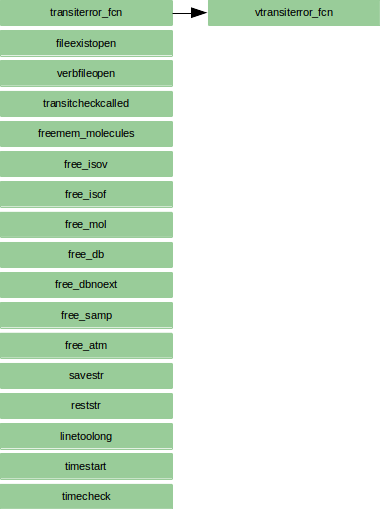
\includegraphics{fig/transitstdc}
\caption{Function structure of transitstd.c. The boxes contain function names, and arrows point from a function to the function it calls. Functions are called from left to right, then top to bottom.  Boxes are color-coded as follows:  purple functions are used for eclipse geometry, blue functions are used for transit geometry, green functions are used in both, and red functions are unused at this time.}
\label{fig:transitstdc}
\end{figure}

\subsubsection{List of Functions Defined in transitstd.c}
\function{
inline void transitdot(int thislevel, int verblevel, ...)}
\tgray{Print a '.' character.} \newline

\function{
int tr\_output\_fcn(int flags, const char *file, const long line, const char *str, ...)}
\tgray{Set up additional arguments and call the output function.} \newline

\function{
int tr\_output\_vfcn(int flags, const char *file, const long line, const char *str, \\ va\_list format)}
\tgray{Output, error, and debug function for {\tt transit}.} \newline

\function{
int fileexistopen(char *in, FILE **fp)}
\tgray{Check if a file exists and, if so, open it. Return various codes depending on what caused opening to fail.} \newline

\function{
FILE * verbfileopen(char *in, char *desc)}
\tgray{Handle various returns of \ttblue{fileexistopen}. Returns the file pointer or raises an error.} \newline

\function{
void transitcheckcalled(const long pi, const char *fcn, const int n, ...)}
\tgray{Check that the 'n' functions (given as variable argument) have been called before 'fnc'. Raise an error if they have not.} \newline

\function{
void error(int exitstatus, int something, const char *fmt, ...)}
\tgray{Set up addition arguments and call the error function. Used for GSL errors.} \newline

\function{
void freemem\_molecules)(struct molecules *mol, long *pi)}
\tgray{Free molecular information.} \newline

\function{
void free\_isov(prop\_isov *isov)}
\tgray{Free the partition function array in the variable isotope data structure.} \newline

\function{
void free\_isof(prop\_isof *isof)}
\tgray{Free the array (isotope name) in the fixed isotope information structure.} \newline

\function{
void free\_mol(prop\_mol *molec)}
\tgray{Free molecular data (density and abuncance arrays).} \newline

\function{
void free\_db(prop\_db *db)}
\tgray{Free the array (database name) in a database properties structure.} \newline 

\function{
void free\_dbnoext(prop\_dbnoext *dv)}
\tgray{Free the temperatures array in a database properties structure.} \newline

\function{
void free\_samp(prop\_samp *samp)}
\tgray{Free the sampling values array in a sampling properties structure.} \newline

\function{
void free\_atm(prop\_atm *atm)}
\tgray{Free the pressure, temperature, and molecular mass arrays in the atmospheric properties structure.} \newline

\function{
void savestr(FILE *out, char *str)}
\tgray{Saves a string in binary to file.} \newline

\function{
int reststr(FILE *in, char **str)}
\tgray{Restores a string from a binary file.} \newline

\function{
void linetoolong(int max, char *file, int line)}
\tgray{Raise an error indicating that a line is too long.} \newline

\function{
double timecheck(int verblevel, long iter, long index, char *str, \\ struct timeval tv, double t0)}
\tgray{Print to screen the time since given time (t0).} \newline

\subsubsection{tr_output\_fcn:}
\paragraph{Walkthrough}
\begin{enumerate}[leftmargin=10pt, noitemsep, parsep=0pt, topsep=0ex]
\item[-] Initialize variable arguments list.
\item[-] Call to \ttblue{tr\_output\_fcn} from transitstd.c to print the message with any decoration necessary.
\item[-] End using the variable arguments list.
\end{enumerate}

\subsubsection{tr\_output\_vfcn:}
\paragraph{Walkthrough}
\begin{enumerate}[leftmargin=10pt, noitemsep, parsep=0pt, topsep=0ex]
\item[-] Decide the output stream to use: errors go to stderr, and all other messages go to stdout.
\item[-] If a banner was requested by the caller to make the message stand out, print the header line.
\item[-] Errors, warnings, and other messages with the TOUT_LOCATE flag have the file and line number printed.
\item[-] Print the given message.
\item[-] If a banner was requested, print the footer line.
\end{enumerate}

\subsubsection{fileexistopen:}
\paragraph{Walkthrough}
\begin{enumerate}[leftmargin=10pt, noitemsep, parsep=0pt, topsep=0ex]
\item[-] If a file was requested:
\begin{enumerate}[leftmargin=10pt, noitemsep, parsep=0pt, topsep=0ex]
\item[-] Check the status of the file. If an error occurs:
\begin{enumerate}[leftmargin=10pt, noitemsep, parsep=0pt, topsep=0ex]
\item[-] If it does not exist, return -1.
\item[-] If a different error occurs, return -4.
\end{enumerate}
\item[-] If the file is not of a valid type (directory, device), return -2.
\item[-] If the file is, for some other reason, unopenable, return -3.
\item[-] If the file is successfully opened, return 1.
\end{enumerate}
\item[-] If no file was requested, return 0.
\end{enumerate}

\subsubsection{verbfileopen:}
\paragraph{Walkthrough}
\begin{enumerate}[leftmargin=10pt, noitemsep, parsep=0pt, topsep=0ex]
\item[-] Call to \ttblue{fileexistopen} from transitstd.c to check if given file exists and open it if it does.
\item[-] If \ttblue{fileexistopen} returns 1, return the file pointer.
\item[-] If \ttblue{fileexistopen} returns 0, raise an error (no file given) and return NULL.
\item[-] If \ttblue{fileexistopen} returns -1, raise an error (file does not exist) and return NULL.
\item[-] If \ttblue{fileexistopen} returns -2, raise an error (file is invalid type) and return NULL.
\item[-] If \ttblue{fileexistopen} returns -3, raise an error (file is unopenable, likely due to permissions) and return NULL.
\item[-] If \ttblue{fileexistopen} returns -4, raise an error (file exists, but something else wrong) and return NULL.
\item[-] Otherwise, raise an error.
\item[-] Return NULL.
\end{enumerate}

\subsubsection{transitcheckcalled:}
\paragraph{Walkthrough}
\begin{enumerate}[leftmargin=10pt, noitemsep, parsep=0pt, topsep=0ex]
\item[-] Check each given function against the progress indicator.
\item[-] If one of the functions has not been called, append the error message.
\item[-] Append the names of the functions not called.
\item[-] Call \ttblue{tr\_output} to print the error.
\end{enumerate}

\subsubsection{error:}
\paragraph{Walkthrough}
\begin{enumerate}[leftmargin=10pt, noitemsep, parsep=0pt, topsep=0ex]
\item[-] Create output string.
\item[-] Call \ttblue{vtransiterror\_fcn} from transitstd.c to print the error.
\item[-] Exit the program.
\end{enumerate}

\newpage
\subsection{argum.c:} 
Functions in this file handle the creation and filling-out of the hint structure. The hinted values are taken from command-line arguments and/or a configuration file, and then the general hinted values are placed into the main transit structure. \ttblue{savehint, resthint} are unused. Figure \ref{fig:argumc} shows the function structure.

\begin{figure}
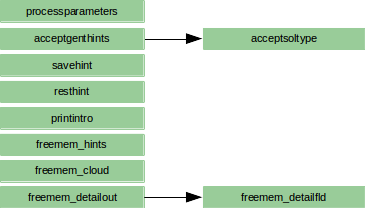
\includegraphics{fig/argumc}
\caption{Function structure of argum.c. The boxes contain function names, and arrows point from a function to the function it calls. Functions are called from left to right, then top to bottom.  Boxes are color-coded as follows:  purple functions are used for eclipse geometry, blue functions are used for transit geometry, green functions are used in both, and red functions are unused at this time.}
\label{fig:argumc}
\end{figure}
\subsubsection{List of Functions Defined in argum.c:}
\function{
int processparameters(int argc, char **argv, struct transit *tr)}
\tgray{Generate the command-line option parser.  Initialize transithint and
populate it's variables based on the command-line arguments.} \newline

\function{
int acceptsoltype(transit\_ray\_solution **sol, char *hname)}
\tgray{Initialize transit ray solution sol. and determine if any of
sol->name matches hname.} \newline

\function{
int acceptgenhints(struct transit *tr)}
\tgray{Set output file names in transit (out, toomuch, and sample).
Initialize transit.sol. Set geometry and detailed output variables in
transit.} \newline

\function{
void savehint(FILE *out, struct transithint *hints)}
\tgray{Saves hints structure.} \newline

\function{
int resthint(FILE *in, struct transithint *hint)}
\tgray{Restore hints structure. The structure needs to have been allocated
before.} \newline

\function{
void printintro()}
\tgray{Print the introductory message.} \newline

\function{
void freemem\_hints(struct transithint *h)}
\tgray{Frees hints structure.} \newline

\function{
void freemem\_cloud(struct extcloud *c)}
\tgray{Free cloud structure. This function is intended to be used when cloud functionality is added but is not used currently.} \newline

\function{
void freemem\_detailout(struct detailout *d)}
\tgray{Driver function to free stored extinction, optical depth, and CIA data.} \newline

\function{
void freemem\_detailfld(struct detailfld *f)}
\tgray{Free a single field of data stored in detailout structure.} \newline


\subsubsection{processparameters:}
\paragraph{Variables Modified:}
\begin{enumerate}[leftmargin=10pt, noitemsep, parsep=0pt, topsep=0ex]
\item[-] Set \ttred{tr.ds.th.verbnoise, tr.ds.th.mass, tr.ds.th.savefiles} (verbosity, abuncance type, and file saving boolean) to defaults.
\item[-] Set \ttred{tr.ds.th.ncross, tr.ds.th.csfile} (number of CS files, CS filenames) from command line arguments/config file.
\item[-] Set \ttred{tr.ds.th.save.ext} (saved extinction grid) from command line arguments/config file.
\item[-] Set \ttred{tr.ds.th.f\_opa} (opacity filename) from command line arguments/config file.
\item[-] Initialize \ttred{tr.ds.th.det.cia, tr.ds.th.det.tau, tr.ds.th.det.ext} (detailed field structures for CIA, optical depth, and/or extinction) if specifed by command line arguments/config file.
\item[-] Fill in the \ttred{tr.ds.th.det} structure values.
\item[-] Set \ttred{tr.ds.th.ethresh} (factor threshold for line profile calculation) from command line arguments/config file.
\item[-] Allocate and set \ttred{tr.ds.th.solname} (ray solution type) from command line arguments/config file.
\item[-] Allocate and set \ttred{tr.ds.th.f\_atm, tr.ds.th.f\_line, tr.ds.th.f\_molfile, \\ tr.ds.th.f\_outmod, tr.ds.th.f\_outsample, tr.ds.th.f\_toomuch, \\ tr.ds.th.f\_outflux,  tr.ds.th.f\_outintens} (input and output filenames) from command line arguments/config file.
\item[-] Set \ttred{tr.ds.th.savefiles} (boolean to save files or not) from command line arguments/config file.
\item[-] Set \ttred{tr.ds.th.p0, tr.ds.th.r0, tr.ds.th.gsurf} (surface pressure, radius, and gravity) from command line arguments/config file.
\item[-] Set \ttred{tr.ds.th.allowrq} (variance from unity allowed in total abundance) from command line arguments/config file.
\item[-] Set \ttred{tr.ds.th.qmol, tr.ds.th.qscale} (species with scale factors, scale factors) from command line arguments/config file.
\item[-] Set \ttred{tr.ds.th.opabreak} (boolean to indicate to the program to break after opacity calculation) from command line arguments/config file.
\item[-] Set \ttred{tr.ds.th.rads.i, tr.ds.th.rads.f, tr.ds.th.rads.d, tr.ds.th.rads.fct} (radius sampling initial value, final value, spacing, and units conversion factor) from command line arguments/config file.
\item[-] Set \ttred{tr.ds.th.wavs.i, tr.ds.th.wavs.f, tr.ds.th.wavs.d, tr.ds.th.wavs.fct} (wavelength sampling initial value, final value, spacing, and units conversion factor) from command line arguments/config file.
\item[-] Set \ttred{tr.ds.th.wns.i, tr.ds.th.wns.f, tr.ds.th.wns.d, tr.ds.th.wns.fct, \\ tr.ds.th.wns.o} (wavenumber sampling initial value, final value, spacing, units conversion factor, and oversampling factor) from command line arguments/config file. Initialize \ttred{tr.ds.th.wns.n} (number of samples) to 0 and \ttred{tr.ds.wns.v} (sampling values) to NULL.
\item[-] Set \ttred{tr.ds.th.temp.i, tr.ds.th.temp.f, tr.ds.th.temp.d} (temperature sampling initial value, final value, and spacing) from command line arguments/config file.
\item[-] Set \ttred{tr.ds.th.timesalpha} (number of half-widths in a Voigt profile) from command line arguments/config file.
\item[-] Set \ttred{tr.ds.th.nDop, tr.ds.th.nLor} (number of Doppler and Lorentz broadening width samples) from command line arguments/config file.
\item[-] Set \ttred{tr.ds.th.dmin, tr.ds.th.dmax, tr.ds.th.lmin, tr.ds.th.lmax} (broadening width sample boundaries) from command line arguments/config file.
\item[-] Set verbosity to 0 if the 'q' command-line argument is given.
\item[-] Set verbosity to specified value if the 'v' command-line argument is given.
\item[-] Set \ttred{tr.ds.th.sg.starrad} (star radius) from command line arguments/config file.
\item[-] Set \ttred{tr.ds.th.sg.smaxis, tr.ds.th.sg.time, tr.ds.th.sg.incl, \\ tr.ds.th.sg.ecc, tr.ds.th.sg.lnode, tr.ds.th.sg.aper} (semimajor axis, phase from eclipse, inclination, eccentricity, longitude of ascending node, argument of pericenter) from command line arguments/config file.
\item[-] Set \ttred{tr.ds.th.sg.smaxisfct, tr.ds.th.sg.timefct, tr.ds.th.sg.inclfct, \\ tr.ds.th.sg.eccfct, tr,.ds.th.sg.lnodefct, tr.ds.th.sg.aperfct} (unit conversion factors for above orbital parameters) from command line arguments/config file.
\item[-] Set \ttred{tr.ds.th.sg.transpplanet} (boolean to set maximum optical depth to toomuch) to True if specified in commmand-line arguments/config file.
\item[-] Set \ttred{tr.ds.th.toomuch} (maximum optical depth to make calculations, above which it is assumed no light transmits) from command line arguments/config file.
\item[-] Set \ttred{tr.ds.th.taulevel} (optical depth integration level) from command line arguments/config file.
\item[-] Set \ttred{tr.ds.th.modlevel} (modulation integration level) from command line arguments/config file.
\item[-] Set \ttred{tr.ds.th.cl.cloudext, tr.ds.th.cl.cloudtop, tr.ds.th.cl.cloudbot} (maximum cloud extinction, initial cloud radius, and final cloud radius) from command line arguments/config file.
\item[-] Set \ttred{tr.ds.th.angles} (intensity angles) from command line arguments/config file.
\end{enumerate}

\paragraph{Walkthrough:}
\begin{enumerate}[leftmargin=10pt, noitemsep, parsep=0pt, topsep=0ex]
\item[-] Set up an enumerated list of all command line arguments, creating a key.
\item[-] Build a structure to identify all command line arguments.
\item[-] Build a configuration paramters structure.
\item[-] Initialize the hint structure, and set all memory to zero.
\item[-] Set up flags, verbosity, abundance units, and whether or not to save files.
\item[-] Set up the detailed output field structures for optical depth, extinction, and CIA.
\item[-] Begin infinite loop:
\begin{enumerate}[leftmargin=10pt, noitemsep, parsep=0pt, topsep=0ex]
\item[-] Call to \ttblue{procopt} from procopt.c to process the command line options. If the option supplies a configuration file, \ttblue{procopt} will parse the file.
\item[-] If \ttblue{procopt} returns -1 (indicating no more command line arguments to process), exit the loop.
\item[-] Handle the returns of \ttblue{procopt} on a case-by-case basis (a case for each command line argument), filling in the hint structure with the specified values. There are too many options to practically list here.
makes the command-line-argument parser, resets the transithint struct, and fill in its variables with default values and command line arguments. 
\end{enumerate} 
\item[-] Call \ttblue{procopt\_free} from procopt.c to free the memory used by \ttblue{procopt}.
\item[-] Return 0 on success.
\end{enumerate}

\subsubsection{acceptsoltype:}
\paragraph{Walkthrough}
\begin{enumerate}[leftmargin=10pt, noitemsep, parsep=0pt, topsep=0ex]
\item[-] Loop over each element in the ray solutions array.
\begin{enumerate}[leftmargin=10pt, noitemsep, parsep=0pt, topsep=0ex]
\item[-] Compare each solution with the given string.
\item[-] If they match, set the solution and return 0.
\end{enumerate}
\item[-] Return -1.
\end{enumerate}

\subsubsection{acceptgenhints:}
\paragraph{Variables Modified}
\begin{enumerate}[leftmargin=10pt, noitemsep, parsep=0pt, topsep=0ex]
\item[-] Copy \ttred{tr.f\_outmod} from {\tt th.f\_outmod} or default (modulation
  output filename).
\item[-] Copy \ttred{tr.f\_outflux} from {\tt th\_outflux} or default (flux output filename).
\item[-] Copy \ttred{tr.f\_toomuch, tr.f\_outsample, tr.outintens} from {\tt
    th.f\_toomuch, \\ th.f\_outsample, th.f\_outintens} (maximum optical depth,
  sampling output, and intensity output filenames).
\item[-] Copy \ttred{tr.ds.det} from {\tt th.det} (detailed output structure).
\item[-] Copy \ttred{tr.timesalpha} from {\tt th.timesalpha} (Voigt profile width).
\item[-] Copy \ttred{tr.opabreak} from {\tt th.opabreak}.
\item[-] Set \ttred{tr.interpflag} to SAMP\_LINEAR or SAMP\_SPLINE depending on {\tt tr.fl} (flag).
\item[-] Copy \ttred{tr.r0} from {\tt th.r0} (reference radius).
\item[-] Copy \ttred{tr.p0} from {\tt th.p0} (reference radius).
\item[-] Copy \ttred{tr.gsurf} from {\tt th.gsurf} (surface gravity).
\item[-] Call \ttblue{parseArray} from iomisc.c to copy  \ttred{tr.qscale} from {\tt th.qscale} and set \ttred{tr.nqmol} to the size of {\tt th.qscale}. If {\tt th.qscale} was not given, set \ttred{tr.nqmol} to 0.
\end{enumerate}

\paragraph{Walkthrough:}
\begin{enumerate}[leftmargin=10pt, noitemsep, parsep=0pt, topsep=0ex]
\item[-] Set output filenames for modulation, flux, radius where maximum tau was reached, sampling, and intensity from hint structure.
\item[-] Set molecular filename from hint structure.
\item[-] Call to \ttblue{acceptsoltype} from argum.c to get the solution type. Raise an error if an invalid type was provided, and exit program.
\item[-] Call to \ttblue{setgeomhint} from geometry.c to set hinted geometry information.
\item[-] Copy the hinted detailed output structure.
\item[-] Check that the given number of alpha units in Voigt profile width is more than 1. If not, raise an error and return -1.
\item[-] Set the number of alpha units in Voigt profile width.
\item[-] Check that the transition line strength threshold is positive. If not, raise an error and return -1.
\item[-] Call \ttblue{transitacceptflag} (defined in transit.h) to pass atmospheric flags into the transit structure.
\item[-] Set the flag to break {\tt transit} after the opacity grid has been calculated from the hint structure.
\item[-] Set the interpolation function flag. Raise an error if invalid function specified.
\item[-] Raise an error and return -1 if the specified reference radius is negative.
\item[-] Set the reference radius from the hint structure.
\item[-] Raise an error and return -1 if the specified reference pressure is negative.
\item[-] Set the reference pressure from the hint structure.
\item[-] Raise an error and return -1 if the specified surface gravity is negative.
\item[-] Set the surface gravity from the hint structure.
\item[-] If abundance scale factors were specified:
\begin{enumerate}[leftmargin=10pt, noitemsep, parsep=0pt, topsep=0ex]
\item[-] Call \ttblue{parseArray} from iomisc.c to set the abundance scale factors from the hint structure and set the number of scale factors.
\item[-] If the number of molecules with scale factors does not match the size of the scale factors array, raise an error.
\end{enumerate}
\item[-] Otherwise, set the number of scale factors to 0.
\item[-] Return 0 on success.
\end{enumerate}

\subsubsection{savehint:}
\paragraph{Walkthrough}
\begin{enumerate}[leftmargin=10pt, noitemsep, parsep=0pt, topsep=0ex]
\item[-] Write the hint structure to file.
\item[-] Call to \ttblue{savestr} from transitstd.c to write input and output filenames, in binary, to file (atmosphere, TLI, CS, modulation, flux, intensity, radius where maximum tau was reached, and sampling files). Write the solution name to file.
\item[-] Call to \ttblue{savesample\_arr} from makesample.c to save the radius, wavelength, wavenumber, and impact parameter sampling to file.
\end{enumerate}

\subsubsection{resthint:}
\paragraph{Variables Modified}
\begin{enumerate}[leftmargin=10pt, noitemsep, parsep=0pt, topsep=0ex]
\item[-] Restore \ttred{tr.ds.th.f\_atm, tr.ds.th.f\_line, tr.ds.th.f\_outmod,\\ tr.ds.th.f\_outflux,  tr.ds.th.f\_outintens, tr.ds.th.f\_toomuch, \\ tr.ds.th.f\_outsample, tr.ds.th.solname,  tr.ds.th.csfile} from file.
\item[-] Restore \ttred{tr.ds.th.rads, tr.ds.th.wavs, tr.ds.th.wns, tr.ds.th.ips} from file.
\end{enumerate}

\paragraph{Walkthrough}
\begin{enumerate}[leftmargin=10pt, noitemsep, parsep=0pt, topsep=0ex]
\item[-] Restore the main hint structure from file.
\item[-] If reading the file returns an error, return the error. Otherwise, increment the function result by the number of elements read from file.
\item[-] Call \ttblue{reststr} from transitstd.c to restore the strings in the hint structure.
\item[-] Call \ttblue{restsample\_arr} from makesample.c to restore the arrays in the hint structure.
\item[-] Return the number of elements read from the file.
\end{enumerate}

\subsubsection{freemem\_hints:}
\paragraph{Variables Modified}
\begin{enumerate}[leftmargin=10pt, noitemsep, parsep=0pt, topsep=0ex]
\item[-] Free \ttred{tr.ds.th.f\_atm, tr.ds.th.f\_line, tr.ds.th.f\_outmod, tr.ds.th.f\_outflux, \\ tr.ds.th.f\_outintens, tr.ds.th.f\_toomuch, tr.ds.th.f\_outsample, \\ tr.ds.th.f\_molfile, tr.ds.th.solname, tr.ds.th.csfile}.
\end{enumerate}

\paragraph{Walkthrough}
\begin{enumerate}[leftmargin=10pt, noitemsep, parsep=0pt, topsep=0ex]
\item[-] Free all filenames in the hint structure.
\item[-] Free the solution name.
\item[-] Call to \ttblue{freemem\_samp} from makesample.c to free the hinted sampling for radius, wavelength, wavenumber, and impact parameter.
\item[-] Call to \ttblue{freemem\_cloud} from argum.c to free hinted cloud info.
\item[-] Call to \ttblue{freemem\_detailout} from argum.c to free hinted detailed output structure.
\end{enumerate}

\newpage
\subsection{geometry.c:}
This file contains routines which handle the hinted geometry parameters and make calculations regarding the geometry of the transit or eclipse.
\subsubsection{List of Functions Defined in geometry.c:}
\function{
int setgeomhint(struct transit *tr)}
\tgray{Set transit geometry variables (tr.ds.sg) from hint or default
variables.} \newline

\function{
int setgeom(struct geometry *sg, double time, long *flags)}
\tgray{Set $x$ and $y$ geometry variables (coordinates of the planet relative to the star)}. \newline

\function{
inline PREC\_RES starvariation(double x, double y, double radius)}
\tgray{Evaluate if $x\sp{2} + y\sp{2} > {\rm radius}\sp{2}$. Return 0 if so. Otherwise return 1.} \newline

\subsubsection{setgeomhint}
\paragraph{Modified}
\begin{enumerate}[leftmargin=10pt, noitemsep, parsep=0pt, topsep=0ex]
\item[-] Copy {\tt th.sg.transpplanet} into \ttred{tr.ds.sg.transpplanet}.
\item[-] Set all \ttred{tr.ds.sg} variables except {\tt
    tr.ds.sg.x} and {\tt tr.ds.sg.y} from {\tt th.sg}. If a hinted value is not given, set them to default values.
\item[-] Update \ttred{tr.pi} to account for {\tt TRPI\_GEOMETRYHINT}.
\end{enumerate}

\paragraph{Walkthrough}
\begin{enumerate}[leftmargin=10pt, noitemsep, parsep=0pt, topsep=0ex]
\item[-] Copy hinted transpplanet into the transit structure. This is a boolean which, if true, sets the maximum optical depth to toomuch.
\item[-] Set all variables in the geometry structure from the hinted structure ({\tt tr.ds.th.sg}) except X and Y values (coordinates of planet relative to the star). If no hinted variable is given, the variables are set to a default value.
\item[-] Update the progress indicator to account for {\tt TRPI\_GEOMETRYHINT}.
\item[-] Return 0 on success.
\end{enumerate}

\subsubsection{setgeom}
\paragraph{Modified}
\begin{enumerate}[leftmargin=10pt, noitemsep, parsep=0pt, topsep=0ex]
\item[-] Calculate \ttred{sg.x, sg.y} by solving the Kepler equation.
\item[-] Update \ttred{tr.pi} to account for {\tt TRPI\_GEOMETRY}.
\end{enumerate}

\paragraph{Walkthrough}
\begin{enumerate}[leftmargin=10pt, noitemsep, parsep=0pt, topsep=0ex]
\item[-] Calculate semi-major axis, eccentricity, inclination, observation time, and stellar mass in cgs units.
\item[-] Set the precision limit for the square of the eccentric anomaly.
\item[-] Calculate mean motion (orbital angular frequency).
\item[-] Set the approximate eccentric anomaly and calculate the eccentric anomaly
\item[-] While the square of the difference between the eccentric anomaly approximation and the eccentric anomaly is greater than the precision limit, set the approximation equal to the eccentric anomaly and recalculate the eccentric anomaly at time t. When the loops exits, the eccentric anomaly at time t will have been calculated.
\item[-] Calculate orbital parameters.
\item[-] Calculate the position of the planet relative to the center of the star ({\tt sg.x, sg.y}).
\item[-] Update the progress indicator to account for {\tt TRPI\_GEOMETRY}.
\item[-] Return 0 on success.
\end{enumerate}

\subsubsection{starvariation}
\paragraph{Walkthrough}
\begin{enumerate}[leftmargin=10pt, noitemsep, parsep=0pt, topsep=0ex]
\item[-] Return 0 if position (x, y) is not within a circle of given radius.
\item[-] Return 1 otherwise.
\end{enumerate}

\newpage
\subsection{readlineinfo.c:}
This file is concerned with reading TLI files produced by the {\tt pylineread} program. Only binary TLI files are accepted. Functions \ttblue{saveline, main} are not currently used in {\tt transit}. Figure \ref{fig:readlineinfoc} shows this function structure.

\begin{figure}
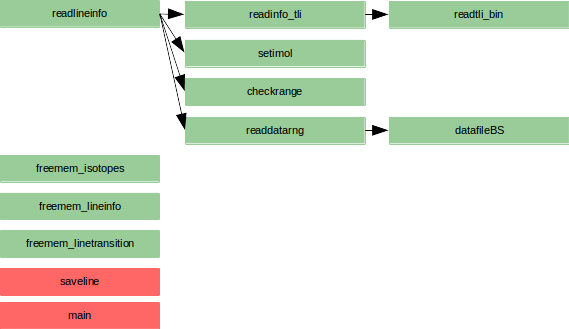
\includegraphics{fig/readlineinfoc}
\caption{Function structure of readlineinfo.c. The boxes contain function names, and arrows point from a function to the function it calls. Functions are called from left to right, then top to bottom.  Boxes are color-coded as follows:  purple functions are used for eclipse geometry, blue functions are used for transit geometry, green functions are used in both, and red functions are unused at this time.}
\label{fig:readlineinfoc}
\end{figure}

\subsubsection{List of Functions Defined in readlineinfo.c:}
\function{
static inline void datafileBS(&FILE *fp, PREC\_NREC offs, PREC\_LNDATA target,
                           \\ &PREC\_NREC *resultp, int reclength, int up)}
\tgray{Do a binary search in file pointed by 'fp' between 'off' and
'off+nfields' looking for 'target' as the first item of a record
of length 'reclength', result index (with respect to offs) is
stored in 'resultp'.} \newline

\function{
int readlineinfo(struct transit *tr)}
\tgray{Driver function to read TLI: read isotopes info, check margin and
ranges, and read line transition information.} \newline

\function{
int readinfo\_tli(struct transit *tr, struct lineinfo *li)}
\tgray{Check if a TLI file exists.  Check that machine formating is compatible
with lineread.  Determine if TLI is ASCII or binary.  Read either
ASCII or binary TLI file. Declare line\_transition.} \newline

\function{
int readtli\_bin(FILE *fp, struct transit *tr, struct lineinfo *li)}
\tgray{Read initial and final wavelength limits and number of databases.
Allocate pointers to database, and isotope arrays.
Get databases info: names, number of temperatures, temperatures, number
of isotopes, isotope names and masses, partition function, and
cross sections. Get cumulative number of isotopes.} \newline

\function{
int setimol(struct transit *tr)}
\tgray{Set each isotope's molecular identifier number.} \newline

\function{
int checkrange(struct transit *tr, struct lineinfo *li)}
\tgray{Initialize wavelength sample struct.  Set margin.  
Set initial and final wavelengths to use.  
Check that margin leaves a non-zero wavelength range.} \newline

\function{
int readdatarng(struct transit *tr, struct lineinfo *li)}
\tgray{Read and store the line transition info (central wavelength, isotope
ID, lowE, log(gf)) into lineinfo.  Return the number of lines read.} \newline

\function{
int freemem\_isotopes(struct isotopes *iso, long *pi)}
\tgray{Frees isotope structure.} \newline

\function{
int freemem\_linetransition(struct line\_transition *lt, long *pi)}
\tgray{Frees line transition data.} \newline

\function{
int freemem\_lineinfo(struct lineinfo *li, long *pi)}
\tgray{Frees line transition info.} \newline

\function{
void saveline(FILE *fp, struct lineinfo *li)}
\tgray{Saves line information.} \newline

\function{
int main(int argc, char **argv)}
\tgray{For debugging only.} \newline

\subsubsection{readlineinfo:}
\paragraph{Variables Modified}
\begin{enumerate}[leftmargin=10pt, noitemsep, parsep=0pt, topsep=0ex]
\item[-] Reset \ttred{tr.ds.li, tr.ds.iso} (lineinfo and
  isotopes structures).
\item[-] Set \ttred{tr.ds.li.tmin, tr.ds.li.tmax} (min and max temperatures in TLI files).
\item[-] If an opacity file exists, update \ttred{tr.pi} to account for TRPI\_READINFO and TRPI\_READDATA.
\end{enumerate}

\paragraph{Walkthrough}
\begin{enumerate}[leftmargin=10pt, noitemsep, parsep=0pt, topsep=0ex]
\item[-] Reset line information and isotopes structures.
\item[-] Set min and max allowed temperatures in TLI files.  
\item[-] Call \ttblue{readinfo\_tli} to check if TLI file exists, open it, and get header information (all info exept line transitions). 
\item[-] If \ttblue{readinfo\_tli} was successful, call \ttblue{checkrange} to check the range of the hinted values against the range of wavelengths in the TLI file.
\item[-] Call \ttblue{setimol} to set the molecular index of each isotope. 
\item[-] Check if an opacity file exists. If not, and \ttblue{checkrange} was successful, call \ttblue{readdatarng} to read the TLI file data. Otherwise, skip reading the TLI file and update the progress indicator to allow the program to continue.
\item[-] Return 0 on success.
\end{enumerate}


\subsubsection{readinfo\_tli:}
\paragraph{Variables Modified}
\begin{enumerate}[leftmargin=10pt, noitemsep, parsep=0pt, topsep=0ex]
\item[-] Set \ttred{tr.f\_line} from {\tt th.f\_line} if file
  exists and could be opened (TLI filename).
\item[-] Set \ttred{tr.fp\_line} (pointer to TLI file).
\item[-] Declare \ttred{tr.ds.li.lt}.
\item[-] Set \ttred{tr.ds.li.lt.wfct, tr.ds.li.lt.efct} from
  default values (line-transition wavelength and lowE units factor).
\item[-] Update \ttred{tr.pi} to include {\tt TRPI\_READINFO}.
\end{enumerate}

\paragraph{Walkthrough}
\begin{enumerate}[leftmargin=10pt, noitemsep, parsep=0pt, topsep=0ex]
\item[-] Declare a union variable which is used to determine endianness compatibility.
\item[-] Check that a TLI file name was given. If not, raise an error and return -2.
\item[-] Check if TLI file exists. If not, raise an error and return -1.
\item[-] Set the TLI file name and file pointer from hint structure.
\item[-] Read the first four bytes of the TLI file into the union variable.
\item[-] Call to \ttblue{readtli\_bin} to read the binary TLI file. Raise an error and return -6 if \ttblue{readtli\_bin} returns an error.
\item[-] Set the wavelength and lowE units conversion factor for line transitions.
\item[-] Update the progress indicator.
\item[-] Return -1 on success.
\end{enumerate}

\subsubsection{readtli\_bin:}
\paragraph{Variables Modified}
\begin{enumerate}[leftmargin=10pt, noitemsep, parsep=0pt, topsep=0ex]
\item[-] Set \ttred{tr.ds.li.tli\_ver, tr.ds.li.lr\_ver,
    tr.ds.li.lr\_rev} from TLI file (lineinfo TLI version, lineinfo
  version and revision).
\item[-] Allocate \ttred{tr.ds.iso.db} (database structures for each isotope).
\item[-] Allocate \ttred{tr.ds.li.db} (database structures for temperature information).
\item[-] Allocate \ttred{tr.ds.iso.isof} (structure for fixed isotope information).
\item[-] Allocate \ttred{tr.ds.li.isov} (structure for variable isotope information).
\item[-] Allocate \ttred{tr.ds.iso.isoratio} (isotope abundance ratio).
\item[-] Allocate \ttred{tr.ds.iso.db.n, tr.ds.iso.db.molname} (database name and molecule name) for each database.
\item[-] Set \ttred{tr.ds.li.db.t, tr.ds.iso.db.i} (number of temperatures and number of isotopes) for each database.
\item[-] Allocate \ttred{tr.ds.li.db.T} (temperature points in TLI file) for each database and set from the TLI file.
\item[-] Reallocate \ttred{tr.ds.li.isov, tr.ds.iso.isof, tr.ds.iso.isoration} to account for new isotopes.
\item[-] Allocate \ttred{tr.ds.li.isov.z} (partition function).
\item[-] Set \ttred{tr.ds.iso.isof.d} (database index of the isotope) for each isotope.
\item[-] Allocate and set \ttred{tr.ds.iso.isof.n} (isotope name) for each isotope.
\item[-] Set \ttred{tr.ds.iso.isof.m} (mass) for each isotope.
\item[-] Set \ttred{tr.ds.iso.isoratio} (isotopic ratio) for each isotope.
\item[-] Set \ttred{tr.ds.li.isov.z} (partition function) for each isotope.
\item[-] Set \ttred{tr.ds.li.isov.n} (partition function array length) for each isotope.
\item[-] Set \ttred{tr.ds.iso.db.s} (index of the first isotope) for each database (species).
\item[-] Set \ttred{tr.ds.li.ni, tr.ds.iso.n\_i} (number of isotopes).
\item[-] Set \ttred{tr.ds.li.ndb, tr.ds.iso.n\_db} (number of databases).
\item[-] Set \ttred{tr.ds.li.iniw, tr.ds.li.finw} (initial and final wavelength).
\item[-] Set \ttred{tr.ds.li.endinfo} (position of beginning of transition data).
\item[-] Allocate \ttred{tr.ds.iso.isov} (structures for isotopes' variable data).
\end{enumerate}

\paragraph{Walkthrough}
\begin{enumerate}[leftmargin=10pt, noitemsep, parsep=0pt, topsep=0ex]
\item[-] Read the TLI version, lineread version, and lineread revision number from the TLI file.
\item[-] Check that the TLI version is compatible with the transit version. If not, raise an error.
\item[-] Read the initial wavelength, final wavelength, and number of databases from the TLI file.
\item[-] Allocate structures for databases for each isotope.
\item[-] Allocate structures for fixed and variable isotope data.
\item[-] Allocate isotopic abundance ratios.
\item[-] Set max and min allowed temperatures.
\item[-] Loop over each database (each species):
\begin{enumerate}[leftmargin=10pt, noitemsep, parsep=0pt, topsep=0ex]
\item[-] Read database name length, allocate space for the name, and read the name from the TLI file.
\item[-] Read molecule name length, allocate space for the name, and read the name from the TLI file.
\item[-] Read and set the number of temperatures and number of isotopes.
\item[-] Allocate array for the temperatures and read from the file.
\item[-] Reallocate variable isotope data structures, fixed isotope data structures, and isotopic abundance ratio to account for new isotopes.
\item[-] Allocate array for partition function data.
\item[-] Loop over each isotope:
\begin{enumerate}[leftmargin=10pt, noitemsep, parsep=0pt, topsep=0ex]
\item[-] Set isotope's database index number.
\item[-] Read isotope name length, allocate space for the name, and read the name from the TLI file.
\item[-] Read isotope mass and isotopic ratio from the TLI file.
\end{enumerate}
\item[-] Set the index of the first isotope in this isotope.
\item[-] Increment the number of isotopes by the number of isotopes in this database.
\end{enumerate}
\item[-] Set the number of total isotopes, number of databases, position of the first transition in the TLI file, initial wavelength, final wavelength, and number of databases (in both the line transition and isotopes structures).
\item[-] Allocate structures for isotopes' variables data.
\item[-] Return 0 on success.
\end{enumerate}


\subsubsection{checkrange:}
\paragraph{Walkthrough}
\begin{enumerate}[leftmargin=10pt, noitemsep, parsep=0pt, topsep=0ex]
\item[-] Calculate wavelength limits in cgs units.
\item[-] If the final wavelength given is less than the minimum wavelength in the database, return -3.
\item[-] If the final wavelength given is greater than the maximum wavelength in the database, raise a warning.
\item[-] If the initial wavelength given is greater than the maximum wavelength in the database, return -2.
\item[-] If the initial wavelength given is less than the minimumn wavelength in the database, raise a warning.
\item[-] Return the result (0 on success).
\end{enumerate}

\subsubsection{readdatarng:}
\paragraph{Variables Modified}
\begin{enumerate}[leftmargin=10pt, noitemsep, parsep=0pt, topsep=0ex]
\item[-] Allocate \ttred{tr.ds.li.lt.wl, tr.ds.li.lt.isoid,
    tr.ds.li.lt.gf, tr.ds.li.lt.elow} (line-transition's wavelength,
  isotope ID, gf, and lower state energy).
\item[-] Set \ttred{tr.ds.li.lt.wl, tr.ds.li.lt.isoid, tr.ds.li.lt.gf, tr.ds.li.lt.elow} from read TLI values.
\item[-] Set \ttred{tr.ds.li.n\_l} (Number of lines read from TLI).
\item[-] Update \ttred{tr.pi to} include {\tt TRPI\_READDATA}.
\end{enumerate}

\paragraph{Walkthrough} 
\begin{enumerate}[leftmargin=10pt, noitemsep, parsep=0pt, topsep=0ex]
\item[-] Call to \ttblue{fileexistopen} from iomisc.c to open the TLI file. Return 0 if no file was given. If the file exists but cannot be opened, return -1.
\item[-] Check if the file is 'seekable'. If not, raise an error and return -2.
\item[-] Move the file pointer to the beginning of the transition data.
\item[-] Read the number of transitions from the TLI file.
\item[-] Read the number of isotopes from the TLI file.
\item[-] Read the number of transitions per isotope from the TLI file.
\item[-] Loop over subsequent wavelength entries to check that they are greater than the final wavelength. If not, increment the index of the final wavelength until the condition is true.
\item[-] Store the number of lines.
\item[-] Allocate arrays for line transition's oscillator strength, central wavelength, isotope ID, and lower-state energy.
\item[-] Check for allocation errors. Raise an error if any of the allocations failed.
\item[-] Set the starting location for wavlengths, isotope IDs, lower-state energy, and oscillator strength.
\item[-] Loop over each isotope:
\begin{enumerate}[leftmargin=10pt, noitemsep, parsep=0pt, topsep=0ex]
\item[-] Call to \ttblue{datafileBS} to find the index of the first transition to be read.
\item[-] Call to \ttblue{datafileBS} to find the index of the last transition to be read.
\item[-] Move file pointer to the beginning of the wavelength info and read into the allocated array. Do the same for isotope IDs, lower-state energy, and oscillator strength (gf).
\item[-] Increment the number of lines read.
\item[-] Move the wavelength offset to the next isotope.
\end{enumerate}
\item[-] Reallocate the central wavelength, isotope ID, lower-state energy, and osciallator strength arrays to the correct size.
\item[-] Close the file.
\item[-] Update progress indicator.
\item[-] Return the number of lines read.
\end{enumerate}

\subsubsection{datafileBS:}
\paragraph{Walkthrough}
\begin{enumerate}[leftmargin=10pt, noitemsep, parsep=0pt, topsep=0ex]
\item[-] Set the index of the end of the search range to one less than the number of fields to search. Set the index of the beginning of the range to 0.
\item[-] Perform binary search. While the difference between the beginning and end indices is greater than 1:
\begin{enumerate}[leftmargin=10pt, noitemsep, parsep=0pt, topsep=0ex]
\item[-] Set the result index to the middle of the search range.
\item[-] Move the file pointer to the result index.
\item[-] Read the value at that point.
\item[-] If the target value is greater than the read value, move the beginning of the search range up to the result index. Otherwise, move then end of the search range to the result index.
\end{enumerate}
\item[-] Perform a linear search through entries above or below that found by the binary search depending on the flag passed.
\item[-] Set the result index to the beginning index of the search range.
\item[-] Move the file pointer to this point.
\item[-] Read the value at that point in the file. 
\end{enumerate}

\subsubsection{setimol:}
\paragraph{Variables Modified}
\begin{enumerate}[leftmargin=10pt, noitemsep, parsep=0pt, topsep=0ex]
\item[-] Allocate and fill \ttred{tr.ds.iso.imol} (molecular indices array).
\end{enumerate}

\paragraph{Walkthrough}
\begin{enumerate}[leftmargin=10pt, noitemsep, parsep=0pt, topsep=0ex]
\item[-] Return 0 if there are no isotopes.
\item[-] Allocate molecular indices array.
\item[-] Loop over isotopes:
\begin{enumerate}[leftmargin=10pt, noitemsep, parsep=0pt, topsep=0ex]
\item[-] Call to \ttred{findstring} from iomisc.c to find the index of the molecule name in the list of isotope database molecule names.
\item[-] If the found molecule is not already in the molecular indices array, increment the total number of molecules.
\end{enumerate}
\item[-] Return 0 on success.
\end{enumerate}

\newpage
\subsection{readatm.c:}
This file contains functions which read the atmospheric file. \ttblue{telldefaults} is currently unused. Figure \ref{fig:readatmc} shows the function structure.

\begin{figure}
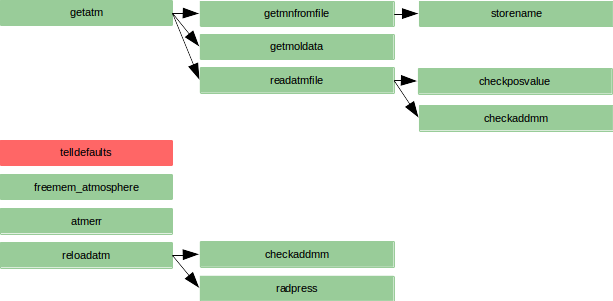
\includegraphics{fig/readatmc}
\caption{Function structure of readatm.c. The boxes contain function names, and arrows point from a function to the function it calls. Functions are called from left to right, then top to bottom.  Boxes are color-coded as follows:  purple functions are used for eclipse geometry, blue functions are used for transit geometry, green functions are used in both, and red functions are unused at this time.}
\label{fig:readatmc}
\end{figure}

\subsubsection{List of Functions Defined in readatm.c:}
\function{
int getatm(struct transit *tr)}
Initialize ds.at (atm\_data).  Set abundance mass and allowrq parameters.
Check existence, open, and set pointer to atmosphere file.
Get keyword variables from atm file (list of isotopes among others).
Get temperature and isotopes abundances per radius from atm file. \newline

\function{
double checkaddmm(&double *mm, PREC\_NREC r, prop\_isov *isov, prop\_isof *isof,
               \\ &int n, \_Bool mass, enum isodo *isodo)}
Compute the mean molecular mass, check that sum of abundances
is no bigger than 1, and return it. \newline

\function{
void telldefaults(struct isotopes *iso, struct atm\_data *at)}
Tell defaults when only one radius is being selected. \newline

\function{
int freemem\_atmosphere(struct atm\_data *at, long *pi)}
Free memory from the atmosphere structure. \newline

\function{
void storename(struct atm\_data *at, char *line)}
Store info about the atmosphere file. \newline

\function{
static void atmerr(int max, char *file, int line)}
Print error message when a line of the file is longer than the max characters. \newline

\function{
static void invalidfield(char *line, int nmb, int fld, char *fldn)}
Print an error message when a field with transition info is invalid. \newline

\function{
static inline void checkposvalue(PREC\_RES val, int field, long line)}
Chack that a value is positive, and raise an error if it is not. \newline

\function{
int getmnfromfile(FILE *fp, struct atm\_data *at, struct transit *tr)}
Get keyword variables from atmosphere file (mass/number abundance bool;
zero-radius offset; radius, temperature, and pressure units factor;
atmfile name/info; list isotopes; list of proportional-abundance isotopes).
Store molecules and proportional isotopes in atm\_data struct.
Determine which linedb isotope corresponds to such atm\_data isotope.
Solve non-matched linedb isotope cases.
Put all non-ignore isotopes in transit.ds.iso structure. \newline

\function{
int readatmfile(FILE *fp, struct transit *tr, struct atm\_data *at, \\ prop\_samp *rads, int nrad)}
Read and store radius, pressure, and temperature from file.
Read abundances for each (non other-factor) isotope.
Sum fractional abundances. Calculate ramaining (other-factor) abundances.
Calculate mean molecular mass per radius.
Calculate densities per isotope at each radius. \newline

\function{
void getmoldata(struct atm\_data *at, struct molecules *mol, char *filename)}
Read and store non-layer-dependent molecular data (mass, radius, ID)
and store in mol struct. \newline

\function{
int reloadatm(struct transit *tr, double *input)}
Reload data from array into transit's atm structure.\newline

\function{
int radpress(double g, double p0, double r0, double *temp, double *mu,\\ double *pressure, double *radius, intnlayer, double rfct)}
Recalculate radius array according to hydrostatic pressure, and find the radial location of the reference pressure.

\subsubsection{getatm:}
\paragraph{Variables Modified:}
\begin{enumerate}[leftmargin=10pt, noitemsep, parsep=0pt, topsep=0ex]
\item[-] Initialize \ttred{tr.ds.at, tr.ds.mol}  (atm\_data, molecules).
\item[-] Set \ttred{tr.ds.at.mass} from {\tt th.mass} (mass or
  number abundance bool).
\item[-] Set \ttred{tr.allowrq} from {\tt th.allowrq} (minimum
  allowed sum of abundances).
\item[-] Set \ttred{tr.fp\_atm} from {\tt th.f\_atm} if {\tt th.f\_atm} exists and can be
  opened (atmosphere file pointer).
\item[-] Set \ttred{tr.f\_atm} (atmosphere file name).
\item[-] Set \ttred{tr.ds.at.atm.tfct, tr.ds.at.atm.pfct} from
  default values (temperature and pressure unit factors).
\item[-] Allocate \ttred{tr.ds.at.rads.v, tr.ds.at.atm.t,
    tr.ds.at.atm.p} (radius, temperature and pressure array).
\item[-] Allocate \ttred{tr.ds.mol.nmol, tr.ds.mol.ID, tr.ds.mol.mass, tr.ds.mol.radius, \\ tr.ds.mol.molec} (number of molecules, molecular IDs, molecular masses, molecular radii, and molecular properties).
\item[-] Allocate \ttred{tr.ds.at.molec, tr.ds.at.mm, tr.ds.at.molec.d, tr.ds.at.molec.q} (molecular properties substructure, mean molecular mass, molecular density, molecular abundance) and set \ttred{tr.ds.at.molec.n} (size of radius sampling)
\item[-] Set \ttred{tr.ds.at.rads.i, tr.ds.at.rads.f, tr.ds.at.rads.o,
    tr.ds.at.rads.d} (radius sampling initial value, final value,
  oversampling, and spacing).
 \item[-] Update \ttred{tr.pi} to account for {\tt TRPI\_GETATM}.
\end{enumerate}

\paragraph{Walkthrough:}
\begin{enumerate}[leftmargin=10pt, noitemsep, parsep=0pt, topsep=0ex]
\item[-] Initialize atmosphere and molecular structures by setting memory to 0.
\item[-] Copy mass boolean from the transithint structure. This boolean indicates whether abundances are in units mass or number.
\item[-] Copy abundance exactness number from transithint structure. This number determines if an error is raised when the sum of the abundances does not equal one.
\item[-] If the atmospheric file was not specified, raise an error and return -1.
\item[-] If the atmospheric file is specified, exists, and can be opened, set the file pointer and file name.
\item[-] Allocate radius sampling values, temperature, and pressure arrays.
\item[-] Call \ttblue{getmnfromfile} from readatm.c to get keyword variables from the atmospheric file. Raise an error if the atmospheric file contains less than 1 line read.
\item[-] Allocate molecular structure variables (number of molecules, molecular ID, molecular masses, molecular radii, and molecular properties substructure).
\item[-] Call \ttblue{getmoldata} to get molecular data from the molecules file.
\item[-] Allocate molecular properties substructure of atmospheric data structure, mean molecular mass, molecular density, and molecular density. Set number of elements.
\item[-] Call to \ttblue{readatmfile} to read per-radius isotopic abundances, temperatures and set number a radius layers.
\item[-] Close the file.
\item[-] Set the radius sampling initial value, final value, oversampling, and spacing.
\item[-] Update progress indicator to show \ttblue{getatm} has been run.
\item[-] Return 0 on success.
\end{enumerate}

\subsubsection{checkaddmm:}
\paragraph{Walkthrough}
\begin{enumerate}[leftmargin=10pt, noitemsep, parsep=0pt, topsep=0ex]
\item[-] Raise an error if given radius layer is beyond the allocated radius layers.
\item[-] Compute mean molecular mass and sum of abundances.
\item[-] If the sum of abundances is more than 0.1\% over unity, raise a warning.
\item[-] Return the sum of the abundances.
\end{enumerate}

\subsubsection{getmnfromfile:}
\paragraph{Variables Modified}
\begin{enumerate}[leftmargin=10pt, noitemsep, parsep=0pt, topsep=0ex]
\item[-] Set \ttred{tr.ds.at.begline} (line where radius-dependent info begins) to 0.
\item[-] Allocate and fill out \ttred{tr.ds.mol.name} (molecules' names).
\item[-] Set \ttred{tr.ds.at.mass} according to the atmospheric file.
\item[-] Set \ttred{tr.ds.at.info} according to the atmospheric file.
\item[-] Set \ttred{tr.ds.at.begpos} (position of the beginning of data).
\end{enumerate}

\comment{\paragraph{Walkthrough}
\begin{enumerate}[leftmargin=10pt, noitemsep, parsep=0pt, topsep=0ex]
\item[-] Begin infinite loop.
\begin{enumerate}[leftmargin=10pt, noitemsep, parsep=0pt, topsep=0ex]
\item[-] Call \ttblue{fgetupto\_err} from iomisc.c to read given file character by character and place into given string. Each character is treated on a case-by-case basis:
\begin{enumerate}[leftmargin=10pt, noitemsep, parsep=0pt, topsep=0ex]
\item[-] When a '\textbackslash n' is encountered, continue to the next line.
\item[-] When a '#' character is encountered:
\begin{enumerate}[leftmargin=10pt, noitemsep, parsep=0pt, topsep=0ex]
\item[-] Call \ttblue{getname} from iomisc.c to read the following characters until reaching a blank space, end of line, or end of file, and store those characters in the given string (keyword).
\item[-] If the keyword is SPECIES:
\begin{enumerate}[leftmargin=10pt, noitemsep, parsep=0pt, topsep=0ex]
\item[-] Call \ttblue{fgetupto\_err} from iomisc.c to go to the next line.
\item[-] Call \ttblue{countfields} from iomisc.c to count the number of words in this line. This is the number of molecules.
\item[-] Allocate array for molecules' names.
\item[-] Loop over each molecule. Call \ttblue{getname} from iomisc.c to read the next molecule name and store in the array. Call \ttblue{nextfield} from iomisc.c to move the file pointer to the beginning of the next word (next molecule name).
\item[-] Continue reading the file.
\end{enumerate}
\end{enumerate}
\item[-] When a '0' character is encountered, raise an error that the end of the file has been reached before data was read.
\item[-] When a 'q' character is encountered:
\begin{enumerate}[leftmargin=10pt, noitemsep, parsep=0pt, topsep=0ex]
\item[-] Skip past all blank spaces.
\item[-] If a 'n' character is after the 'q' character, set the mass boolean to false, indicating abundance is a mixing ratio. If a 'm' character is after the 'q' character, set the mass boolean to true, indicating abundance is a mass mixing ratio. Otherwise, raise an error and break.
\item[-] Continue reading the file.
\end{enumerate}
\item[-] When a 'z' character is encountered, set the zero radius value to the following number.
\item[-] When a 'u' character is encountered:
\begin{enumerate}[leftmargin=10pt, noitemsep, parsep=0pt, topsep=0ex]
\item[-] If the next character is a 'r', set the radius sampling factor to the following number.
\item[-] If the next character is a 'p', set the pressure factor to the following number.
\item[-] If the next character is a 't', set the temperature factor to the following number.
\item[-] Otherwise, raise an error and exit.
\end{enumerate}
\item[-] When a 'n' character is encountered, call \ttblue{storename} from readatm.c to store the following string as the file name/label.
\item[-] If none of these characters are encountered, break case switch and infinite loop.
\end{enumerate}
\item[-] Set total number of molecules in the atmosphere.
\item[-] If the number of species scale factors is greater than 0:
\begin{enumerate}[leftmargin=10pt, noitemsep, parsep=0pt, topsep=0ex]
\item[-] Allocate array for species with scale factors.
\item[-] Loop over each species. Set the species with scale factor entry to -1. Compare each species with molecular names and if they are the same, fill in the species with scale factor entry, such that all that are present are named, and those not present are listed as -1.
\end{enumerate}
\item[-] If no molecules were defined, raise an error.
\item[-] Set the position in the file of the beginning of data.
\item[-] Return the line where radius-dependent info begins.
\end{enumerate}
}

\subsubsection{readatmfile:}
\paragraph{Variables Modified}
\begin{enumerate}[leftmargin=10pt, noitemsep, parsep=0pt, topsep=0ex]
\item[-] Reallocate \ttred{tr.ds.rads.v, tr.ds.at.atm.t, tr.ds.at.atm.p, tr.ds.at.mm, \\ tr.ds.at.molec.d, tr.ds.at.molec.q} (radius sampling values, temperature, pressure, mean molecular mass, density, and abundance arrays) to accommodate more radius layers.
\item[-] Set \ttred{tr.ds.at.molec.n} to the new number of radius layers.
\item[-] Fill in \ttred{tr.ds.rads.v, tr.ds.at.atm.p, tr.ds.at.atm.t} from atmosphere file.
\item[-] Fill in \ttred{tr.ds.at.molec.q} from atmosphere file.
\item[-] Calculate \ttred{tr.ds.at.molec.d}.
\end{enumerate}

\paragraph{Walkthrough}
\begin{enumerate}[leftmargin=10pt, noitemsep, parsep=0pt, topsep=0ex]
\item[-] Call \ttblue{valueinarray} to find the indices of H2 and He in the molecular ID array.
\item[-] Move the stream position to the beginning of data in the atmosphere file.
\item[-] Call \ttblue{fgetupto\_err} to read past all blank lines and comments.
\item[-] Call \ttblue{countfields} to count the number of values per line, minus the radius, pressure, and temperature columns.
\item[-] Move the stream position back to the beginning of data in the atmosphere file.
\item[-] Begin infinite loop.
\begin{enumerate}[leftmargin=10pt, noitemsep, parsep=0pt, topsep=0ex]
\item[-] If the current radius index reaches the total number of radius layers:
\begin{enumerate}[leftmargin=10pt, noitemsep, parsep=0pt, topsep=0ex]
\item[-] Perform a binary left shift to double the number of radius layers.
\item[-] Reallocate radius sampling values, temperature, pressure, mean molecular mass, density, and abundance arrays according to the new number of radius layers.
\item[-] Set the number of radius elements in the molecules' substructures to the new number of radius layers.
\end{enumerate}
\item[-] Call \ttblue{fgetupto\_err} to skip past comments and blank lines.
\item[-] Break loop when the end of the file is reached.
\item[-] Store radius values in the radius sampling values array. Call \ttblue{checkposvalue} from readatm.c to check that the stored value is positive
\item[-] If there was a problem converting the read value to a double, call \ttblue{invalidfield} from readatm.c to warn that an invalid value was given in the file.
\item[-] Loop over each abundance.
\begin{enumerate}[leftmargin=10pt, noitemsep, parsep=0pt, topsep=0ex]
\item[-] Read the abundance for this particular isotope and radius into the corresponding molecular abundance array.
\item[-] Convert abundances using the scale factor.
\item[-] Sum up abundances and metal abundances (everything but H2 and He).
\item[-] Check that the abundances are positive, and raise an error if there was a problem reading the abundance into the array.
\end{enumerate}
\item[-] Calculate H2/He ratio, Helium abundance, and diatomic Hydrogen abundance.
\item[-] Call \ttblue{checkaddmm} from readatm.c to calculate mean molecular mass and check that the sum of abundances is within the permitted range of one. If not, raise a warning.
\item[-] For each isotope, call \ttblue{stateeqnford} from transit.h to calculate densities using the ideal gas law.
\item[-] Increment to the next radius layer.
\end{enumerate}
\item[-] Reallocate the arrays down to the final size according to the number of radius layers incremented in the infinite loop.
\item[-] Loop over the radius layers to check sorting:
\begin{enumerate}[leftmargin=10pt, noitemsep, parsep=0pt, topsep=0ex]
\item[-] If each radius value is greater or equal to the next one, or each pressure value is less or equal to the next one, set sorting boolean to false.
\item[-] If each radius value is less or equal to the next one, or each pressure value is greater or equal to the next one, set reversed boolean to false.
\end{enumerate}
\item[-] If the sorting and reversed booleans are both false, raise an error.
\item[-] If the reversed boolean is true, loop through the first half of the sampling arrays and call \ttblue{swap} from iomisc.c to swap the atmospheric layer values (reversing them to be sorted the correct way).
\item[-] Return the number of radius layers.
\end{enumerate}

\subsubsection{getmoldata:}
\paragraph{Variables Modified}
\begin{enumerate}[leftmargin=10pt, noitemsep, parsep=0pt, topsep=0ex]
\item[-] Fill in \ttred{tr.ds.mol.radius, tr.ds.mol.ID, tr.ds.mol.mass} from the molecular information file.
\end{enumerate}

\paragraph{Walkthrough}
\begin{enumerate}[leftmargin=10pt, noitemsep, parsep=0pt, topsep=0ex]
\item[-] Call \ttblue{verbfileopen} from messagep.c to open the molecular info file if it exists.
\item[-] Skip past all comments and blank lines.
\item[-] Count the number of species
\item[-] Allocate arrays for molecule ID, mass, names, and radii.
\item[-] Skip past all comments and blank lines.
\item[-] Read molecular info from file by calling \ttblue{getname} and \ttblue{nextfield} from iomisc.c. Place into the allocated arrays.
\item[-] Loop over each molecule.
\begin{enumerate}[leftmargin=10pt, noitemsep, parsep=0pt, topsep=0ex]
\item[-] Call \ttblue{findstring} from iomisc.c to check if the molecule's name matches any aliases from the file. If so, use the alias as the molecule's name. Otherwise, use the molecule's name from the molecule structure.
\item[-] Call \ttblue{findstring} from iomisc.c to find the index of the molecule. Use that index to set the radius, molecular ID, and mass in the molecule structure. 
\end{enumerate}
\end{enumerate} 

\subsubsection{reloadatm:}
\paragraph{Variables Modified}
\begin{enumerate}[leftmargin=10pt, noitemsep, parsep=0pt, topsep=0ex]
\item[-] Set \ttred{tr.ds.at.rads.i, tr.ds.at.rads.f} (initial and final radius sampling values) according to the new radius array.
\end{enumerate}

\paragraph{Walkthrough}
\begin{enumerate}[leftmargin=10pt, noitemsep, parsep=0pt, topsep=0ex]
\item[-] Update temperature array at every layer.
\item[-] Update abundance array at every layer and for every molecule.
\item[-] Call \ttblue{checkaddmm} to recalculate mean molecular mass and check whether the sum of abundances is sufficiently close to one. If not, print a warning.
\item[-] Check that radius reference level, pressure reference level, and surface gravity were defined. If not, raise an error.
\item[-] Call \ttblue{radpress} from readatm.c to recalculate the radius array
\item[-] Set the initial radius value and final radius values according to the new radius array.
\item[-] Call \ttblue{makeradsample} to make a new radius sampling array.
\end{enumerate}

\subsubsection{radpress:}
\paragraph{Variables Modified}
\begin{enumerate}[leftmargin=10pt, noitemsep, parsep=0pt, topsep=0ex]
\item[-] Recalculate \ttred{tr.ds.at.rads.v}.
\end{enumerate}

\paragraph{Walkthrough}
\begin{enumerate}[leftmargin=10pt, noitemsep, parsep=0pt, topsep=0ex]
\item[-] Set the first element of the radius array to 0.
\item[-] Loop over each radius layer.
\begin{enumerate}[leftmargin=10pt, noitemsep, parsep=0pt, topsep=0ex]
\item[-] Use cumulative trapezoidal integration to fill out the rest of the radius array using Equation \ref{eqn:hydrostatic}.
\item[-] Find the indices of the layers with pressures just above and below the reference pressure.
\end{enumerate}
\item[-] Raise an error if the reference pressure was not found to be between any two layers in the pressure array and return 0.
\item[-] Log-linearly interpolate (linear in radius, logarithmic in pressure) to find the radius at the reference pressure.
\item[-] Shift the radius array to force the radius at the reference pressure equal to the reference radius.
\end{enumerate}


\newpage
\subsection{makesample.c:}
This file is concerned with producing sampling arrays for parameters including wavenumber, radius, temperature, and impact parameter. Sampling functions for each parameter call either \ttblue{makesample} or \ttblue{makesample1} to with the proper variables to create the sampling. Functions \ttblue{savesample, savesample\_arr, restsample, restsample\_arr} are unused. \ttblue{main} is only used for debugging. Function structure is shown in Figure \ref{fig:makesamplec}.

\begin{figure}
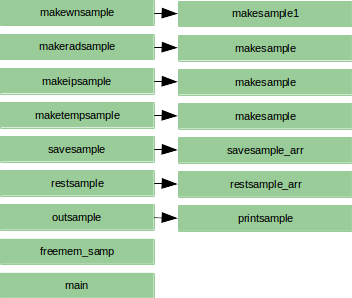
\includegraphics{fig/makesamplec}
\caption{Function structure of makesample.c. The boxes contain function names, and arrows point from a function to the function it calls. Functions are called from left to right, then top to bottom.  Boxes are color-coded as follows:  purple functions are used for eclipse geometry, blue functions are used for transit geometry, green functions are used in both, and red functions are unused at this time.}
\label{fig:makesamplec}
\end{figure}

\subsubsection{List of Functions Defined in makesample.c:}
\function{
int makesample1(prop\_samp *samp, prop\_samp *ref, const long fl)}
\tgray{Create a sampling array. Take values from a reference sampling.} \newline

\function{
int makesample(prop\_samp *samp, prop\_samp *hint, prop\_samp *ref, const long fl)}
\tgray{Create a sampling array. Take values from hint or else from a 
   reference sampling.} \newline

\function{
int makewnsample(struct transit *tr)}
\tgray{Call makesample to create the wavenumber sampling using the
inverse-wavelength values as reference.} \newline

\function{
int makeradsample(struct transit *tr)}
\tgray{Call makesample to create the radius sampling.} \newline

\function{
int makeipsample(struct transit *tr)}
Call makesample to create the impact parameter sampling using the
reversed radius limits and spacing as reference (always produce an
equispaced sampling). \newline

\function{
int maketempsample(struct transit *tr)}
\tgray{Call makesample to create the temperature sampling.} \newline

\function{
static void printsample(FILE *out, prop\_samp *samp, char *desc, long fl)}
Print a sampling's information to file. \newline

\function{
void savesample(FILE *out, prop\_samp *samp)}
Save in binary the sample structure. \newline

\function{
void savesample\_arr(FILE *out, prop\_samp *samp)}
Saves in binary the sample structure's arrays. \newline

\function{
int restsample(FILE *in, prop\_samp *samp)}
Restore a binary sample structure. \newline

\function{
int restsample\_arr(FILE *in, prop\_samp *samp)}
Restore a binary sample structure. \newline

\function{
int outsample(struct transit *tr)}
Print the sample data to file. \newline

\function{
void freemem\_samp(prop\_samp *samp)}
Frees the sampling structure. \newline

\function{
int main(int argc, char *argv[])}
De-bugging. \newline

\subsubsection{makesample1:}
\paragraph{Walkthrough}
\begin{enumerate}[leftmargin=10pt, noitemsep, parsep=0pt, topsep=0ex]
\item[-] Set the acceptable ratio that the final value must fall in to not be truncated.
\item[-] Get sampling units factor, initial value, and final value from the given reference sampling.
\item[-] Raise an error and return -3 if the final value is less than the initial value.
\item[-] Raise an error and return -5 if the reference sampling has no spacing.
\item[-] If the reference sampling has spacing, set the sampling spacing equal to the reference spacing.
\item[-] If the spacing is negative, switch the sign on the acceptable ratio.
\item[-] Set the number of points for the sampling.
\item[-] Ensure that the number of points is positive.
\item[-] Check that the reference sampling has a valid oversampling factor (positive). If not, raise an error and return -6.
\item[-] Set the oversampling factor from the reference oversampling factor.
\item[-] Calculate the number of oversampled points and the spacing between oversampled points.
\item[-] Allocate and fill in sampling values.
\item[-] Check that the final sampling point coincides with the final value. If not, raise a warning.
\item[-] Return 0 (res is 0 for all cases) on success.
\end{enumerate}

\subsubsection{makesample:}
\paragraph{Walkthrough}
\begin{enumerate}[leftmargin=10pt, noitemsep, parsep=0pt, topsep=0ex]
\item[-] Set the acceptable ratio that the final value must fall in to not be truncated.
\item[-] Get sampling units factor from the reference sampling if the hinted sampling is unset or invalid. Otherwise, use the hinted sampling.
\item[-] Get inital and final sampling values from hinted sampling. If hinted sampling is unset or invalid, get them from the reference sampling and update a flag to make note of this.
\item[-] Raise an error and return -5 if the reference sampling has no spacing.
\item[-] If the reference sampling has spacing:
\begin{enumerate}[leftmargin=10pt, noitemsep, parsep=0pt, topsep=0ex]
\item[-] Set the sampling spacing equal to the reference spacing.
\end{enumerate}
\item[-] If the reference sampling does not have spacing:
\begin{enumerate}[leftmargin=10pt, noitemsep, parsep=0pt, topsep=0ex]
\item[-] If the initial and/or final values were taken from the reference sampling rather than the hinted sampling, raise a warning that this happened and that the initial or final values may have been modified.
\item[-] Set the number of samples from the reference sampling.
\item[-] Set the sampling spacing to 0.
\item[-] Allocate sampling values, and copy from reference sampling values.
\item[-] If an oversampling factor was given, raise a warning that this factor will be ignored.
\item[-] Set oversampling factor to 0.
\item[-] Return a flag indicating whether the reference inital and final values were used or not.
\end{enumerate}
\item[-] If a spacing was hinted:
\begin{enumerate}[leftmargin=10pt, noitemsep, parsep=0pt, topsep=0ex]
\item[]- Set sampling spacing to hinted spacing.
\end{enumerate}
\item[-] If none of these spacing conditions are true, raise an error that the sampling inputs are invalid.
\item[-] Raise an error and return -3 if the accepted inital and final sampling values create an invalid (zero or negative) interval.
\item[-] If the sampling spacing is negative, switch the sign on the acceptable ratio.
\item[-] Set the number of points for the sampling.
\item[-] Ensure that the number of points is positive.
\item[-] If the hinted oversampling factor is not given or invalid:
\begin{enumerate}[leftmargin=10pt, noitemsep, parsep=0pt, topsep=0ex]
\item[-] If the reference oversampling factor is not given or invalid, raise an error and return -6.
\end{enumerate}
\item[-] If the hinted oversampling factor is valid, set the sampling oversampling factor equal to the hinted oversampling factor.
\item[-] Calculate the number of oversampled points and the oversampled spacing.
\item[-] Allocate and fill in sampling values.
\item[-] Check that the final sampling point coincides with the final value. If not, raise a warning.
\item[-] Return a flag indicating whether the reference initial and final values were used or not.
\end{enumerate}

\subsubsection{makewnsample:}
\paragraph{Variables Modified:}
\begin{enumerate}[leftmargin=10pt, noitemsep, parsep=0pt, topsep=0ex]
\item[-] Call to \ttblue{makesample} from makesample.c to set \ttred{tr.wns} values.
\item[-] Modify \ttred{tr.pi} to account for {\tt TRPI\_MAKEWN}.
\end{enumerate}

\paragraph{Walkthrough}
\begin{enumerate}[leftmargin=10pt, noitemsep, parsep=0pt, topsep=0ex]
\item[-] If the hinted inital wavenumber sampling value is positive:
\begin{enumerate}[leftmargin=10pt, noitemsep, parsep=0pt, topsep=0ex]
\item[-] If the hinted wavenumber sampling factor is negative, raise an error.
\item[-] Set the reference initial wavenumber sampling value from the hinted initial wavenumber sampling value.
\end{enumerate}
\item[-] Otherwise, if the hinted initial wavelength sampling value is positive:
\begin{enumerate}[leftmargin=10pt, noitemsep, parsep=0pt, topsep=0ex]
\item[-] If the hinted wavenumber sampling factor is negative, raise an error.
\item[-] Set the reference initial wavelength sampling value from the hinted initial wavelength sampling value.
\end{enumerate}
\item[-] Otherwise, if no valid inital wavenumber or wavelength were given, raise an error.
\item[-] If the hinted final wavenumber sampling value is positive:
\begin{enumerate}[leftmargin=10pt, noitemsep, parsep=0pt, topsep=0ex]
\item[-] If the hinted wavenumber sampling factor is negative, raise an error.
\item[-] Set the reference final wavenumber sampling value from the hinted final wavenumber sampling value.
\end{enumerate}
\item[-] Otherwise, if the hinted final wavelength sampling value is positive:
\begin{enumerate}[leftmargin=10pt, noitemsep, parsep=0pt, topsep=0ex]
\item[-] If the hinted wavenumber sampling factor is negative, raise an error.
\item[-] Set the reference final wavelength sampling value from the hinted final wavelength sampling value.
\end{enumerate}
\item[-] Otherwise, if no valid final wavenumber or wavelength were given, raise an error.
\item[-] Set reference oversampling factor from hinted oversampling factor.
\item[-] Set reference unit conversion factor (1).
\item[-] Set reference number of samples to 0.
\item[-] Raise an error if no hinted sampling spacing is given.
\item[-] Set reference sampling spacing from hinted sampling spacing.
\item[-] Call \ttblue{makesample1} from makesample.c to make the oversampled wavenumber sampling.
\item[-] Set reference oversampling factor to 1 (no oversampling).
\item[-] Call \ttblue{makesample1} from makesample.c to make the wavenumber sampling.
\item[-] Call \ttblue{divisors} from iomisc.c to calculate the exact divisors of the oversampling factor.
\item[-] Update progress indicator if sampling was successful.
\item[-] Return the result of \ttblue{makesample1}.
\end{enumerate}

\subsubsection{makeradsample:}
This function makes the radius sample.  Take values from hint or else
from the atmospheric file.  Then the temperature, pressure, mean
molecular mass, itostopes' density, abundance, partition function, and
cross section are also resampled are resampled into an using a linear
or spline interpolation, in case the radius array differ from the
atmospheric radius array (i.e., hint given). \newline

\paragraph{Variables Modified:}
\begin{enumerate}[leftmargin=10pt, noitemsep, parsep=0pt, topsep=0ex]
\item[-] Call to makesample to set \ttred{tr.rads} values.
\item[-] Allocate \ttred{tr.ds.mol.molec.d, tr.ds.mol.molec.q,
    tr.ds.iso.isov.z} (isotope's density, abundance, partition function).
\item[-] Set \ttred{tr.ds.atm.tfct, tr.ds.atm.pfct} from {\tt tr.ds.at.atm.tfct, tr.ds.at.atm.pfct} (atmospheric unit factor for temperature and pressure).
\item[-] Allocate \ttred{tr.atm.t, tr.atm.p, tr.atm.mm} (transit's
  atmospheric temperature, pressure, and mean molecular mass).
\item[-] Set \ttred{tr.atm.t, tr.atm.p, tr.atm.mm} interpolating
  {\tt tr.ds.at.atm} values into {\tt tr.rads} sampling.
\item[-] Set \ttred{tr.ds.iso.isov.d, tr.ds.iso.isov.q}
  interpolating {\tt tr.ds.at.isov} values into {\tt tr.rads}
  sampling.
\item[-] Set \ttred{tr.ds.iso.isov.c, tr.ds.iso.isov.z}
  interpolating {\tt tr.ds.at.isov} values into {\tt tr.atm.t} array.
\item[-] Modify \ttred{tr.pi} to account for {\tt TRPI\_MAKERAD}.
\end{enumerate}

\paragraph{Walkthrough:}
\begin{itemize}[leftmargin=10pt, noitemsep, parsep=0pt, topsep=0ex]
\item[-] Set the reference sampling equal to the atmospheric structure sampling.
\item[-] Check that \ttblue{getatm} and \ttblue{readinfo\_tli} have
  been executed.
\item[-] If a radius sample has already been generated, free the needed memory and unset the corresponding flag.
\item[-] Set flag  to define linear or spline interpolation.
\item[-] If there is only one reference sampling (atmospheric sampling) point:
\begin{itemize}[leftmargin=10pt, noitemsep, parsep=0pt, topsep=0ex]
\item[-] Set all radius sampling parameters to those in the atmospheric radius sampling structure. Allocate and set sampling values.
\item[-] Set result flag to 0.
\end{itemize}
\item[-] Otherwise, if no hinted radius sampling spacing is given:
\begin{itemize}[leftmargin=10pt, noitemsep, parsep=0pt, topsep=0ex]
\item[-] Set all radius sampling parameters to those in the atmospheric radius sampling structure. Allocate and set sampling values.
\item[-] Set result flag to 0.
\end{itemize}
\item[-] Otherwise call \ttblue{makesample} from makesample.c to make the radius sampling.
\item[-] Allocate arrays for molecular density and abundance, and set the number of layers for each molecule.
\item[-] Allocate array for partition function and set the number of layers for each isotope.
\item[-] Allocate arrays for atmospheric temperature, pressure, and mean molecular mass.
\item[-] Call \ttblue{resamplex} from sampling.c to interpolate the radius sampling.
\item[-] Call \ttblue{resampley} from sampling.c to interpolate the atmospheric pressure, temperature, and mean molecular mass.
\item[-] Call \ttblue{resample\_free} from sampling.c to free the resampling arrays.
\item[-] Loop over each database (species):
\begin{itemize}[leftmargin=10pt, noitemsep, parsep=0pt, topsep=0ex]
\item[-] Call \ttblue{resamplex} from sampling.c to interpolate temperatures from the TLI file.
\item[-] Loop over each isotope:
\begin{itemize}[leftmargin=10pt, noitemsep, parsep=0pt, topsep=0ex]
\item[-] Call \ttblue{resampley} from sampling.c to interpolate the partition function from the TLI file.
\end{itemize}
\end{itemize}
\item[-] Call \ttblue{resample\_free} from sampling.c to free the resampling arrays.
\item[-] If sampling was successful, update the progress indicator.
\item[-] Return the result flag.
\end{itemize}


\subsubsection{makeipsample:}
This function makes the impact parameter sampling that determines the
radii at which the planet probed for the transit geometry.  Must be a
decreasing array. If there is no hinted values, it uses the reversed
radius array.
\paragraph{Variables Modified:}
\begin{enumerate}[leftmargin=10pt, noitemsep, parsep=0pt, topsep=0ex]
\item[-] Call to \ttblue{makesample} from makesample.c to set \ttred{tr.ips} values.
\item[-] Modify \ttred{tr.pi} to account for {\tt TRPI\_MAKEIP}.
\end{enumerate}

\paragraph{Walkthrough:}
\begin{itemize}[leftmargin=10pt, noitemsep, parsep=0pt, topsep=0ex]
\item[-] If the hinted radius sampling spacing is -1:
\begin{itemize}[leftmargin=10pt, noitemsep, parsep=0pt, topsep=0ex]
\item[-] Set impact parameter sampling from radius sampling, but reverse the values array.
\end{itemize}
\item[-] Otherwise:
\begin{itemize}[leftmargin=10pt, noitemsep, parsep=0pt, topsep=0ex]
\item[-] Create impact parameter sampling from the hinted sampling parameters.
\item[-] Create reference impact parameter sampling from the radius sampling.
\item[-] Raise an error if the hinted final sampling value is less than the initial sampling value.
\item[-] Check that \ttblue{makeipsample, makeradsample} have been called.
\item[-] Call \ttblue{makesample} from makesample.c to create the impact parameter sampling.
\end{itemize}
\item[-] If desired, call \ttblue{outsample} from makesample.c to print sample information to a file.
\item[-] Update the progress indicator if sampling was successful.
\item[-] Return the result flag.
\end{itemize}


\subsubsection{maketempsample:}
\paragraph{Variables Modified}
\begin{itemize}[leftmargin=10pt, noitemsep, parsep=0pt, topsep=0ex]
\item[-] Call to \ttblue{makesample} from makesample.c to set \ttred{tr.temps} values.
\item[-] Update \ttred{tr.pi} to account for {\tt TRPI\_MAKEIP}.
\end{itemize}

\paragraph{Walkthrough}
\begin{itemize}[leftmargin=10pt, noitemsep, parsep=0pt, topsep=0ex]
\item[-] Create temperature sampling from hinted sampling parameters.
\item[-] Create an empty reference temperature sample.
\item[-] Raise an error if the final sampling value is less than the initial sampling value.
\item[-] Call \ttblue{makesample} from makesample.c to create the temperature sampling.
\item[-] Update the progress indicator if sampling was successful.
\item[-] Return the result flag.
\end{itemize}

\subsubsection{outsample:}
\paragraph{Walkthrough}
\begin{itemize}[leftmargin=10pt, noitemsep, parsep=0pt, topsep=0ex]
\item[-] Check that a filename exists. If not, return 0.
\item[-] If the filename is default and cannot be opened, raise a warning and return 1.
\item[-] Call \ttblue{printsample} from makesample.c to print the following sampling structures:  wavenumber, wavelength, radius, and impact parameter.
\item[-] Close the file.
\item[-] Return 0 on success.
\end{itemize}

\subsubsection{printsample:}
\paragraph{Walkthrough}
\begin{itemize}[leftmargin=10pt, noitemsep, parsep=0pt, topsep=0ex]
\item[-] Print file header.
\item[-] Print sampling factor, inital value, final value, and spacing to file.
\item[-] Print oversampling to file if necessary.
\item[-] Print number of array elements to file.
\item[-] Print sampling values array to file.
\end{itemize}

\newpage
\subsection{opacity.c:}
This file contains routines which calculate opacities, read opacity files, and write opacity files. Figure \ref{fig:opacityc} shows the function structure.

\begin{figure}
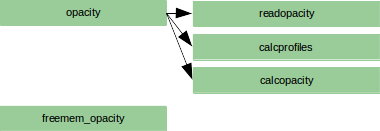
\includegraphics{fig/opacityc}
\caption{Function structure of opacity.c. The boxes contain function names, and arrows point from a function to the function it calls. Functions are called from left to right, then top to bottom.  Boxes are color-coded as follows:  purple functions are used for eclipse geometry, blue functions are used for transit geometry, green functions are used in both, and red functions are unused at this time.}
\label{fig:opacityc}
\end{figure}

\subsubsection{List of Functions Defined in opacity.c:}
\function{
int opacity(struct transit *tr)}
Driver routine to calculate or read the opacity. \newline

\function{
int calcprofiles(struct transit *tr)}
Calculate a grid of Voigt profiles. \newline

\function{
int calcopacity(struct transit *tr, FILE *fp)}
Calculate a grid of opacities and Voigt profiles. \newline

\function{
int readopacity(struct transit *tr, FILE *fp)}
Read an opacity grid from file. \newline

\function{
int extinction(struct transit *tr, int r, int t)}
Calculate the opacity spectrum at a specific layer. \newline

\function{
int freemem\_opacity(struct opacity *op, long *pi)}
Free index of refraction array. \newline

\subsubsection{opacity:}
\paragraph{Modified}
\begin{enumerate}[leftmargin=10pt, noitemsep, parsep=0pt, topsep=0ex]
\item[-] Copy {\tt th.f\_opa} into \ttred{tr.f\_opa}
\end{enumerate}

\paragraph{Walkthrough}
\begin{enumerate}[leftmargin=10pt, noitemsep, parsep=0pt, topsep=0ex]
\item[-] Check that the radius array has been sampled.
\item[-] Check if an opacity file was specified.
\item[-] Call \ttblue{fileexistopen} to check if an opacity file exists and if so, open it.
\item[-] Set the opacity file name in the transit structure from the hint structure.
\item[-] Call \ttblue{readopacity} to read the opacity file if it exists.
\item[-] If the opacity file does not exist:
\begin{enumerate}[leftmargin=10pt, noitemsep, parsep=0pt, topsep=0ex]
\item[-] Open a file for writing.
\item[-] Call \ttblue{calcopacity} from opacity.c to calculate Voigt profiles and the opacity grid if requested.
\end{enumerate}
\item[-] Update the progress indicator to account for {\tt TRPI\_OPACITY}.
\item[-] Return 0 on success.
\end{enumerate}

\subsubsection{calcprofiles:}
\paragraph{Modified}
\begin{enumerate}[leftmargin=10pt, noitemsep, parsep=0pt, topsep=0ex]
\item[-] Copy {\tt tr.ds.th.nDop, tr.ds.th.nLor} into \ttred{tr.ds.op.nDop, tr.ds.op.nLor}.
\item[-] Allocate and set \ttred{tr.ds.op.aDop, tr.ds.op.aLor} equal to logspaces from given minimum and maximum ({\tt tr.ds.th.dmin, tr.ds.th.dmax, tr.ds.th.lmin, tr.ds.th.lmax}).
\item[-] Allocate \ttred{tr.ds.op.profsize} (Voigt profile half-size).
\item[-] Allocate \ttred{tr.ds.op.profile} (Voigt profiles).
\item[-] Call \ttblue{getprofile} from extinction.c to fill out \ttred{tr.ds.op.profsize, tr.ds.op.profile}.
\end{enumerate}

\paragraph{Walkthrough}
\begin{enumerate}[leftmargin=10pt, noitemsep, parsep=0pt, topsep=0ex]
\item[-] Make a logscale grid for the profile widths according to given min and max values.
\item[-] Allocate an array for the profile half-size.
\item[-] Allocate grid of Voigt profiles.
\item[-] Loop over all Doppler and Lorentz widths to calculate Voigt profiles
\begin{enumerate}[leftmargin=10pt, noitemsep, parsep=0pt, topsep=0ex]
\item[-] If the Doppler width is an order of magnitude smaller than the Lorentz width, and this is not the first calculation performed, set the profile half-size equal to the previous profile(skipping the calculation)
\item[-] Otherwise, call to \ttblue{getprofile} in extinction.c to calculate Voigt profile half-size.
\end{enumerate}
\item[-] Return 0 on success.
\end{enumerate}

\subsubsection{calcopacity:}
\paragraph{Modified}
\begin{enumerate}[leftmargin=10pt, noitemsep, parsep=0pt, topsep=0ex]
\item[-] Copy {\tt tr.temp.n} into \ttred{tr.ds.op.Ntemp}.
\item[-] Allocate \ttred{tr.ds.op.temp} (temperature array) and copy from {\tt tr.temp.v}.
\item[-] Allocate and evaluate \ttred{tr.ds.op.ziso} (Partition function for each isotope and temperature).
\item[-] Copy {\tt tr.rads.n} into \ttred{tr.ds.op.Nlayer} (number of radius layers).
\item[-] Allocate \ttred{tr.ds.op.press} (pressure array) and copy from {\tt tr.atm.p} in CGS units.
\item[-] Copy {\tt tr.ds.iso.nmol} into \ttred{tr.ds.op.Nmol} (number of molecules).
\item[-] Allocate \ttred{tr.ds.op.molID} (molecule IDs).
\item[-] Add molecule IDs to \ttred{tr.ds.op.molID} if not there.
\item[-] Copy {\tt tr.wns.n} into \ttred{tr.ds.op.Nwave} (number of wavenumber samples).
\item[-] Allocate \ttred{tr.ds.op.wns} and copy from {\tt tr.wns.v} (wavenumber samples).
\item[-] Allocate \ttred{tr.ds.op.o} (4D opacity array).
\end{enumerate}

\paragraph{Walkthrough}
\begin{enumerate}[leftmargin=10pt, noitemsep, parsep=0pt, topsep=0ex]
\item[-] Call \ttblue{maketempsample} from makesample.c to create a temperature array from hinted values and put the temperature array in the opacity structure.
\item[-] Allocate the partition function array.
\item[-] Set the interpolation function flag.
\item[-] Interpolate the isotope partition function for each isotope in each database.
\item[-] Get pressure array from the transit structure and place in the opacity structure.
\item[-] Get molecule array from the transit structure and place in the opacity structure.
\item[-] For each molecule, check if its ID is in the molecule ID array. If not, add it.
\item[-] Get wavenumber array from the transit structure and place in the opacity structure.
\item[-] Allocate the 4-dimensional opacity array ([mol][temp][rad][wn])
\item[-] For each radius layer and temperature, call to \ttblue{extinction} in opacity.c to compute extinction.
\item[-] Write dimension sizes to file.
\item[-] Write molecular ID, temperature, pressure, and wavenumber sampling arrays to file.
\item[-] Write the opacity array to file.
\item[-] Close the file.
\item[-] Return 0 on success.
\end{enumerate}

\subsubsection{readopacity:}
\paragraph{Modified}
\begin{enumerate}[leftmargin=10pt, noitemsep, parsep=0pt, topsep=0ex]
\item[-] Allocate \ttred{tr.ds.op.molID, tr.ds.op.temp, tr.ds.op.press, tr.ds.op.wns} and fill in from file.
\item[-] Allocate \ttred{tr.ds.op.o} and fill in from file.
\end{enumerate}

\paragraph{Walkthrough}
\begin{enumerate}[leftmargin=10pt, noitemsep, parsep=0pt, topsep=0ex]
\item[-] Read the dimension sizes (number of molecules, temperatures, radius layers, and wavenumbers) from file.
\item[-] Allocate molecular ID, temperature, pressure, and wavenumber sampling arrays.
\item[-] Read molecular ID, temperature, pressure, and wavenumber sampling arrays from file.
\item[-] Allocate the 4D opacity grid.
\item[-] Read the opacity grid from file.
\item[-] Return 0 on success.
\end{enumerate}

\newpage
\subsection{crosssec.c:}
This file contains routines which are used to read the cross-section (CS) files(s) and interpolate the values therein to the {\tt transit} sampling. Figure \ref{fig:crosssec} shows the function structure of crosssec.c.

\begin{figure}
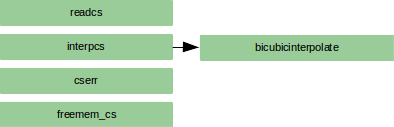
\includegraphics{fig/crosssec}
\caption{Function structure of crosssec.c. The boxes contain function names, and arrows point from a function to the function it calls. Functions are called from left to right, then top to bottom.  Boxes are color-coded as follows:  purple functions are used for eclipse geometry, blue functions are used for transit geometry, and green functions are used in both.}
\label{fig:crosssec}
\end{figure}

\subsubsection{List of Functions Defined in crosssec.c:}
\function{
int readcs(struct transit *tr)}
Read cross-section (CS) info from tabulated files. \newline

\function{
int interpolatecs(struct transit *tr)}
\tgray{Get number of CS files from hint. Allocate tr.ds.cia variables.
Open files, read isotope names and sampled temperatures.
Read tabulated data (wavenumber x temperatures).
Interpolate values from tabulated sample to transit sample.
Get density arrays of the isotopes from transit.
Calculate absorption coefficients in cm$\sp{-1}$.} \newline

\function{
int bicubicinterpolate(&double **res, double **src, double *x1, long nx1, 
                    \\ &double *x2, long nx2, double *t1, long nt1, 
                    \\ &double *t2, long nt2)}
\tgray{Interpolates 'src' into 'res' according to the new dimensions, first
interpolates the second dimension and then the first. The result is
added to 'res'.} \newline

\function{
void cserr(int max, char *name, int line)}
\tgray{Error printing function for lines longer than maxline in the CS file.} \newline

\function{
int freemem\_cs(struct cross *cross, long *pi)}
\tgray{Free cross-section structure.} \newline

\subsubsection{readcs:}
\paragraph{Modified}
\begin{enumerate}[leftmargin=10pt, noitemsep, parsep=0pt, topsep=0ex]
\item[-] Allocate \ttred{tr.ds.cross.e} (CS extinction array).
\item[-] Allocate \ttred{tr.ds.cross.mol1, tr.ds.cross.mol2} (molecule IDs).
\item[-] Allocate \ttred{tr.ds.cross.ntemp, tr.ds.cross.nwave} (number of temperatures per file, number of wavenumbers per file).
\item[-] Allocate \ttred{tr.ds.cross.cs, tr.ds.cross.temp, tr.ds.cross.wn, tr.ds.cross.nspec} (3D CS array, temperature array, wavenumber array, number of species per file).
\item[-] Copy {\tt tr.ds.th.nfiles} into \ttred{tr.ds.cross.nfiles}.
\item[-] Fill in \ttred{tr.ds.cross.cs, tr.ds.cross.wn, tr.ds.cross.temp, tr.ds.cross.ntemp, \\ tr.ds.cross.nwave, tr.ds.cross.mol1, tr.ds.cross.mol2} from file.
\item[-] Update \ttred{tr.pi} to account for {\tt TRPI\_CS}.
\end{enumerate}

\paragraph{Walkthrough}
\begin{enumerate}[leftmargin=10pt, noitemsep, parsep=0pt, topsep=0ex]
\item[-] Check that radius and wavenumber samples have been made.
\item[-] Allocate extinction array in cross-section structure.
\item[-] If there are no CS files, return 0.
\item[-] Allocate molecule names, molecule IDs, number of molecules in each file, number of temperatures and wavenumber samples per file, and CS array.
\item[-] Loop over each CS file:
\begin{enumerate}[leftmargin=10pt, noitemsep, parsep=0pt, topsep=0ex]
\item[-] Read the file name from the transit hint structure.
\item[-] Open the file.
\item[-] Skip any comments and blank lines at the top of the file.
\item[-] When an 'i' character is encountered:
\begin{enumerate}[leftmargin=10pt, noitemsep, parsep=0pt, topsep=0ex]
\item[-] If pointing to a blank space, increment the pointer to the next character.
\item[-] Count the number of words in the line. If not 1 or 2, raise an error.
\item[-] Loop over each molecule, copy the name of the molecule and find its ID by comparing its name with the molecule IDs. Raise an error if the molecule from file does not match any IDs.
\item[-] Continue reading the file.
\end{enumerate}
\item[-] When a 't' character is encountered:
\begin{enumerate}[leftmargin=10pt, noitemsep, parsep=0pt, topsep=0ex]
\item[-] If pointing to a blank space, increment the pointer to the next character.
\item[-] Count the number of temperature samples in the file.
\item[-] Raise an error if no temperature samples are found.
\item[-] Loop over the temperatures and copy them into the cross-section temperature array.
\item[-] Continue reading the file.
\end{enumerate}
\item[-] Set the initial value for allocated wavenumber fields.
\item[-] Allocate the wavenumber and extinction arrays.
\item[-] Begin infinite loop to read in data:
\begin{enumerate}[leftmargin=10pt, noitemsep, parsep=0pt, topsep=0ex]
\item[-] Increment the pointer past all comments and blank lines.
\item[-] Check if the end of the file has been reached. If so, break the loop.
\item[-] Check if the number of read wavelengths is equal to the allocated wavenumber fields. If so, reallocate the array to double its size by bitwise left-shifting the number of fields. A bitwise left-shift doubles the value.
\item[-] Increment the pointer past all blank spaces
\item[-] Read in the wavenumber at pointer location.
\item[-] Loop over each temperature and copy the corresponding extinction value to the extinction array.
\item[-] Increment looping indices.
\end{enumerate}
\item[-] Reallocate the arrays to remove extra rows added when doubling the size.
\item[-] Store the extinction array in the cross-section structure.
\item[-] Close the file.
\end{enumerate}
\item[-] Update the progress indicator to account for {\tt TRPI\_CS}.
\item[-] Return 0 on success.
\end{enumerate}

\subsubsection{interpcs:}
\paragraph{Modified}
\begin{enumerate}[leftmargin=10pt, noitemsep, parsep=0pt, topsep=0ex]
\item[-] Fill out \ttred{tr.ds.cross.e} by calling \ttblue{bicubicinterpolate} for each cross-section file.
\end{enumerate}

\paragraph{Walkthrough}
\begin{enumerate}[leftmargin=10pt, noitemsep, parsep=0pt, topsep=0ex]
\item[-] Allocate temporary temperature and wavenumber arrays.
\item[-] Reset cross-section opacity to zero.
\item[-] Allocate temporary array for opacity.
\item[-] Set tempoarary temperature and wavenumber arrays from the transit structure.
\item[-] For each cross-section file:
\begin{enumerate}[leftmargin=10pt, noitemsep, parsep=0pt, topsep=0ex]
\item[-] Call \ttblue{bicubicinterpolate} from crosssec.c to interpolate CS data to the wavenumber and temperature sampling.
\item[-] Get density profiles of isotopes from molecular information structure.
\item[-] Calculate cross-section absorption coefficients at each radius and wavenumber.
\end{enumerate}
\item[-] Free temporary arrays.
\item[-] Return 0 on success. 
\end{enumerate}

\subsubsection{bicubicinterpolate:}
\paragraph{Walkthrough}
\begin{enumerate}[leftmargin=10pt, noitemsep, parsep=0pt, topsep=0ex]
\item[-] Set the first and last values of the source array.
\item[-] Check that the sampling regions match. If not, return 0.
\item[-] Find indices where the target array is within the source array boundaries (so that the result is an interpolation, not an extrapolation).
\item[-] Call \ttblue{splinterp\_pt} from spline.c to perform cubic interpolation over the first index.
\item[-] Call \ttblue{splinterp\_pt} from spline.c to perform cubic interpolation over the second index.
\item[-] Free temporary arrays.
\item[-] Return 0.
\end{enumerate}

\newpage
\subsection{idxrefraction.c:}
This file is concerned with calculating the index of refraction at each radius level. Currently this is 1 at all layers (no light bending). Functions \ttblue{restidxref, saveidxref} are unused. Figure \ref{fig:idxrefracc} shows the function structure of idxrefraction.c

\begin{figure}
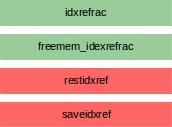
\includegraphics{fig/idxrefractionc}
\caption{Function structure of idxrefrac.c. The boxes contain function names, and arrows point from a function to the function it calls. Functions are called from left to right, then top to bottom.  Boxes are color-coded as follows:  purple functions are used for eclipse geometry, blue functions are used for transit geometry, green functions are used in both, and red functions are unused at this time.}
\label{fig:idxrefractionc}
\end{figure}

\subsubsection{List of Functions Defined in idxrefraction.c:}
\function{
int idxrefrac(struct transit *tr)}
\tgray{Calculates the index of refraction.  Currently, it sets an index of
refraction of 1.0 at all levels (no light bending).} \newline

\function{
int freemem\_idexrefrac(struct idxref *ir, long *pi)}
\tgray{Free index of refraction array.} \newline

\function{
int restidxref(FILE *in, PREC\_NREC nrad, struct idxref *ir)}
\tgray{Restore hints structure, the structure needs to have been
allocated before.} \newline

\function{
void saveidxref(FILE *out, PREC\_NREC nrad, struct idxref *ir)}
\tgray{Write index of refraction values to file pointed by out.} \newline

\subsubsection{idxrefrac:}
\paragraph{Variables Modified}
\begin{enumerate}[leftmargin=10pt, noitemsep, parsep=0pt, topsep=0ex]
\item[-] Allocate and set values of \ttred{tr.ds.ir.n} (Index of
  refraction per radius array)
\item[-] Update \ttred{tr.pi} to account for {\tt TRPI\_IDXREFRAC}.
\end{enumerate}

\paragraph{Walkthrough}
\begin{enumerate}[leftmargin=10pt, noitemsep, parsep=0pt, topsep=0ex]
\item[-] Call to \ttblue{transitcheckcalled} in transitstd.c to check that \ttblue{makeradsample} has been called.
\item[-] Allocate index of refraction array.
\item[-] Loop over each radius layer:
\begin{enumerate}[leftmargin=10pt, noitemsep, parsep=0pt, topsep=0ex]
\item[-] Call to \ttblue{stateeqnford} from transit.h to calculate density.
\item[-] Calculate index of refraction (currently always 1).
\end{enumerate}
\item[-] Return 0 on success.
\end{enumerate}

\newpage
\subsection{extinction.c:}
This file contains routines associated with computing molecular extinction. That includes a wrapper function to calculate Voigt profiles, a function to compute molecular extinction, and a function to interpolate the molecular extinction. There are also functions which compute extinction from other sources (\ttblue{computeextscat, computeextcloud}) although they are not fully implemented. Functions \ttblue{savefile\_extinct, restfile\_extinct, restextinct} are unused. Figure \ref{fig:extinctionc} shows the function structure of extinction.c.

\begin{figure}
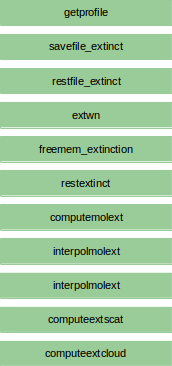
\includegraphics{fig/extinctionc}
\caption{Function structure of extinction.c. The boxes contain function names, and arrows point from a function to the function it calls. Functions are called from left to right, then top to bottom.  Boxes are color-coded as follows:  purple functions are used for eclipse geometry, blue functions are used for transit geometry, green functions are used in both, and red functions are unused at this time.}
\label{fig:extinctionc}
\end{figure}

\subsubsection{ List of Functions Defined in extinction.c:}
\function{
inline int getprofile(&PREC\_VOIGT **pr, int vf, PREC\_RES dwn, PREC\_VOIGT dop,
                   \\ & PREC\_VOIGT lor, float ta)}
\tgray{Driver to calculate a Voigt profile.} \\

\function{
void savefile\_extinct(&char *filename, PREC\_RES **e, \_Bool *c, long nrad, 
                    \\ &long nwav)}
\tgray{Saving extinction for a possible next run} \newline

\function{
void restfile\_extinct(&char *filename, PREC\_RES **e, \_Bool *c, long nrad,
                    \\ &long nwav)}
\tgray{Restoring extinction for a possible next run} \\

\function{
int extwn(struct transit *tr)}
\tgray{Fill up the extinction information} \\

\function{
void printone(struct transit *tr)}
\tgray{Printout for one P,T conditions} \\

\function{
int freemem\_extinction(struct extinction *ex, long *pi)}
\tgray{Free extinction coefficient structure arrays} \\

\function{
int restextinct(&FILE *in, PREC\_NREC nrad, short niso, PREC\_NREC nwn, 
             \\ &struct extinction *ex)}
\tgray{Restore hints structure, the structure needs to have been allocated before} \\

\function{
int computemolext(struct transit *tr, PREC\_NREC r, PREC\_RES **kiso)}
\tgray{Compute the molecular extinction.} \\

\function{
int interpolmolext(struct transit *tr, PREC\_NREC r, PREC\_RES **kiso)}
\tgray{Interpolate the opacity grid at the specified layer to obtain
  molecular extinction.}  \\

\function{
void computeextscat(double *e, long n, struct extscat *sc, double *rad, \\
                    double trad, double *temp, double tcft, double wn)}
\tgray{Compute scattering contribution to extinction. Currently fills the scattering extinction array with 0's (no extinction due to scattering).} \\

\function{
void computeextcloud(double *e, long n, struct extscat *sc, double *rad, \\
                     double trad, double *temp, double tcft, double wn)}
\tgray{Compute cloud contribution to extinction. Cloud extinction is linear, increasing from top of the clouds to the bottom of the clouds.} \\

\subsubsection{getprofile}
\paragraph{Variables Modified}
\begin{enumerate}[leftmargin=10pt, noitemsep, parsep=0pt, topsep=0ex]
\item[-] Allocate \ttred{op.profile} (**pr).
\end{enumerate}

\paragraph{Walkthrough}
\begin{enumerate}[leftmargin=10pt, noitemsep, parsep=0pt, topsep=0ex]
\item[-] Find the largest width between Doppler and Lorentz
\item[-] Calculate the range for computation in half-widths.
\item[-] Calculate the number of points in the profile.
\item[-] Check that the profile contains at least 3 elements. If not, set to 3.
\item[-] If the profile is larger than the wavenumber range, shrink the profile.
\item[-] Allocate the profile array.
\item[-] Calculate the Voigt profile using a width that gives and integer number of {\tt dwn} spaced bins. See Equations \ref{eqn:doppler}, \ref{eqn:lorentz}.
\item[-] Return the number of points in half the profile.
\end{enumerate}

\subsubsection{extwn:}
\paragraph{Modified:}
\begin{enumerate}[leftmargin=10pt, noitemsep, parsep=0pt, topsep=0ex]
\item[-] Copy {\tt tr.ds.th.ethresh} into \ttred{tr.ds.ex.ethresh} (extinction threshold).
\item[-] Allocate \ttred{tr.ds.ex.e} (extinction).
\item[-] Allocate \ttred{tr.ds.ex.computed} (boolean to indicate if extinction has been computed at the corresponding radius layer).
\item[-] Update \ttred{tr.pi} to account for {\tt TRPI\_EXTWN}.
\end{enumerate}

\paragraph{Walkthrough:}
\begin{enumerate}[leftmargin=10pt, noitemsep, parsep=0pt, topsep=0ex]
\item[-] Check that \ttblue{readinfo\_tli, readdatarng, makewnsample,
    makeradsample} have been executed.
\item[-] Set extinction coefficient threshold from transithint structure.
\item[-] Allocate extinction coefficient array.
\item[-] Allocate boolean for checing if extinction has been computed.
\item[-] Update progress indicator to account for {\tt TRPI\_EXTWN}.
\end{enumerate}

\subsubsection{computemolext:}
This routine computes the molecular extinction coefficient ($e_m$, in
cm$^{-1}$) at one specific atmospheric radius, Equations
(3.36)--(3.37) of P. Rojo's thesis (see also Equation
\ref{eqn:ext}).  Initially, the code calculates the Doppler and
Lorentz line-broadening widths (Equations \ref{eqn:doppler} and
\ref{eqn:lorentz}), to later calculate the Voigt profile.

\paragraph{Modified}
\begin{enumerate}[leftmargin=10pt, noitemsep, parsep=0pt, topsep=0ex]
\item[-] Calculate \ttred{tr.ds.ex.e} (Extinction coefficient) for the given radius layer.
\item[-] Set \ttred{tr.ds.ex.computed} of given radius to True.
\end{enumerate}

\paragraph{Walkthrough}
\begin{enumerate}[leftmargin=10pt, noitemsep, parsep=0pt, topsep=0ex]
\item[-] Allocate alpha Lorentz and Doppler arrays.
\item[-] Allocate Lorentz and Doppler width indices arrays
\item[-] Allocate arrays for max and min extinction for each species.
\item[-] Allocate a temporary extinction array.
\item[-] Calculate the dynamic wavenumber sampling interval and the oversampled dynamic wavenumber sampling interval.
\item[-] Calculate constant factors for Doppler and Lorentz line widths.
\item[-] Allocate arrays for the Doppler and Lorentz line widths and arrays for line width indices.
\item[-] Loop over each isotope.
\begin{enumerate}[leftmargin=10pt, noitemsep, parsep=0pt, topsep=0ex]
\item[-] Loop over each molecular species.
\begin{enumerate}[leftmargin=10pt, noitemsep, parsep=0pt, topsep=0ex]
\item[-] Calculate the isotope's collisional cross-section with this molecule and add the resulting Lorentz width to the Lorentz width for this isotope.
\end{enumerate}
\item[-] Multiply by the constant factor to get the Lorentz width for this isotope.
\item[-] Calculate the Doppler width divided by the central wavenumber (because Doppler width is wavenumber-dependent).
\item[-] Find the maximum between the Lorentz width and Doppler width.
\item[-] Find the minimum between this maximum and the previously calculated minimum (this minimum is set to the maximum between the widths on the first iteration).
\item[-] Call \ttblue{binsearchapprox} from iomisc.c to perform a binary search to find the indices of the Doppler and Lorentz widths in the Doppler and Lorentz width samples.
\end{enumerate}
\item[-] Set oversampling resolution by looping through the exact divisors of the oversampling factor until the divisor times the spacing of the finest oversampling is greater than half the width of the smallest profile.
\item[-] Loop over every line to calculate the maximum extinction coefficient for each molecule.
\begin{enumerate}[leftmargin=10pt, noitemsep, parsep=0pt, topsep=0ex]
\item[-] Calculate the wavenumber of the line transition.
\item[-] Skip calculation for this line transition if it is not within the given limits.
\item[-] Calculate the extinction coefficient except the broadening factor (this is proportional to the extinction).
\item[-] If the maximum extinction for this molecule has not been calculated yet, set it equal to the extinction coefficient that was just calculated. Otherwise, set the maximum and minimum extinction for this molecule equal to the maximum and minimum between the recently calculated extinction and the previously calculated maximum and minimum.
\end{enumerate}
\item[-] Loop over each line to calculate extinction coefficients.
\begin{enumerate}[leftmargin=10pt, noitemsep, parsep=0pt, topsep=0ex]
\item[-] Calculate the wavenumber of the line transition.
\item[-] Skip calculation for this line transition if it is not within the given limits.
\item[-] Calculate the extinction coefficient. (FINDME: reference equation)
\item[-] Find the index of the closest oversampled wavenumber.
\item[-] Check if the next line falls within the same sampling unit (same sampling index). If so, co-add the next line with the current line (add the next line's extinction to the opacity for this line) and skip the next line's calculations.
\item[-] If the extinction for this line is less than the defined threshold factor times the maximum extinction, disregard this line and continue to the next.
\item[-] Calculate the closest dynamic sampling wavenumber.
\item[-] Check if the ratio of Doppler width to Lorentz width is greater than a given threshold. If so, call to \ttblue{binsearchapprox} to do a binary search to recalculate the index for the Doppler width. If not, then the exact width of the Doppler profile is unimportant and the calculation is skipped.
\item[-] Calculate the offset between the center of the line and the dynamic wavenumber sample (in units of oversampled wavenumber spacing).
\item[-] Calculate the offset between the edge of the profile and the beginning of the wavenumber array (in units of oversampled wavenumber spacing).
\item[-] Calculate the lower and upper indices of the profile (in units of dynamically sampled wavenumber)
\item[-] Fix the lower and upper indices to the boundaries if they go outside the bounds of the wavenumber sampling.
\item[-] Add the contribution from this line (and any co-added lines) to the opacity spectrum.
\end{enumerate}
\item[-] Call \ttblue{downsample} to downsample the temporary extinction array to the final sampling size and fill in the extinction array for this radius.
\item[-] Free all temporary arrays.
\item[-] Update the boolean that indicates extinction has been computer for this layer.
\item[-] Return 0 on success.
\end{enumerate}


\subsubsection{interpolmolext:}
\paragraph{Modified}
\begin{enumerate}[leftmargin=10pt, noitemsep, parsep=0pt, topsep=0ex]
\item[-] Fill in \ttred{tr.ds.ex.e}. 
\item[-] Set the radius index of \ttred{tr.ds.ex.computed} equal to 1.
\end{enumerate}

\paragraph{Walkthrough}
\begin{enumerate}[leftmargin=10pt, noitemsep, parsep=0pt, topsep=0ex]
\item[-] Perform a binary search to find the index of grid-temperature immediately lower than layer temperature.
\item[-] Loop over wavenumber
\begin{enumerate}[leftmargin=10pt, noitemsep, parsep=0pt, topsep=0ex]
\item[-] Loop over molecules
\begin{enumerate}[leftmargin=10pt, noitemsep, parsep=0pt, topsep=0ex]
\item[-] Calculate extinction coefficient by linear interpolation of the opacity grid between the index found by the binary search and the next one.
\item[-] Call \ttblue{valueinarray} to find the index of the molecule.
\item[-] Add the extinction for this molecule to extinction
\end{enumerate}
\end{enumerate}
\item[-] Update boolean to show extinction has been computed.
\item[-] Return 0 on success.
\end{enumerate}

\subsubsection{computeextscat:}
\paragraph{Modified}
\begin{enumerate}[leftmargin=10pt, noitemsep, parsep=0pt, topsep=0ex]
\item[-] Fill out scattering extinction array (passed to function, not found in any structures).
\end{enumerate}

\paragraph{Walkthrough}
\begin{enumerate}[leftmargin=10pt, noitemsep, parsep=0pt, topsep=0ex]
\item[-] Loop over each radius layer. Set scattering extinction to 0 at all layers.
\end{enumerate}

\subsubsection{computeextcloud:}
\paragraph{Modified}
\begin{enumerate}[leftmargin=10pt, noitemsep, parsep=0pt, topsep=0ex]
\item[-] Fill out cloud extinction array (passed to function, not found in any structures).
\end{enumerate}

\paragraph{Walkthrough}
\begin{enumerate}[leftmargin=10pt, noitemsep, parsep=0pt, topsep=0ex]
\item[-] If there are no clouds, set the cloud extinction array to zero everywhere.
\item[-] Calculate the amount of extinction per distance due to the clouds.
\item[-] Loop down through the radius layers, setting the cloud extinction to 0 until reaching the clouds.
\item[-] Loop down through the radius layers, starting from the top of the clouds, setting the cloud extinction to a linearly increasing amount according to the extinction per distance until reaching the bottom of the clouds.
\item[-] Loop through the remaining radius layers, setting the cloud extinction to the total extinction due to clouds.
\end{enumerate}

\newpage
\subsection{tau.c:}
This file contains all routines associated with calculation of optical depth. Functions \ttblue{detailout}, \ttblue{outdebtauex}, \ttblue{outdebex}, and \ttblue{outdebtau} are unused. Functions \ttblue{print2dArrayDouble, print1dArrayDouble} are generic print-to-file functions that are not generally used in {\tt transit}. Figure \ref{fig:tauc} shows the function structure of tau.c.
\findme{reference the equation in BART theory doc}

\begin{figure}
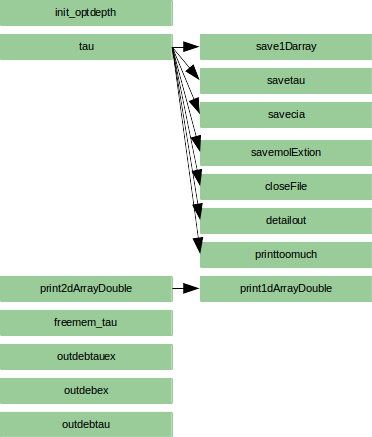
\includegraphics{fig/tauc}
\caption{Function structure of tau.c. The boxes contain function names, and arrows point from a function to the function it calls. Functions are called from left to right, then top to bottom.  Boxes are color-coded as follows:  purple functions are used for eclipse geometry, blue functions are used for transit geometry, green functions are used in both, and red functions are unused at this time.}
\label{fig:tauc}
\end{figure}

\subsubsection{List of Functions Defined in tau.c:}

\function{
int init\_optdepth(struct transit *tr)}
\tgray{Initialize the optical depth structure for eclipse and transit geometry.} \newline

\function{
int tau(struct transit *tr)}
\tgray{Calculate the extinction coefficient and optical depth as a function
of layer/impact parameter and wavelength.} \newline

\function{
int detailout(&prop\_samp *wn, prop\_samp *rad, struct detailfld *det,
           \\ &PREC\_RES **arr, short flag)}
\tgray{Print to file the optical depth, cia, or extinction at the
requested wavenumbers (given by det).} \newline

\function{
void printtoomuch(&char *file, struct optdepth *tau, prop\_samp *wn,
               \\ &prop\_samp *rad)}
\tgray{Print (to file or stdout) the impact parameter where the optical depth
reached toomuch (for each wavenumber).} \newline

\function{
int freemem\_tau(struct optdepth *tau, long *pi)}
\tgray{Free tau structure.} \newline

\function{
void outdebtauex(&char *name, PREC\_RES **e, prop\_samp *ip, PREC\_RES **t,
              \\ &long rn, long w)}
\tgray{Print to file (name) the optical depth and extinction as a function of
impact parameter (up to layer index rn), for given wavenumber (with
index w).} \newline

\function{
void outdebex(&char *name, PREC\_RES **e, PREC\_RES *r, long rn, long wi,
           \\ &long wf)}
\tgray{Print to file (name) the extinction coefficient as a function of radius
   (up to layer index rn) for the specified wavenumber range (indices from
    wi to wf).} \newline

\function{
void outdebtau(char *name, prop\_samp *ip, PREC\_RES **t, long wi, long wf)}
\tgray{Print to file (name) the optical depth as function of impact parameter
   for the specified wavenumber range (indices from wi to wf).} \newline


\subsubsection{tau:}
Main routine where the extinction coefficient and the optical depth
are calculated.  This function sets up the optical depth parameters and
then calls to the \ttblue{computeextradius} and \ttblue{totaltau}
subroutines to do the calculations.

In the code, \ttblue{transittau} or \ttblue{eclipsetau} is pointed by
the variable \ttblue{fcn}. \ttblue{transittau} is defined in the
\texttt{transit\_ray\_solution slantpath} variable at the end of
slantpath.c. \ttblue{eclipsetau} is defined in the 
\texttt{transit\_ray\_solution eclipsepath} variable at the end of
eclipse.c. \texttt{slantpath} is assigned to the transit
variable \ttred{tr.sol} in the function \ttblue{acceptgenhints} from
\texttt{argum.c}.

\paragraph{Variables Modified:}
\begin{enumerate}[leftmargin=10pt, noitemsep, parsep=0pt, topsep=0ex]
\item[-] Copy \ttred{tr.save.ext} from {\tt th.save.ext} (extinction
  output filename).
\item[-] Call to {\tt init\_optdepth} to initialize {\tt tr.tau}.
\item[-] Set \ttred{tr.cl.cloudext, tr.cl.cloudtop, tr.cl.cloudbottom}
  (Cloud maximum opacity, top layer radius, layer radius of cloudext).
\item[-] Call to {\tt computemolext} or {\tt interpolmolext} to calculate
  \ttred{tr.ds.ex.e} (extinction coefficient).
\item[-] Call to {\tt eclipsetau} or {\tt transittau} to calculate
  \ttred{tr.tau.t} (optical depth).
\item[-] Set \ttred{tr.tau.last} if {\tt tr.tau.t > toomuch}
  (radius index of last calculated tau).
\item[-] Call to {\tt savefile\_extinct} to store {\tt tr.ds.ex.e} in
  file.
\item[-] Call to {\tt printtoomuch} to store the radius where the
  optical depth reached toomuch.
\item[-] Call to {\tt freemem\_lineinfotrans} to free
  \ttred{tr.ds.li} (line info struct).
\item[-] Call to {\tt freemem\_localextinction} to free
  \ttred{tr.ds.ex.e} and related static variables (extinction
  coefficient).
\item[-] Update \ttred{tr.pi} to account for {\tt TRPI\_TAU}.
\end{enumerate}

\paragraph{Walkthrough:}
\begin{enumerate}[leftmargin=10pt, noitemsep, parsep=0pt, topsep=0ex]
\item[-] Store the height of each layer (eclipse) or impact parameter (transit)
     starting from the outermost layer in local variable {\tt h}.
\item[-] Check that there are enough radius layers for interpolation (4+).  If not, raise an error.
\item[-] Check that idxrefrac and extwn functions have been called.
\item[-] Pass {\tt TAU} flags from transithint structure to transit structure.
\item[-] Declare arrays for cloud and scattering extinction (per wavenumber).
\item[-] Call to \ttblue{restfile\_extinct} from extinction.c to restore extinction save file (if requested).
\item[-] Compute molecular extinction at the outermost layer.
\item[-] Start loop, over wavenumber, to calculate the extinction:
\begin{enumerate}[leftmargin=10pt, noitemsep, parsep=0pt, topsep=0ex]
  \item[-] Compute the scattering and cloud extinction for all layers at
    given wavenumber.
  \item[-] Start loop, over the layers/impact parameters:
  \begin{enumerate}[leftmargin=10pt, noitemsep, parsep=0pt, topsep=0ex]
  \item[-] Check if the molecular extinction has been calculated at this
    layer. If not, call to \ttblue{interpolmolext} (if an opacity file exists) or \ttblue{computemolext} (if there is no opacity file and there is a TLI file) from extinction.c calculate it for all wavenumbers at this layer.
  \item[-] Call \ttblue{transittau} or \ttblue{eclipsetau} (as fcn) to calculate the
    optical depth at given wavenumber and layer/impact parameter. See Equation \ref{eqn:tau}.
  \item[-] If the optical depth reached toomuch, end the
    layer/impact-parameter loop.
  \end{enumerate}
  \item[-] Call to \ttblue{save1Darray} from tau.c to save total extinction, cloud extinction, and scattering 
    extinction if requested.
\end{enumerate}
\item[-] Call to \ttblue{savetau, saveCIA, savemolExtion} from tau.c to print to file the 2D arrays of tau, extinction, and CIA if requested. Call to \ttblue{closeFile} from iomisc.c to close these files.
\item[-] Call to \ttblue{detailout} from argum.c to print detailed output of optical depth, extinction, and CIA to file if requested.
\item[-] Call to \ttblue{printtoomuch} from tau.c to print to file the lowest layer/impact parameter reached before
  optical depth reached toomuch.
\item[-] Update the progress indicator.
\item[-] Return 0 on success.
\end{enumerate}


\subsubsection{init\_optdepth:}
\paragraph{Variables Modified:}
\begin{enumerate}[leftmargin=10pt, noitemsep, parsep=0pt, topsep=0ex]
\item[-] Initialize \ttred{tr.ds.tau} and \ttred{tr.ds.intens}.
\item[-] Set \ttred{tr.tau.toomuch} from {\tt th.toomuch} (max
  optical depth to calculate).
\item[-] Allocate \ttred{tr.tau.t, tr.tau.last} (optical depth and
  index of toomuch).
\item[-] Allocate \ttred{tr.ds.intens.a} (intensity grid).
\end{enumerate}

\paragraph{Walkthrough:}
\begin{enumerate}[leftmargin=10pt, noitemsep, parsep=0pt, topsep=0ex]
\item[-] Allocate the optical depth structure.
\item[-] Pull maximum optical depth from transithint structure into optical depth structure.
\item[-] Allocate array for the layer index where tau reaches toomuch (max optical depth).
\item[-] Allocate the optical depth array
\item[-] Allocate the intensity grid structure and intensity array if using eclipse geometry.
\item[-] Return 0 on success.
\end{enumerate}

\subsubsection{detailout:}
\paragraph{Walkthrough:}
\begin{enumerate}[leftmargin=10pt, noitemsep, parsep=0pt, topsep=0ex]
\item[-] Check that there a file name has been given.
\item[-] Perform a binary search to find the indices of the requested wavenumbers.
\item[-] Print wavenumber.
\item[-] Print radii and corresponding value.
\item[-] Close the file.
\item[-] Return 0 on success.
\end{enumerate}

\subsubsection{freemem\_tau:}
\paragraph{Variables Modified:}
\begin{enumerate}[leftmargin=10pt, noitemsep, parsep=0pt, topsep=0ex]
\item[-] Free tau.t and tau.last.
\item[-]  Update \ttred{tr.pi} to remove for {\tt TRPI\_TAU}.
\end{enumerate}
\newpage

\subsection{eclipse.c:}
This file contains routines associated with calculating flux from an eclipse. This includes calculating optical depth at each wavenumber and incident angle, emergent intensity at each wavenumber, emergent intensity over all wavenumbers, and flux over all angles. Figure \ref{fig:eclipsec} shows the function structure of eclipse.c.

\begin{figure}
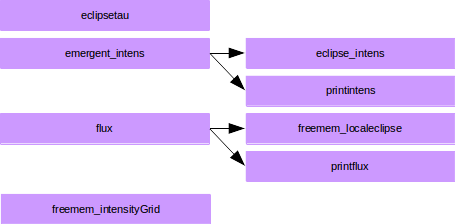
\includegraphics{fig/eclipsec}
\caption{Function structure of eclipse.c. The boxes contain function names, and arrows point from a function to the function it calls. Functions are called from left to right, then top to bottom.  Boxes are color-coded as follows:  purple functions are used for eclipse geometry, blue functions are used for transit geometry, and green functions are used in both.}
\label{fig:eclipsec}
\end{figure}

\subsubsection{List of Functions Defined in eclipse.c:}
\function{
static PREC\_RES eclipsetau(struct transit *tr, PREC\_RES height, PREC\_RES *ex)}
\tgray{Computes optical depth for eclipse geometry for one ray and one wavenumber at various incident angles on the planet surface, between a certain layer in the atmosphere up to the top layer.}\newline

\function{
static PREC\_RES eclipse\_intens(struct transit *tr, PREC\_RES *tau, PREC\_RES w, \\
long last, double toomuch, prop\_samp *rad)}
\tgray{Calculates emergent intensity for one wavenumber.}\newline

\function{
int emergent\_intens(struct transit *tr)}
\tgray{Driver function that calculates emergent intensity for the whole range of wavenumbers at various points on the planet.}\newline

\function{
int flux(struct transit *tr)}
\tgray{Calculates flux by integrating intensity over predefined angles.}\newline

\function{
void printintens(struct transit *tr)}
\tgray{Print (to file or stdout) the emergent intensities as a function of wavelength for each angle.}\newline

\function{
void printflux(struct transit *tr)}
\tgray{Print (to file or stdout) the flux as a function of wavenumber.}\newline

\function{
freemem\_localeclipse()}
\tgray{Free eclipse pointer arrays.}\newline

\function{
freemem\_intensityGrid(struct grid *intens, long *pi)}
\tgray{Free intensity grid structure arrays.}\newline

\subsubsection{eclipsetau}
\noindent
\paragraph{Walkthrough}
\begin{enumerate}[leftmargin=10pt, noitemsep, parsep=0pt, topsep=0ex]
\item[-] Use a binary search to find the index of the sampled radius immediately below or equal to the height.
\item[-] Check if the sampled radius is the outer layer, and if so return 0.
\item[-] Move pointers to the location of height.
\item[-] Check that there are sufficient points for spline integration. If not, create them halfway between the given points.
\item[-] Calculate the distance along the path for each radius.
\item[-] Allocate auxillary arrays for integration.
\item[-] Call to \ttblue{makeh} from spline.c to calculate spacing array for integration.
\item[-] Call to \ttblue{geth} from spline.c to calculate auxillary integration arrays.
\item[-] Call to \ttblue{simps} from spline.c to perform Simpson's integration of the extinction along the light path.
\item[-] Return optical depth per unit radius.
\end{enumerate}

\subsubsection{eclipse\_intens:}
\paragraph{Walkthrough}
\begin{enumerate}[leftmargin=10pt, noitemsep, parsep=0pt, topsep=0ex]
\item[-] Calculate the Planck blackbody function for each radial layer. See Equation \ref{eqn:planck}.
\item[-] Calculate the transmission function for each layer of the planet. This is the integrand of the integral in Equation \ref{eqn:intens}.
\item[-] After tau reaches toomuch, fill remaining layers with 0 flux.
\item[-] Check that there are enough points for Simpson's integration.
\item[-] Allocate auxillary arrays for integration.
\item[-] Call to \ttblue{makeh} from spline.c to calculate spacing array for integration.
\item[-] Call to \ttblue{geth} from spline.c to calculate auxillary integration arrays.
\item[-] Call to \ttblue{simps} from spline.c to perform Simpson's integration of optical depth up to the maximum optical depth to calculate intensity. See Equation \ref{eqn:intens}.
\item[-] Return integration result (intensity).
\end{enumerate}

\subsubsection{emergent\_intens:}
\paragraph{Variables Modified}
\begin{enumerate}[leftmargin=10pt, noitemsep, parsep=0pt, topsep=0ex]
\item[-] Call {\tt eclipse\_intens} to calculate \ttred{tr.ds.intens.a} (intensity[angle][wn]).
\item[-] Update \ttred{tr.pi} to account for {\tt TRPI\_MODULATION}.
\end{enumerate}

\noindent
\paragraph{Walkthrough}
\begin{enumerate}[leftmargin=10pt, noitemsep, parsep=0pt, topsep=0ex]
\item[-] Call \ttblue{eclipse\_intens} from eclipse.c as sol.spectrum to calculate the intensity at every wavenumber.
\item[-] Update the progress indicator to account for {\tt TRPI\_MODULATION}
\item[-] Call \ttblue{printintens} from eclipse.c to print the emergent intensity as a function of wavenumber to file.
\item[-] Return 0 on success.
\end{enumerate}

\subsubsection{flux:}
\paragraph{Variables Modified}
\begin{enumerate}[leftmargin=10pt, noitemsep, parsep=0pt, topsep=0ex]
\item[-] Allocate \ttred{tr.ds.out.o} (emergent flux)
\item[-] Calculate \ttred{tr.ds.out.o} (flux). See Equation \ref{eqn:flux}.
\end{enumerate}

\noindent
\paragraph{Walkthrough}
\begin{enumerate}[leftmargin=10pt, noitemsep, parsep=0pt, topsep=0ex]
\item[-] Allocate area grid and fill (local variable).
\item[-] Allocate array for emergent flux.
\item[-] Calculate flux from intensity grid and area.
\item[-] Call freemem\_localeclipse to free area grid.
\item[-] Call printflux to print the flux.
\item[-] Return 0 on success.
\end{enumerate}

\newpage
\subsection{slantpath.c:}
This file contains routines that calculate tau at a specific impact parameter and wavenumber, and routines that calculate modulation for a specific wavenumber. \ttblue{totaltau2}, which is intended to calculate tau taking into account a variable index of refraction, is unused and untested. Figure \ref{fig:slantpathc} shows the function structure of slantpath.c.

\begin{figure}
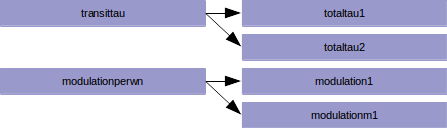
\includegraphics{fig/slantpathc}
\caption{Function structure of slantpath.c. The boxes contain function names, and arrows point from a function to the function it calls. Functions are called from left to right, then top to bottom.  Boxes are color-coded as follows:  purple functions are used for eclipse geometry, blue functions are used for transit geometry, and green functions are used in both.}
\label{fig:slantpathc}
\end{figure}

\subsubsection{List of Functions Defined in slantpath.c:}
\function{
static PREC\_RES totaltau1(&PREC\_RES b, PREC\_RES *rad, PREC\_RES refr,
                        \\ &PREC\_RES *ex, long nrad)}
\tgray{Compute the light path and optical depth at a given impact parameter
     and wavenumber, for a medium with constant index of refraction.} \newline

\function{
static PREC\_RES totaltau2(&PREC\_RES b, PREC\_RES *rad, PREC\_RES *refr,
                        \\ &PREC\_RES *ex, long nrad)}
\tgray{Compute the light path and optical depth at a given impact parameter
     and wavenumber, for a medium with variable index of refraction.} \newline

\function{
static inline PREC\_RES transittau(&PREC\_RES b, PREC\_RES *rad, PREC\_RES *refr,
                              \\ &PREC\_RES *ex, long nrad, int exprlevel)}
\tgray{Driver function to calculate the optical depth at a given impact
       parameter at a specific wavenumber.} \newline

\function{
static PREC\_RES modulationperwn(&PREC\_RES *tau, long last, double toomuch,
                              \\ &prop\_samp *ip, struct geometry *sg,
                              \\ &int exprlevel)}
\tgray{Driver function to calculate the modulation in/out-of-transit ratio for a single wavenumber.} \newline

\function{
static PREC\_RES modulation1(&PREC\_RES *tau, long last, double toomuch,
                          \\ &prop\_samp *ip, struct geometry *sg)}
\tgray{Calculate the transit's modulation at a given wavenumber for
no-limb darkening nor emitted flux.} \newline

\function{
static inline PREC\_RES modulationm1(&PREC\_RES *tau, long last, double toomuch,
                                  \\ &prop\_samp *ip, struct geometry *sg)}
\tgray{Calculate the modulation at a given wavenumber, considering the planet
as an opaque disc of radius r = r(tau=toomuch), for no-limb darkening
nor planet emission.} \newline


\subsubsection{totaltau1:}
\paragraph{Walkthrough:}
\begin{enumerate}[leftmargin=10pt, noitemsep, parsep=0pt, topsep=0ex]
\item[-] Calculate the minimum distance of the ray path to the center
  of the planet ({\tt r0}).
\item[-] Get the index ({\tt rs}) of the sampled radius below or equal
  to {\tt r0}.
\item[-] Move the extinction and radius pointers to {\tt rs}.
\item[-] Calculate the extinction coefficient at the closest approach
  radius by parabolic interpolation.
\item[-] If there are only two elements in the extinction and radius
  arrays, create a 3rd temporary element between the two values.
\item[-] Calculate the distance along the lightray path.
\item[-] Allocate auxillary arrays for integration.
\item[-] Call to \ttblue{makeh} from spline.c to calculate spacing array for integration.
\item[-] Call to \ttblue{geth} from spline.c to calculate auxillary integration arrays.
\item[-] Call to \ttblue{simps} from spline.c to perform Simpson's integration to calculate the optical depth by integrating the
  extinction along the ray path (up to the closest approach). See Equation \ref{eqn:tau}.
\item[-] Reset the original values of the extinction and radius arrays
  (in case of 2 elements).
\item[-] Return the result of integration to account for full
 multiplied by 2.
\end{enumerate}

\subsubsection{totaltau2:}
\paragraph{Walkthrough:}
\begin{enumerate}[leftmargin=10pt, noitemsep, parsep=0pt, topsep=0ex]
\item[-] Warn user that this routine is untested (and surely will not work).
\item[-] Calculate the minimum distance of the ray path to the center
  of the planet ({\tt r0}).
\item[-] Get the index ({\tt rs}) of the sampled radius below or equal
  to {\tt r0}.
\item[-] Move the radius pointer to the element corresponding to the
  sampled radius index.
\item[-] Calculate the analytical part of the extinction integral.
\item[-] Allocate auxillary arrays for integration.
\item[-] Call to \ttblue{makeh} from spline.c to calculate spacing array for integration.
\item[-] Call to \ttblue{geth} from spline.c to calculate auxillary integration arrays.
\item[-] Call to \ttblue{simps} from spline.c to perform Simpson's integration to calculate the optical depth by integrating if
  there are at least 3 points available. See Equation \ref{eqn:tau}.
\item[-] Return the result of integration multiplied by 2 to account for full path.
\end{enumerate}


\subsubsection{transittau:}
\paragraph{Variables Modified:}
\begin{enumerate}[leftmargin=10pt, noitemsep, parsep=0pt, topsep=0ex]
\item[-] Set \ttred{tr.taulevel} from {\tt th.taulevel} (Constant or
  variable index of refraction per layer).
\end{enumerate}

\paragraph{Walkthrough:}
\begin{enumerate}[leftmargin=10pt, noitemsep, parsep=0pt, topsep=0ex]
\item[-] Read the taulevel flag to determine a constant or variable
  index of refraction.
\item[-] Call to \ttblue{totaltau1} or \ttblue{totaltau2} depending on
  taulevel.
\item[-] Return the value given by \ttblue{totaltau1} or \ttblue{totaltau2}.
\end{enumerate}


\subsubsection{modulation1:}
\paragraph{Walkthrough:}
\begin{enumerate}[leftmargin=10pt, noitemsep, parsep=0pt, topsep=0ex]
\item[-] Get the stellar radius.
\item[-] Calculate integrand of modulation. See Equation \ref{eqn:mod}.
\item[-] Add a layer with an integrand value of 0.
\item[-] Raise an error if there are not enough points for integration.
\item[-] Allocate auxillary arrays for integration.
\item[-] Call to \ttblue{makeh} from spline.c to calculate spacing array for integration.
\item[-] Call to \ttblue{geth} from spline.c to calculate auxillary integration arrays.
\item[-] Call to \ttblue{simps} from spline.c to perform Simpson's integration of the integrand along radius.
\item[-] Subtract the total area blocked by the planet.
\item[-] Adjust the result if the planet is transparent.
\item[-] Normalize to the stellar radius.
\item[-] Return the modulation.
\end{enumerate}

\subsubsection{modulationm1:}
\paragraph{Walkthrough:}
\begin{enumerate}[leftmargin=10pt, noitemsep, parsep=0pt, topsep=0ex]
\item[-] If toomuch was not reached, return -1.
\item[-] Find the impact parameter before and after tau reached toomuch.
\item[-] Use linear interpolation to calculate planet radius.
\item[-] Calculate and return the modulation assuming the planet is an opaque disc (R\sp{2}/R\sp{2}\sb{*}).
\end{enumerate}

\subsubsection{modulationperwn:}
\paragraph{Variables Modified:}
\begin{enumerate}[leftmargin=10pt, noitemsep, parsep=0pt, topsep=0ex]
\item[-] Set \ttred{tr.modlevel} from {\tt th.modlevel}.
\end{enumerate}

\paragraph{Walkthrough:}
\begin{enumerate}[leftmargin=10pt, noitemsep, parsep=0pt, topsep=0ex]
\item[-] Read the modlevel flag to calculate the modulation using the
  optical-depth per impact parameter (modulation1) or an opaque disk
  of radius r = r(tau=toomuch).
\item[-] Call to \ttblue{modulation1} or \ttblue{modulationm1} depending on
  modlevel.
\item[-] Return the value given by \ttblue{modulation1} or \ttblue{modulationm1}.
\end{enumerate}


\newpage
\subsection{observable.c:}
This file contains \ttblue{modulation}, a routine which uses \ttblue{modulationperwn} to calculate modulation at each wavenumber. Figure \ref{fig:observablec} shows the function structure of observable.c.

\begin{figure}
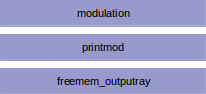
\includegraphics{fig/observablec}
\caption{Function structure of observable.c. The boxes contain function names, and arrows point from a function to the function it calls. Functions are called from left to right, then top to bottom.  Boxes are color-coded as follows:  purple functions are used for eclipse geometry, blue functions are used for transit geometry, and green functions are used in both.}
\label{fig:observablec}
\end{figure}

\subsubsection{List of Functions Defined in observable.c:}
\function{
int modulation(struct transit *tr)}
\tgray{Calculate the transit modulation at each wavenumber.} \newline

\function{
void printmod(struct transit *tr)}
\tgray{Print (to file or stdout) the modulation as function of wavelength.} \newline

\function{
int freemem\_outputray(struct outputray *out, long *pi)}
\tgray{Free the transit modulation array.} \newline

\subsubsection{modulation}
\paragraph{Variables Modified}
\begin{enumerate}[leftmargin=10pt, noitemsep, parsep=0pt, topsep=0ex]
\item[-] Allocate \ttred{tr.ds.out.o} (modulation output).
\item[-] Call to {\tt setgeom} from geometry.c to calculate \ttred{tr.ds.sg.x, tr.ds.sg.y} (coordinates of the center of the planet with respect to the star).
\item[-] Call to {\tt modulationperwn} to calculate \ttred{tr.ds.out.o} (modulation).
\end{enumerate}

\paragraph{Walkthrough}
\begin{enumerate}[leftmargin=10pt, noitemsep, parsep=0pt, topsep=0ex]
\item[-] Allocate modulation output.
\item[-] Check that tau, makeipsample, and makewnsample functions have been called.
\item[-] Call \ttblue{setgeom} to calculate X and Y values (center of the planet with respect to the star). Note that these values are not currently used by the function, and are intended to be used to account for limb-darkening.
\item[-] Call \ttblue{moldulationperwn} as sol.spectrum from slantpath.c to calculate modulation.
\item[-] Update the progress indicator to account for {\tt TRPI\_MODULATION}.
\item[-] Call printmod to print the modulation to file.
\end{enumerate}
\newpage

\comment{
\section{These Sections do not belong to the Code Doc!}

\subsection{Extinction Coefficient:}
The molecular extinction coefficient is calculated following Equations
(3.36)--(3.37) in cgs-Gaussian units as:
\begin{equation}
\label{eq:extinction}
  e_m = \frac{\pi e^2}{c^2 m_e} \sum_i \frac{\rho_i}{m_i} \frac{gf_i}{Z_i}
      \exp\left(-\frac{hcE_{\rm low}^i}{kT}\right)
      \left(1-\exp\left(\frac{hc\bar\nu_0^i}{kT}\right)\right)
      \Psi(\bar\nu, \alpha_D, \alpha_L),
\end{equation}
where $gf_i$ is the weighted oscillator strength (\texttt{ltgf =
}\ttred{tr.ds.li.lt.gf}), $Z_i$ is the partition function
(\texttt{ziso = }\ttred{tr.ds.iso.isov.z}), $\bar\nu_0^i$ is the line
wavenumber (\texttt{wavn = 1/}\ttred{tr.ds.li.lt.wl}), $E_{\rm low}^i$
the lower state energy level (\texttt{ltelow =
}\ttred{tr.ds.li.lt.elow}, in cm$^{-1}$), $T$ is the atmospheric
temperature (\texttt{temp = }\ttred{tr.atm.t}), $\rho_i$ is the
isotopic density (\texttt{densiso = }\ttred{tr.ds.iso.isov.d}), and
$m_i$ is the isotope's mass (\texttt{mass =
}\ttred{tr.ds.iso.isov.m}).  $\Psi$ is the Voigt line profile
(\texttt{profwn = profile}, in cm), where $\alpha_D$, and $\alpha_L$
are the Doppler and Lorentz line-broadening widths.  The constants in
the equation are: $e$ is the electron charge (in statC), $m_e$ the
electron mass, $k$ the Boltzmann constant, $h$ the Planck constant,
$c$ the speed of light.


The Doppler and Lorentz widths:
\begin{eqnarray}
\label{eq:doppler}
 \alpha_D &=& \underbrace{\frac{\sqrt{2k T \ln{2}}}{c}}_{\rm{propto\_adop}}
              \frac{\bar\nu_0}{\sqrt{m_i}} \label{dopbr} \\
\label{eq:lorentz}
 \alpha_L &=& \underbrace{\sqrt{\frac{2k T}{\pi^3c^2}}}_{\rm{propto\_alor}}
              \sigma_c\sum_{\rm coll}\frac{\rho_j}{m_j}
              \sqrt{\left(\frac{1}{m_j} + \frac{1}{m_i}\right)}
              + \underbrace{\alpha_{N}}_{\mathrm{ignored}}
\end{eqnarray}
where $\sigma_c$ is the cross section of the isotope (\texttt{csiso =
}\ttred{tr.ds.iso.isov.c}), $m_j$ is the mass of the colliding
isotope, $\rho_j$ is the density of the colliding isotope, and
$\alpha_N$ is the natural broadening (which is negligible compared to
the collisional broadening).

Note that, actually, $\alpha_D$ is the Doppler half-width at half
maximum (where the Doppler width is defined as HWHM/$\sqrt{\ln 2}$).
Since the Doppler profile depends on the wavenumber, the profile must
be recalculated every certain range in wavenumber. \newline

\subsection{HITRAN Line Strength to $gf$ Conversion:}

The HITRAN database \citep{Rothman2013JqsrtHITRAN} provides the line
intensity (cm$^{-1}$/(molecule cm$^{-2}$)), which needs to be
converted to the dimensionless $gf$ value.  Equation (20) of
\citet{Simeckova2006JqsrtHITRAN} gives the line intensity ($S$) in
terms of the Einstein $A_{21}$ coefficient:

\begin{equation}
S = A_{21} \frac{I_a g_2}{8\pi c \nu_0^2}
           \frac{1}{Z(T_0)}
           \exp\left(\frac{-hcE_1}{kT_0}\right)
           \left(1-\exp\left(\frac{-hc\nu_0}{kT_0}\right)\right),
\end{equation}
where $I_a$ is the isotopic abundance, $g_i$ the statistical weight of
the level $i$, $c$ the speed of light, $\nu_0$ is the line wavenumber,
$Z$ is the partition function, $T_0$ is the HITRAN standard
temperature, $h$ the Planc constant, $E_1$ the lower state energy
level (in cm$^{-1}$), and $k$ the Boltzmann constant.

Replacing the Einstein $A_{21}$ coefficient by the
oscillator strength ($f_{12}$) from her Equation (36), where
$epsilon_0$ is replaced by $1/(4\pi)$ when working in cgs units:
\begin{equation}
A_{21} = \frac{g_1}{g_2}\frac{8 \pi^2 e^2 \nu_0^2}{m_e c} f_{12},
\end{equation}
where $e$ is the electron charge (in statCoulomb), $m_e$ the
electron charge, and $f_{12}$ the oscillator strength.
Then, we have for the line intensity:
\begin{equation}
S = I_a \frac{g_1 f_{12}}{Z(T_0)} \frac{\pi e^2} {m_e c^2}
        \exp\left(\frac{-hcE_1}{kT_0}\right)
        \left(1-\exp\left(\frac{-hc\nu_0}{kT_0}\right)\right),
\end{equation}
and finally:
\begin{equation}
gf = g_1 f_{12} = S \frac{m_e c^2} {\pi e^2} \frac{Z(T_0)}{I_a} 
        \exp\left(\frac{hcE_1}{kT_0}\right)
        \left(1-\exp\left(\frac{-hc\nu_0}{kT_0}\right)\right)^{-1}.
\end{equation}

\subsection{Density Calculation:}

The abundances in the atmosphere file can be given either as a mass
fraction ($\mu$, mass mixing ratio) or as a number fraction ($\nu$,
mixing ratio):
\begin{equation}
\mu_i = \frac{m_in_i}{m}; \qquad \nu_i = \frac{n_i}{n},
\end{equation}
with $n_i$ and $m_i$ the mass and number of molecules of species $i$,
$m$ and $n$ the total mass and number of molecules in the layer.

The density profiles are calculated using the ideal gas law in the form:
\begin{equation}
p = \frac{n}{V}kT,
\label{eq:igaslaw}
\end{equation}
with $p$, $T$, $V$ the total pressure, temperature, and volume of the
layer.  Recognizing that the partial density can be written as:
\begin{equation}
\rho_i = \frac{m_in_i}{V},
\end{equation}
and replacing the volume from Equation (\ref{eq:igaslaw}), we have:
\begin{equation}
  \rho_i = \frac{m_in_i}{n}\frac{P}{kT},
\end{equation}
wich can be restated as:
\begin{equation}
  \rho_i = m_i\frac{n_i}{n}\frac{P}{kT} = m_i\nu_i\frac{P}{kT},
\end{equation}
or as:
\begin{equation}
  \rho_i = \frac{\mu_im}{n}\frac{P}{kT} = \bar{m}\mu_i\frac{P}{kT},
\end{equation}
with $\bar{m} = m/n$, the mean molecular mass in the layer.


\subsection{Radiative Transfer:}

\subsubsection{Some definitions to begin:}
The specific intensity ($I\sb{\nu}$) is the
energy (d$E$) between frequencies $\nu$ and $\nu$ + d$\nu$ per unit
time (d$t$) that flows through a unit surface area (d$A$) at an angle
$\theta$ (measured with respect to the normal) contained in a solid
angle (d$\Omega$):

\begin{equation}
I\sb{\nu} = \frac{\der E}{\cos\theta \der A \der\Omega \der\nu \der t},
\end{equation}
with units of ergs s\tno cm\tnt sr\tno Hz\tno.  The specific flux
($F\sb{\nu}$) is the net energy between frequencies $\nu$ and $\nu$ +
d$\nu$ per unit time that flows perpendicularly through a unit surface
area, i.e., the specific intensity integrated over solid angle:

\begin{equation}
F\sb{\nu} = \int I\sb{\nu} cos\theta \der\Omega
\end{equation}
with units of ergs s\tno cm\tnt Hz\tno.

\subsubsection{On to the radiative transfer equation:} 
When a ray of light passes
through a medium its intensity decreases due to the absorption or
scattering from particles. This is proportional to the intensity
itself, to the medium density ($\rho$), to the absorption coefficient
(or opacity, $\kappa\sb{\nu}$) and the path traveled ($\der s$):

\begin{equation}
\der I\sb{\nu} = - I\sb{\nu} \kappa\sb{\nu} \rho \der s.
\end{equation}
The opacity is the cross section of photons at frequency $\nu$ per
unit mass.  Additionally, the medium can also contribute to the
intensity, this is described by the emission coefficient
($j\sb{\nu}$), the rate of change in intensity by the emission
coefficient is proportional to the density and the path traveled:

\begin{equation}
\der I\sb{\nu} =  j\sb{\nu} \rho \der s.
\end{equation}
Let's define the source function $S\sb{\nu} =
j\sb{\nu}/\kappa\sb{\nu}$ and the optical depth ($\chi$) as $\der
\chi = \kappa\sb{\nu} \rho \der s$, the transfer equation becomes:
\begin{equation}
\frac{\der I\sb{\nu}}{\der \chi} = - I\sb{\nu}  +  S\sb{\nu}.
\end{equation}

\subsubsection{Emergent Flux:} 

To study the case of the flux emitted by a planet (or star), first
assume the plane-parallel approximation, which is valid when the
vertical scale is much smaller than the horizontal scale.  In this
case we can safely assume that the atmosphere is composed by a
stratified set of plane slabs with uniform properties.

Defining $\tau = -\kappa\sb{\nu} \rho \der z$ as the vertical optical
depth (note the negative sign in the definition, that implies that
$\tau=0$ at the top of the atmosphere, increasing inward).  The path
for a ray ($\der s$) with an angle $\theta$ with respect to the
vertical is related to the vertical path as: $\der s = \der
z/\cos\theta \equiv \der z / \mu$, and thus the RT equation becomes:
\begin{equation}
-\mu\frac{\der I\sb{\nu}}{\der \tau} = - I\sb{\nu}  +  S\sb{\nu}.
\end{equation}
To sove, multiply by $\exp(-\tau/\mu)$:
\begin{eqnarray}
-\mu\frac{\der I\sb{\nu}}{\der \tau}e\sp{-\tau/\mu} + I\sb{\nu}e\sp{-\tau/\mu}  & = & S\sb{\nu}e\sp{-\tau/\mu} \\
-\mu\frac{\der}{\der \tau}\left( I\sb{\nu}e\sp{-\tau/\mu} \right)  & = & S\sb{\nu}e\sp{-\tau/\mu}
\end{eqnarray}

For the emerging intensity at the top of the atmosphere ($\tau=0$),
consider a depth where the atmosphere is well optically thick,
$\tau=\tau\sb{b}$, such $exp{-\tau\sb{b}/\mu} \to 0$, then:
\begin{eqnarray}
\Eval{-I\sb{\nu}e\sp{-\tau/\mu}}{0}{\tau\sb{b}}  & = &
     \int\sb{0}\sp{\tau\sb{b}}S\sb{\nu}e\sp{-\tau/\mu}\der\tau/\mu \\
I(0)  & = &
     \int\sb{0}\sp{\tau\sb{b}}S\sb{\nu}e\sp{-\tau/\mu}\der\tau/\mu
\label{eq:topatmint}
\end{eqnarray}

Under LTE, the source function becomes the Planck function $B\sb{\nu}(T)$.
To obtain the emergent flux, integrate the solid angle over the half sphere:
\begin{equation}
F\sb{\nu} =      \int\sb{0}\sp{2\pi}\int\sb{0}\sp{\pi/2} I\sb{\nu} \cos\theta\sin\theta \der\theta \der\phi 
          = 2\pi \int\sb{0}\sp{\pi/2} I\sb{\nu} \cos\theta\sin\theta \der\theta
          = 2\pi \int\sb{0}\sp{1}     I\sb{\nu} \mu\der\mu.
\end{equation}

Combined with Equation \ref{eq:topatmint}:
\begin{equation}
F\sb{\nu}(0) = 2\pi \int\sb{0}\sp{1} \int\sb{0}\sp{\tau\sb{b}} B\sb{\nu}e\sp{-\tau/\mu}\der(\tau/\mu)\, \mu\der\mu
\end{equation}

To solve this equation, use the diffuse approximation where we
replace $\tau/\mu \approx \tau/\bar{\mu}$, with $1/\bar{\mu} = 5/3 =
1.66$, the diffusivity factor.  Then:
\begin{eqnarray}
F\sb{\nu}(0) & = & 2\pi \int\sb{0}\sp{\tau\sb{b}} B\sb{\nu}e\sp{-\tau/\bar{\mu}}\der(\tau/\bar{\mu})\, \int\sb{0}\sp{1}\mu\der\mu \\
             & = & 2\pi \int\sb{0}\sp{\tau\sb{b}} B\sb{\nu}e\sp{-\tau/\bar{\mu}}\der(\tau/\bar{\mu})\, \frac{1}{2}
\end{eqnarray}

Finally the emerging flux at the top of the atmosphere is:
\begin{equation}
F\sb{\nu}(0) = \pi \int\sb{0}\sp{\tau\sb{b}} B\sb{\nu}e\sp{-\tau/\bar{\mu}}\der(\tau/\bar{\mu})
\end{equation}
}
\section{Equations}
\label{sec:equations}
Optical depth:

\begin{equation}
\label{eqn:tau}
\tau = \int e \cdot \mathrm{d}s
\end{equation}
\noindent
where $e$ is extinction and d$s$ is the differential path element. \newline

\noindent
Extinction:

\begin{equation}
\label{eq:ext}
  e_m = \frac{\pi e^2}{c^2 m_e} \sum_i \frac{\rho_i}{m_i} \frac{gf_i}{Z_i}
      \exp\left(-\frac{hcE_{\rm low}^i}{kT}\right)
      \left(1-\exp\left(\frac{hc\bar\nu_0^i}{kT}\right)\right)
      \Psi(\bar\nu, \alpha_D, \alpha_L),
\end{equation}
\noindent
where $e_m$ is extinction, $gf$ is the weighted oscillator strength, $Z_i$ is the partition function, $\bar\nu_0^i$ is the central wavenumber of the line, $E_{\rm low}^i$ is the lower state energy level, $T$ is the atmospheric temperature, $\rho_i$ is the isotopic density, $m_i$ is the isotopic mass, $\Psi$ is the Voigt line profile (the convolution of Doppler and Lorentz profiles) with arguments of central wavenumber ($\bar\nu$), Doppler width ($\alpha_D$), and Lorentz width ($\alpha_L$). $k$ is the Boltzmann constant, $h$ is the Planck constant, and $c$ is the speed of light.  \newline

\noindent
Doppler and Lorentz widths:

\begin{eqnarray}
\label{eqn:doppler}
 \alpha_D &=& \underbrace{\frac{\sqrt{2k T \ln{2}}}{c}}_{\rm{propto\_adop}}
              \frac{\bar\nu_0}{\sqrt{m_i}} \label{dopbr} \\
\label{eqn:lorentz}
 \alpha_L &=& \underbrace{\sqrt{\frac{2k T}{\pi^3c^2}}}_{\rm{propto\_alor}}
              \sigma_c\sum_{\rm coll}\frac{\rho_j}{m_j}
              \sqrt{\left(\frac{1}{m_j} + \frac{1}{m_i}\right)}
              + \underbrace{\alpha_{N}}_{\mathrm{ignored}}
\end{eqnarray}
\noindent
where $\alpha_D$ is Doppler width, $\alpha_L$ is Lorentz width, $k$ is the Boltzmann constant, $T$ is atmospheric temperature, $c$ is the speed of light, $\bar\nu_0$ is central wavenumber, $m_i$ is isotopic mass, $\sigma_c$ is isotopic cross section, $\rho_j$ is isotopic density, and $\alpha_N$ is natural broadening (negligible). \newline

\noindent
Density:
\begin{equation}
\label{eqn:den}
  \rho_i = \frac{\mu_im}{n}\frac{P}{kT} = \bar{m}\mu_i\frac{P}{kT},
\end{equation}
\noindent
where $\mu_i$ is the mass mixing ratio, $m$ is mass, $P$ is pressure, $k$ is the Boltzmann constant, $T$ is temperature, and where $\bar{m} = m/n$, the mean molecular mass in the layer.\newline

\noindent
Modulation:
\begin{equation}
\label{eqn:mod}
M_{\lambda} = \frac{1}{R_\star^2}\left(R^2 - 2\int_{0}^{R} \exp^{-\tau_\lambda(r)} r\,{\rm d}r\right)
\end{equation}

\noindent
where $R_{*}$ is the stellar radius, $\tau_\lambda$ is optical depth at a particular wavelength as a function of radius, and $R$ is the planetary radius. \newline

\noindent
Planck function for wavenumbers:
\begin{equation}
\label{eqn:planck}
B_\nu = 2 h {\bar\nu}^3 c^2 \frac{1}{\exp(\frac{h \bar \nu c}{k_B T})-1}
\end{equation}

\noindent
where $\nu$ is wavenumber, $h$ is the Planck constant, $c$ is the speed of light, $k_B$ is the Boltzmann constant, and $T$ is temperature. \newline

\noindent
Emergent intensity:
\begin{equation}
\label{eqn:intens}
I = \int_0\sp{\tau\sb{max}} B_\nu \mathrm{e}^{-\tau} \mathrm{d}\tau
\end{equation}

\noindent
where $B_\nu$ is the Planck blackbody function and $\tau$ is optical depth. The integral is from $0$ to {\tt tr.toomuch}. \newline

\noindent
Flux:
\begin{equation}
\label{eqn:flux}
F = \sum\limits_{i=1} \pi I_i ((\sin{\theta_{fin}})^2 - (\sin{\theta_{in}})^2)
\end{equation}

\noindent
where $I$ is intensity, $A$ is area, $n$ is the number of angles, and $w_n$ is the number of wavenumbers. \newline

\noindent
Hydrostatic pressure:
\begin{equation}
\label{eqn:hydrostatic}
\frac{dP}{P} = -\frac{dz}{H}
\end{equation}

\noindent
where $P$ is pressure, $z$ is height, and $H$ is scale height. \newline
\bibliography{transit}
\end{document}


